% !TEX program = xelatex
% !TEX option = -shell-escape
% Generated by tools/build_latex.py; edit chapter fragments, not Markdown.
\documentclass[bwprint]{gmcmthesis}
\geometry{top=25mm,bottom=25mm,left=25mm,right=25mm,headsep=15mm}
\renewcommand{\baselinestretch}{1.0}
\normalsize
\def\GMCMEvaluationSection{7}
\hypersetup{hidelinks}
\renewcommand{\thesubsection}{\arabic{section}.\arabic{subsection}}
\renewcommand{\thesubsubsection}{\thesubsection.\arabic{subsubsection}}
\pagestyle{plain}
\usepackage[framemethod=TikZ]{mdframed}
\usepackage{subfig}
\usepackage{siunitx}
\usepackage{colortbl}
\usepackage{array}
\usepackage{tabularx}
\usepackage{longtable}
% AI usage is recorded in the actual bibliography; no template assertion.
% 华为杯统一附录模板。
% 本文件由 build_latex.py 复制到论文目录并在导言区实际 \input；
% 生成内容只能调用这里的接口，不得在章节片段中另设代码样式。
\usepackage{minted}
\usepackage{xcolor}
\usepackage{tcolorbox}
\tcbuselibrary{breakable,skins}
\usepackage{longtable}
\usepackage{booktabs}
\usepackage{array}
\usepackage{needspace}
\usemintedstyle{lovelace}

% 克制的浅色学术代码配色。语法 token 由 Pygments 的 lovelace 浅色主题生成；
% 下列颜色只负责纸面、边线和行号，不覆盖 Pygments token 语义。
\definecolor{AppendixStripeWhite}{HTML}{FFFFFF}
\definecolor{AppendixStripeGray}{HTML}{F8F8F8}
\definecolor{AppendixDivider}{HTML}{63B96C}
\definecolor{AppendixHorizontalRule}{HTML}{555B57}
\definecolor{AppendixLineNumber}{HTML}{6F8175}
\definecolor{AppendixCaption}{HTML}{343A36}
\newfontfamily\AppendixCodeLatin{Consolas}[Scale=MatchLowercase]
\newcommand{\AppendixCodeFont}{\songti\AppendixCodeLatin}
\renewcommand{\myFont}{\AppendixCodeFont}

% Pygments 仍负责词法分类；在 lovelace 浅色基底上将论文要求的
% “关键词紫、字符串绿、数字/类型棕橙、注释灰绿”固化为低饱和调色板。
% Minted 在首次代码块前载入 Pygments style，因此在 MintedVerbatim
% 开始时覆写 token 显示色，避免被后载入的 styledef 反向覆盖。
\makeatletter
\newcommand{\AppendixPygmentsPalette}{%
  \@namedef{PYG@tok@k}{\def\PYG@tc####1{\textcolor[HTML]{8B4E8F}{####1}}}%
  \@namedef{PYG@tok@kc}{\def\PYG@tc####1{\textcolor[HTML]{8B4E8F}{####1}}}%
  \@namedef{PYG@tok@kd}{\def\PYG@tc####1{\textcolor[HTML]{8B4E8F}{####1}}}%
  \@namedef{PYG@tok@kn}{\def\PYG@tc####1{\textcolor[HTML]{8B4E8F}{####1}}}%
  \@namedef{PYG@tok@kp}{\def\PYG@tc####1{\textcolor[HTML]{8B4E8F}{####1}}}%
  \@namedef{PYG@tok@kr}{\def\PYG@tc####1{\textcolor[HTML]{8B4E8F}{####1}}}%
  \@namedef{PYG@tok@kt}{\def\PYG@tc####1{\textcolor[HTML]{8B4E8F}{####1}}}%
  \@namedef{PYG@tok@ow}{\def\PYG@tc####1{\textcolor[HTML]{8B4E8F}{####1}}}%
  \@namedef{PYG@tok@s}{\def\PYG@tc####1{\textcolor[HTML]{4F8A55}{####1}}}%
  \@namedef{PYG@tok@s1}{\def\PYG@tc####1{\textcolor[HTML]{4F8A55}{####1}}}%
  \@namedef{PYG@tok@s2}{\def\PYG@tc####1{\textcolor[HTML]{4F8A55}{####1}}}%
  \@namedef{PYG@tok@sa}{\def\PYG@tc####1{\textcolor[HTML]{4F8A55}{####1}}}%
  \@namedef{PYG@tok@sd}{\def\PYG@tc####1{\textcolor[HTML]{4F8A55}{####1}}}%
  \@namedef{PYG@tok@si}{\def\PYG@tc####1{\textcolor[HTML]{4F8A55}{####1}}}%
  \@namedef{PYG@tok@m}{\def\PYG@tc####1{\textcolor[HTML]{A06D20}{####1}}}%
  \@namedef{PYG@tok@mi}{\def\PYG@tc####1{\textcolor[HTML]{A06D20}{####1}}}%
  \@namedef{PYG@tok@mf}{\def\PYG@tc####1{\textcolor[HTML]{A06D20}{####1}}}%
  \@namedef{PYG@tok@mh}{\def\PYG@tc####1{\textcolor[HTML]{A06D20}{####1}}}%
  \@namedef{PYG@tok@mo}{\def\PYG@tc####1{\textcolor[HTML]{A06D20}{####1}}}%
  \@namedef{PYG@tok@nb}{\def\PYG@tc####1{\textcolor[HTML]{9A702D}{####1}}}%
  \@namedef{PYG@tok@c}{\def\PYG@tc####1{\textcolor[HTML]{7A887E}{####1}}}%
  \@namedef{PYG@tok@c1}{\def\PYG@tc####1{\textcolor[HTML]{7A887E}{####1}}}%
  \@namedef{PYG@tok@cm}{\def\PYG@tc####1{\textcolor[HTML]{7A887E}{####1}}}%
  \@namedef{PYG@tok@cp}{\def\PYG@tc####1{\textcolor[HTML]{6F8175}{####1}}}%
}
% 用 fvextra 的全宽行盒绘制白/极浅灰逻辑行底纹。breaklines 产生的
% 视觉续行仍位于同一个 parbox 中，因此保持与源代码逻辑行相同的底色。
\newcommand{\AppendixFullWidthStripe}[2]{%
  \setlength{\FV@TmpLength}{\fboxsep}%
  \setlength{\fboxsep}{0pt}%
  \colorbox{#1}{%
    \setlength{\fboxsep}{\FV@TmpLength}%
    \rlap{\strut#2}%
    \hspace{\linewidth}%
    \ifx\FV@RightListFrame\relax\else
      \hspace{-\FV@FrameSep}\hspace{-\FV@FrameRule}%
    \fi
    \ifx\FV@LeftListFrame\relax\else
      \hspace{-\FV@FrameSep}\hspace{-\FV@FrameRule}%
    \fi
  }%
  \hss
}
\newcommand{\AppendixZebraLine}[1]{%
  \ifodd\value{FancyVerbLine}%
    \AppendixFullWidthStripe{AppendixStripeWhite}{#1}%
  \else
    \AppendixFullWidthStripe{AppendixStripeGray}{#1}%
  \fi
}
\AtBeginEnvironment{MintedVerbatim}{\AppendixPygmentsPalette}
\makeatother

% 透明、无左右框的可分页外壳。overlay 会在 unbroken/first/middle/last
% 每个物理分片上执行，从而显式重复绘制上下细横线。
\newtcolorbox{AppendixCodePageFrame}{%
  enhanced jigsaw,
  breakable,
  width=\linewidth,
  colback=white,
  colframe=AppendixHorizontalRule,
  boxrule=0pt,
  leftrule=0pt,
  rightrule=0pt,
  toprule=0pt,
  bottomrule=0pt,
  boxsep=0pt,
  left=0pt,
  right=0pt,
  % 为每个物理分页片段的横线保留极窄的无遮挡带，避免首/末行
  % 的全宽 zebra 色块覆盖横线主体。
  top=1.5pt,
  bottom=1.5pt,
  arc=0pt,
  outer arc=0pt,
  sharp corners,
  before skip=0.15\baselineskip,
  after skip=0.20\baselineskip,
  lines before break=3,
  overlay={%
    \draw[AppendixHorizontalRule,line width=0.5pt]
      ([yshift=-0.25pt]frame.north west)--([yshift=-0.25pt]frame.north east);%
    \draw[AppendixHorizontalRule,line width=0.5pt]
      ([yshift=0.25pt]frame.south west)--([yshift=0.25pt]frame.south east);%
  }
}

\setminted{
  encoding=utf8,
  linenos,
  numberblanklines=true,
  numbersep=6pt,
  breaklines,
  breakanywhere,
  autogobble,
  tabsize=4,
  obeytabs=true,
  fontfamily=myFont,
  fontsize=\fontsize{10.2pt}{13.5pt}\selectfont,
  baselinestretch=1.0,
  frame=leftline,
  framesep=5pt,
  framerule=0.55pt,
  rulecolor=\color{AppendixDivider},
  xleftmargin=3.15em,
  xrightmargin=0pt,
  listparameters={\setlength{\topsep}{0pt}\setlength{\partopsep}{0pt}\setlength{\parsep}{0pt}},
  resetmargins=true,
  style=lovelace
}

\newcommand{\AppendixStart}{%
  \section{附录}%
}

\newcounter{paperappendixpart}
\newcommand{\AppendixPart}[2]{%
  \par\vspace{1.3\baselineskip}%
  \phantomsection
  \setcounter{paperappendixpart}{#1}\addtocounter{paperappendixpart}{-1}\refstepcounter{paperappendixpart}%
  \noindent{\songti\fontsize{12pt}{18pt}\selectfont\bfseries 附录 #1：#2}\par
  \addcontentsline{toc}{subsection}{附录 #1：#2}%
  \vspace{0.55\baselineskip}%
}

\newcommand{\AppendixAttachmentTableBegin}{%
  \begingroup
  \renewcommand{\arraystretch}{1.18}%
  \setlength{\tabcolsep}{4pt}%
  \small
  \begin{longtable}{>{\centering\arraybackslash}p{1.0cm}p{3.0cm}p{10.0cm}}
  \toprule
  序号 & 文件夹名称 & 主要内容 \\
  \midrule
  \endfirsthead
  \toprule
  序号 & 文件夹名称 & 主要内容 \\
  \midrule
  \endhead
  \midrule
  \multicolumn{3}{r}{续下页}\\
  \endfoot
  \bottomrule
  \endlastfoot
}

\newcommand{\AppendixAttachmentRow}[3]{%
  #1 & #2 & #3 \\
}

\newcommand{\AppendixAttachmentTableEnd}{%
  \end{longtable}
  \endgroup
}

% #1: 可选 minted 参数（支持 firstline/lastline/firstnumber）
% #2: 代码片段标题；#3: Pygments lexer；#4: 真实源码路径。
\newcommand{\AppendixCodeFile}[4][]{%
  \Needspace{6\baselineskip}%
  \par\vspace{0.35\baselineskip}%
  \noindent{\color{AppendixCaption}\songti\fontsize{10.5pt}{15pt}\selectfont #2}\par
  \vspace{0.15\baselineskip}%
  \begingroup
  \renewcommand{\theFancyVerbLine}{\AppendixCodeLatin\fontsize{8.6pt}{13.5pt}\selectfont\color{AppendixLineNumber}\arabic{FancyVerbLine}}%
  \let\FancyVerbHighlightLine\AppendixZebraLine
  \begin{AppendixCodePageFrame}%
    \inputminted[#1]{#3}{#4}%
  \end{AppendixCodePageFrame}%
  \endgroup
  \par\vspace{0.25\baselineskip}%
}

\newcommand{\AppendixEnd}{\par}

\usepackage{paper-review}
\newcommand{\codeid}[1]{\nolinkurl{#1}}
\usepackage{booktabs}
\usepackage{tikz}
\usepackage{pgfplots}
\pgfplotsset{compat=1.18}
\usetikzlibrary{arrows.meta,positioning,fit,calc,shapes.geometric,shapes.arrows}
\makeatletter
\newcommand{\HuaweiLabel}[1]{{\lishu\fontsize{18pt}{24pt}\selectfont #1}}
\newcommand{\HuaweiBodyFont}{\songti\fontsize{12pt}{18pt}\selectfont}
\newcommand{\HuaweiTitleUnderline}[1]{%
  \begingroup
  \renewcommand{\ULthickness}{1.2pt}%
  \setlength{\ULdepth}{4pt}%
  \uline{#1}%
  \endgroup
}
\newcommand{\HuaweiPaperTitle}[1]{%
  \begin{minipage}[t]{.9\textwidth}\centering
    \HuaweiLabel{题\quad 目：}\hspace{0.4em}{\zihao{3}\heiti #1}%
  \end{minipage}%
}
\newcommand{\HuaweiTitlePage}{%
  \clearpage\thispagestyle{plain}\setcounter{page}{1}%
  \GMCMContestTitle{二十三}
  \vspace{8mm}\noindent
  \begin{center}
    \HuaweiPaperTitle{\HuaweiTitleUnderline{面向多核计算图的联合调度}\par\HuaweiTitleUnderline{与分层存储优化}}
  \end{center}
  \vspace{3mm}
}
\renewenvironment{abstract}{%
  \begin{center}\GMCMAbstractHeading\end{center}\HuaweiBodyFont\quotation
}{%
  \endquotation\clearpage
}
\renewcommand{\keywords}[1]{\par\vspace{1ex}{\noindent\HuaweiLabel{关键词：}}~{\HuaweiBodyFont #1}\par}
\makeatother
\title{面向多核计算图的联合调度与分层存储优化}

\usepackage{xurl}
\setlength{\emergencystretch}{2em}
\begin{document}
\HuaweiTitlePage
\begin{abstract}
任务组织、数据搬运和片上容量共同影响多核计算图的并行效率。本文将子图划分、核心归属与核内顺序作为联合决策，以\textbf{总体任务执行时间（Makespan）最小}为主目标，在周期相同时选择额外搬运量较小的方案。固定核内调度与全局事件推进用于计算依赖、流水线占用、自动换出和共享带宽下的执行周期，互补邻域则围绕当前可行方案搜索改进。由计算路径、流水线负载和必要搬运得到全局下界，并在题给100个计算图上考察子图任务、核心任务与共享只读缓存三种执行规则。

\textbf{针对问题一}，每个子图独立构成任务，跨子图数据经核外主存交接。为协调并行空间与边界代价，采用\textbf{多邻域迭代改进}，从依赖关键性、结构与负载生成初始方案，交替提出迁移、交换、拆分和驻留相关候选。结构条件与候选下界减少完整评价次数，字典序接受保持已取得方案可行、目标单调改善。五核\textbf{平均加速比为3.9180}，中位数为4.4227，88个五核结果未产生自动换出。每30秒记录一次已取得的可用解，用于观察有限预算内的搜索进展及逐图差异。

\textbf{针对问题二}，同一核心的全部子图构成一个任务，同核张量可延续驻留；跨核读入在相应写出完成后等待500周期再释放。采用\textbf{面向驻留与交接的候选改进}，结合张量消费者分布提出关联子图迁移和归属保持的重新分组，权衡驻留机会、容量压力与跨核并行。五核\textbf{平均加速比达到4.4538}，在两问分别寻优得到的五核方案中，100图有89图的周期短于第一问。五核额外搬运均值由第一问的14585335.66字节降至8094619.10字节；逐图搬运量有增有减，其变化与执行周期并非逐例同步。

\textbf{针对问题三}，在核心任务上加入共享只读二级缓存，按发射查询、完成填充和先进先出规则描述驻留窗口。在基础、结构与驻留候选之外加入\textbf{缓存时序候选}。纯顺序候选保持划分与归核不变，按实际填充与淘汰窗口调整子图位置；结合多尺度划分、通信感知归核和归属保持的拆分重排，通过完整评价选择方案。主实验五核\textbf{平均加速比达到4.6333}；对100图、五种核数的500组同方案缓存对照，五核平均无缓存／有缓存周期比为\textbf{1.0560}，76图周期缩短、24图相同。六图54组固定方案参数评价显示，部分方案的周期随缓存带宽增加呈非单调变化；逐事件轨迹进一步揭示了读入发射、填充与淘汰之间的时间关系。缓存分析因而同时考察有效驻留窗口与两个带宽池的竞争。

\keywords{计算图调度\quad 联合决策\quad 多邻域迭代\quad 分层存储\quad 先进先出缓存}
\end{abstract}
\setcounter{tocdepth}{3}
\clearpage
\maketoc
\clearpage
\HuaweiBodyFont
\section{问题提出}
\subsection{问题背景}

神经网络的计算可表示为带有数据依赖的有向无环图（Directed Acyclic Graph，DAG）。图中的算子完成矩阵运算、向量运算或数据搬运，张量连接前后算子并保存中间结果。执行模型推理或训练，既要安排算子的执行顺序，也要组织输入、中间结果和输出的存储与搬运。多核神经网络处理器（Neural Processing Unit，NPU）为此提供并行计算资源：各核具有矩阵、向量和搬运流水线，以及私有的一级缓存（L1）和统一缓冲区（Unified Buffer，UB）；各核访问共享核外主存（DDR）时，共同竞争固定总带宽。

增加核心数可以使互不依赖的计算同时执行，但每个算子仍需等待其输入数据就绪。若依赖链较长，部分核心会等待前驱计算；若多个核心同时读写DDR，单个请求能够获得的带宽又会下降。因此，计算工作量分配均匀并不意味着各核能同时完成任务。子图的执行次序和数据到达时刻，决定了计算流水线能否持续获得可执行的操作。

子图划分把算子组织为可调度单元。把依赖紧密的算子划入同一子图，有利于减少边界搬运和保留数据复用；但过大的子图也可能压缩跨核并行机会，并增加片上容量压力。细分子图提供更多可调度单元，却可能使同一张量被重复读取。已有DAG分组与调度研究讨论了通信与并行性的共同权衡~\cite{A49}；算子级调度研究也展示了分组方式对并行执行机会的影响~\cite{A08}。划分粒度的选择需要同时考察可释放的并行计算与新增的数据传输。

核心映射决定每个子图由哪个核心执行，核内顺序决定同核子图的先后关系。这两项决策还影响张量在片上存储中的存活区间：使用同一张量的算子相邻执行时，可在数据释放之前完成多次使用；无关操作插入其中时，则可能延长驻留并与其他张量竞争容量。容量不足引发的换出与取回又会增加DDR请求，从而把存储安排与执行时序联系起来。共享只读L2进一步提供核间的数据复用机会，其收益取决于后续算子读取时数据是否已经填充、是否仍然驻留，以及当时的读服务负载。

上述因素共同影响总体任务执行时间（Makespan），即从开始执行到全部任务完成的时间。在给定计算图、硬件参数和固定执行规则下，联合确定子图划分、核心映射与核内顺序，并在执行任务组织和存储层级不同的场景中比较结果。研究重点是解释三项决策如何改变计算等待、边界搬运和数据复用，从而形成能够缩短总体任务执行时间的完整方案。

\subsection{问题重述}

给定计算图、硬件配置及固定执行规则，需要为每个非\texttt{COPY\_IN}\slash\allowbreak\texttt{COPY\_OUT}算子指定子图编号，给出各子图的所属核心和每个核心上的子图顺序。子图须完整覆盖待分配算子，由跨子图依赖形成的子图依赖图必须无环，且每个子图在核内顺序中恰好出现一次。评估程序按照场景重建边界搬运、确定核内固定操作顺序和容量不足时的换入换出，再模拟多核心、流水线与共享带宽上的执行；其输出的总体任务执行时间是主要指标，总额外数据搬运量是次要指标。算法须在全部100个测试用例及固定参数下产生可执行方案，并提供可复现的Python脚本。

问题一对应无核间同步机制的场景A。每个子图独立构成一个执行任务（Task，即向单个核心一次下发的调度单元），所有跨子图依赖均通过DDR交接；同核任务切换等待100周期，跨核前驱任务完成后等待1000周期。需要在2～5核配置下建立子图划分与调度模型并生成方案，尽可能缩短总体任务执行时间，同时控制总额外数据搬运量。正文应按原始整图单核基准，给出1～5核的平均加速比折线图；附录须逐用例列出评估得到的总体任务执行时间与总额外数据搬运量，并提供规定格式的程序附件。

问题二对应具有核间同步机制的场景B。同一核心上的全部子图合为一个执行任务，满足容量与依赖条件时，前一子图的数据可在L1或UB中供后一子图使用；跨核依赖仍经\texttt{COPY\_OUT}/\texttt{COPY\_IN}及500周期同步延迟完成。需要在严格满足L1、UB容量约束下，沿用子图划分、核心映射与核内顺序三个决策，为2～5核配置进一步缩短总体任务执行时间并减少额外搬运。正文同样给出1～5核的平均加速比折线图，附录逐用例报告评估周期与总额外数据搬运量，附件给出可复现程序。

问题三在场景B之上加入所有核心共享的只读二级缓存（L2），按先进先出（First-In, First-Out，FIFO）规则管理，容量为1048576~B、带宽为250~B/周期，读服务带宽与DDR独立。需要研究L2容量和带宽对子图划分与调度的影响，建立相应模型并在核数变化时生成合法方案。正文应给出1～5核下无L2与有只读L2两种配置的对比曲线，并以同核数无L2的总体任务执行时间除以有L2的周期，报告只读缓存相对无L2配置的加速比；附录须逐用例列出两种配置的周期、总额外数据搬运量及字节命中率。


\begin{figure}[htbp]\centering
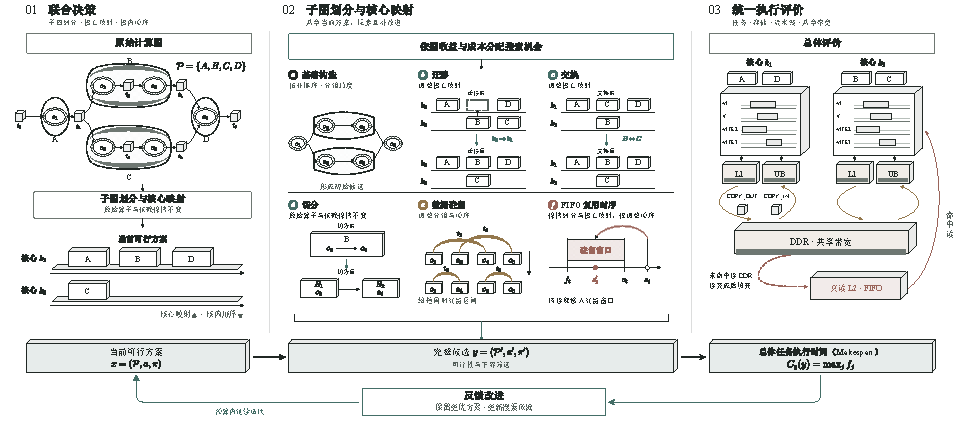
\includegraphics[width=\textwidth]{图片/workflow_qinglu_v7.pdf}
\caption{联合决策、多邻域候选与统一执行评价}\label{fig:roadmap}
\end{figure}

图~\ref{fig:roadmap} 以子图划分 $\mathcal P$、核心映射 $a$ 和核内顺序 $\boldsymbol\pi$ 表示完整方案 $x=(\mathcal P,a,\boldsymbol\pi)$。环节01保存当前可行方案；环节02构造候选；环节03按任务、存储、流水线和带宽约束重建执行过程。评价结果用于保留更优方案，并调整后续候选来源的搜索机会。

环节02展开六种操作：基础构造（a）按拓扑序和分组粒度产生初值；迁移（b）改变一个完整子图的所属核心；交换（c）对调不同核心上的子图；切分（d）将子图分成更细单元，保留原算子及依赖；数据驻留调整（e）通过分组与顺序缩短同时存活的数据区间；FIFO时序调整（f）移动已有子图，使后续读入有机会落入缓存驻留窗口。第一问使用（a）--（d），第二问增加（e），第三问进一步增加（f）。其中（b）--（d）同属结构与负载来源，六种操作围绕同一完整方案交替提出候选。

右侧示意各核心的私有L1、UB与共享DDR。第三问增加只读L2：发射读请求时查询缓存，命中由L2服务，未命中由DDR服务；读完成后按容量条件尝试填充。图中 $f_t$、$e_t$ 是张量 $t$ 的填充和淘汰时刻，$s_t,s'_t$ 是调整前后的读取时刻。新方案会改变这些时刻，故每个候选均通过完整执行评价。评价首先比较总体任务执行时间，周期相同时再比较总额外数据搬运量；搜索结束输出当前方案，第三问再固定该方案进行无L2与有L2配对。

\GMCMChapterEnd{1}
\section{模型假设}

本题给出的计算图、硬件配置与评估程序构成模型的既定条件。计算图中的张量大小、核内计算周期、依赖方向和输入输出位置固定；方案只决定非边界搬运算子的子图归属、子图的核心分配以及每核的子图顺序。原始边界搬运、跨任务交接、容量不足时的换出与取回、流水线占用和共享带宽竞争均按题目规定生成与评价。下列条件分别明确题设执行规则和理论推导的适用范围。

\begin{enumerate}
  \item \textbf{题设执行条件。} 给定同构核心数、私有L1和UB容量及DDR总带宽；场景A与场景B的执行任务组成和等待规则分别固定，第三问另有独立带宽的只读L2。对同一问题、图与配置，所有候选均交由同一官方评估语义判定可行性和完成周期。该条件使不同方案在相同的换出策略、缓存替换和流水线服务规则下比较。
  \item \textbf{固定工作量条件。} 在理论下界的计算部分，将原图中每个待执行计算算子的题给服务周期视为非负且不可省略，并保留其必需的数据依赖。所有合法方案均保留这部分工作量。该条件用于计算路径和每种计算流水线的工作量松弛；实际完成时间仍包含题定搬运、等待和资源争用。
  \item \textbf{必要流量的条件使用。} 只有在某些字节对全部合法方案都必须由DDR服务，且初始缓存状态、逻辑张量别名和输出要求均支持这一判断时，才把这些字节计入全局DDR服务下界。可由只读L2服务的读取按实际服务路径单独分析。必要流量用于下界证明和停止判据，额外COPY则按题定口径统计。
\end{enumerate}

通信量与片上活跃集估计用于候选排序；容量可行性、Spill数量、缓存命中和总体任务执行时间（Makespan）由完整执行评价确定。各问的经验结果均以其对应问题和配置的实际评估响应为准。


\GMCMChapterEnd{2}
\section{关键性符号说明}

贯穿三问的主要符号见表~\ref{tab:key-symbols}。局部事件变量与算法参数在首次使用处定义。
\begin{GMCMSymbolTable}{本表列出贯穿三问的公共符号，局部事件变量及算法参数在正文首次出现处定义。}
\GMCMSymbolRow{图}{G}{原始张量—操作二部有向计算图，$G=(T\cup O,E)$}{—}
\GMCMSymbolRow{集合}{T}{原始计算图的张量节点集合}{—}
\GMCMSymbolRow{集合}{O}{原始计算图的操作节点集合，含边界搬运操作}{—}
\GMCMSymbolRow{集合}{E}{张量与操作之间的有向依赖边集合}{—}
\GMCMSymbolRow{集合}{V}{待分配的非\texttt{COPY\_IN}/\texttt{COPY\_OUT}算子集合}{—}
\GMCMSymbolRow{集合}{K}{可用同构核心的集合，$K=\{1,\ldots,n\}$}{—}
\GMCMSymbolRow{参数}{n}{当前配置的核心数}{核}
\GMCMSymbolRow{参数}{b_t}{张量$t$的大小}{B}
\GMCMSymbolRow{参数}{p_v}{计算算子$v$的题给服务周期}{周期}
\GMCMSymbolRow{参数}{B_r}{片上存储区$r$的容量，$r\in\{L1,UB\}$}{B}
\GMCMSymbolRow{参数}{\beta_{\mathrm{DDR}}}{所有核心共享的DDR总服务带宽}{B/周期}
\GMCMSymbolRow{参数}{\beta_{\mathrm{L2}}}{第三问只读L2的独立读服务带宽}{B/周期}
\GMCMSymbolRow{变量}{\mathcal P}{待分配算子的非空互斥子图划分}{—}
\GMCMSymbolRow{变量}{a}{子图到核心的映射}{—}
\GMCMSymbolRow{变量}{\boldsymbol\pi}{各核心的子图执行顺序组成的序列族}{—}
\GMCMSymbolRow{变量}{x}{由划分、归核和核内顺序构成的完整方案，$x=(\mathcal P,a,\boldsymbol\pi)$}{—}
\GMCMSymbolRow{指标}{C_q(x)}{问题$q$中方案$x$的总体任务执行时间（Makespan）}{周期}
\GMCMSymbolRow{指标}{D_q(x)}{问题$q$中方案$x$的官方总额外COPY字节量}{B}
\GMCMSymbolRow{界}{L}{对当前问题全部可行方案成立的周期下界}{周期}
\GMCMSymbolRow{界}{U}{当前已验证可行方案的完成周期}{周期}
\end{GMCMSymbolTable}


\GMCMChapterEnd{3}
\section{问题一求解与分析}
\label{sec:q1}
\subsection{问题的描述与分析}
每个子图均作为一个独立执行任务。子图划得过细，虽然容易将计算量分散到多个核心，却增加了任务切换和跨子图搬运；子图过大，又可能压低并行度，并加剧片上存储压力。因此，子图划分、核心归属和核内子图顺序应联合决定。本文用一个完整方案描述三项决策，再以固定执行规则得到总体任务执行时间。后两问保持这一决策空间，通过改变任务边界、交接和缓存规则，解释同一类方案的执行差异。

图~\ref{fig:q1_overview} 概括本问的求解逻辑。先从原始计算图提取依赖、计算负载和张量复用关系，形成若干完整初始方案；再围绕当前可行方案进行互补的邻域改进。计算开销较低的结构预检和下界用于筛选候选，完整执行评价决定是否保留候选。最后从核数扩展、逐例差异、搜索过程和目标界四个方面分析结果。
\begin{figure}[htbp]
\centering
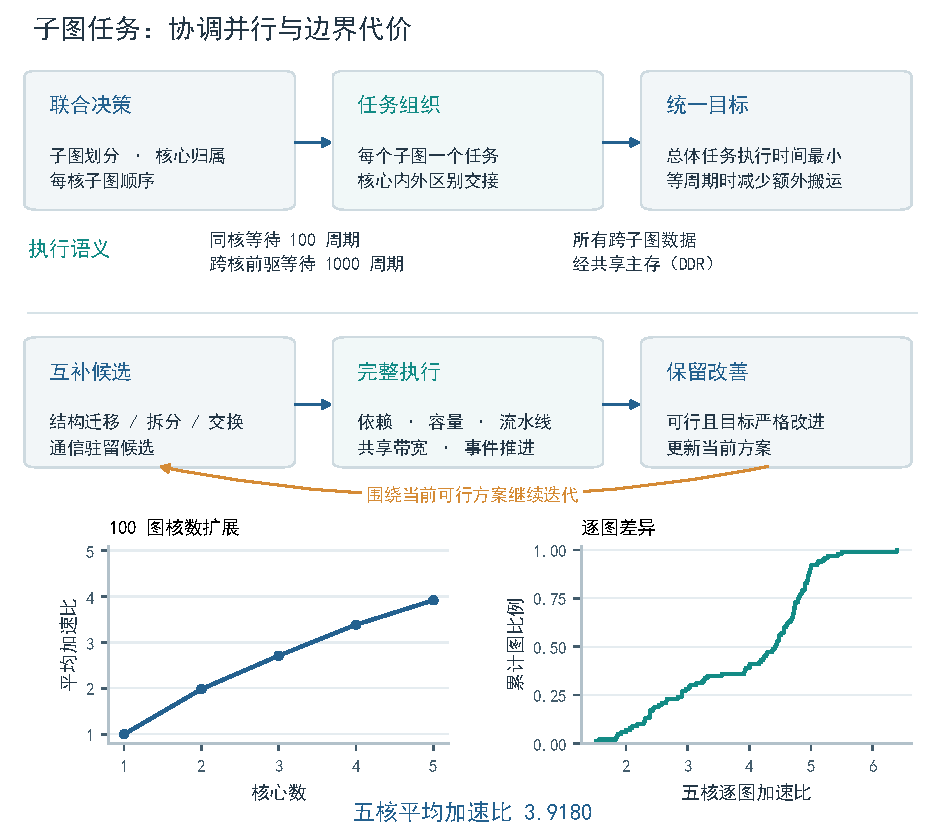
\includegraphics[width=\textwidth]{../求解/问题一/图片/q1_overview.pdf}
\caption{问题一的联合建模与迭代改进框架}\label{fig:q1_overview}
\end{figure}


\subsection{联合决策模型与统一目标}
\subsubsection{计算图、张量与划分}
原始二部有向无环图记为 $G=(T\cup O,E)$，其中 $T$ 为张量集合，$O$ 为操作集合。定义需要分配的非边界搬运算子集合
\begin{equation}
 V=\{o\in O:\operatorname{type}(o)\notin\{\mathrm{COPY\_IN},\mathrm{COPY\_OUT}\}\},
\end{equation}
\noindent 式中，$\operatorname{type}(o)$ 为操作类型，$\mathrm{COPY\_IN}$ 和 $\mathrm{COPY\_OUT}$ 分别表示核外数据搬入与搬出。模型保留原始算子的类型与计算周期、张量大小和依赖关系，再按任务划分及执行规则重建边界搬运操作。对于张量 $t\in T$，记其大小为 $b_t$，生产者与消费者集合分别为 $P_t$ 和 $C_t$。同一张量的多个消费者共享其生产关系，因而具有潜在的数据复用机会。生产者到多个消费者的关系可用有向超边表达；相关无环超图划分研究提供了这种集合表示\cite{A39}。本文仍依据任务边界生成实际搬运，候选中的通信排序量按相关张量字节构造，不以超边连接度替代实际搬运量。

设可用核心集合为 $K=\{1,\ldots,n\}$。完整方案写为
\begin{equation}
 x=(\mathcal P,a,\boldsymbol\pi),\qquad
 \mathcal P=(V_1,\ldots,V_m),\quad a:\{1,\ldots,m\}\longrightarrow K ,
 \label{eq:plan}
\end{equation}
\noindent 式中，$m$ 为子图数，$\boldsymbol\pi=(\pi_1,\ldots,\pi_n)$；$V_i$ 是第 $i$ 个子图包含的算子集合，$a(i)$ 是该子图的核心归属，$\pi_k$ 是核心 $k$ 上子图的执行顺序。划分满足
\begin{equation}
 V_i\ne\varnothing,\qquad \bigcup_{i=1}^{m}V_i=V,\qquad
 V_i\cap V_j=\varnothing\quad(i\ne j).
 \label{eq:partition}
\end{equation}
每个子图恰好出现于一个核心序列且只出现一次，允许部分核心没有子图。核数增大扩展了可用资源和方案选择空间，具体使用的核心数由方案决定。

将各 $V_i$ 收缩为顶点，可得到子图依赖商图 $H(\mathcal P)$。再加入各 $\pi_k$ 中相邻子图的顺序边，得到 $H_x$。必要条件为
\begin{equation}
 H_x\text{ 是有向无环图}.
 \label{eq:acyclic}
\end{equation}
无环性需要在收缩后重新检查。例如，交错地收集依赖链上不连续的算子，可能在商图中产生双向依赖。无环划分文献对此给出了明确约束\cite{A02}。执行中还存在执行流水线和存储复用关系，所以式~\eqref{eq:acyclic} 用于结构筛选，最终可行性由完整执行确定。

\subsubsection{执行映射与三问的共同方案空间}
记固定配置为 $\theta$，问题编号为 $q\in\{1,2,3\}$。定义执行映射
\begin{equation}
 \mathcal E_q(G,x;\theta)
 =\bigl(\operatorname{feas}_q(x),\mathcal R_q(x),C_q(x),D_q(x)\bigr),
 \label{eq:evaluator}
\end{equation}
\noindent 式中，$\operatorname{feas}_q(x)\in\{0,1\}$ 表示可行性，$\mathcal R_q(x)$ 为完整执行事件序列，$C_q(x)$ 为总体任务执行时间，$D_q(x)$ 为总额外数据搬运量（额外COPY字节）。对于重建边界搬运、插入存储换出和取回后得到的操作集合 $J_q(x)$，设操作 $j$ 的开始、完成时刻为 $s_j,f_j$。定义
\begin{equation}
 C_q(x)=\max_{j\in J_q(x)} f_j,
 \qquad x\in\mathcal F_q:=\{x:\operatorname{feas}_q(x)=1\},
 \label{eq:makespan}
\end{equation}
\noindent 式中，$\mathcal F_q$ 为完整执行可行的方案集合，$C_q$ 以时钟周期计，$D_q$ 以字节计。本文以 $C_q$ 为主目标，周期相同则选择 $D_q$ 较小者，即
\begin{equation}
 \min_{x\in\mathcal F_q}^{\mathrm{lex}}\bigl(C_q(x),D_q(x)\bigr),
 \label{eq:objective}
\end{equation}
\noindent 式中，$\mathrm{lex}$ 表示字典序比较。总额外数据搬运量等于调度后逻辑COPY总字节减去原图已有COPY字节，包含重建边界搬运与缓存换入换出。若读请求命中L2，则改由L2服务，但仍保留相应逻辑COPY操作；实际DDR服务字节另按请求的服务路径统计。

三问均采用式~\eqref{eq:plan} 的决策，改变的是执行映射。记算子 $v$ 所属子图为 $g(v)$，其执行任务标识为
\begin{equation}
 \chi_q(v)=\begin{cases}g(v),&q=1,\\a(g(v)),&q=2,3.\end{cases}
 \label{eq:task}
\end{equation}
这一定义把三问组织为同一模型的三个执行场景：第一问任务随子图划分，第二问任务随核心划分，第三问在第二问基础上增加共享只读缓存。三项决策通过各自的执行规则共同影响同一个优化目标。

\subsection{第一问的执行、存储与带宽约束}
\subsubsection{任务边界与交接}
一个子图对应一个Task。同一核心相邻任务之间也需要把边界张量写入 DDR，下一任务再读取，因此同核任务边界也产生搬运代价。任务聚类研究中的分组思想\cite{A49}需在这一边界条件下使用。图~\ref{fig:q1_task} 表示第一问的任务边界与就绪关系。
\begin{figure}[htbp]\centering
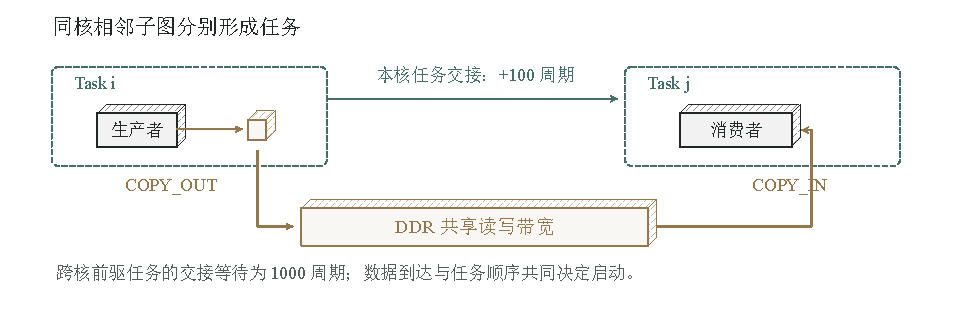
\includegraphics[width=\textwidth]{../求解/问题一/图片/q1_task.pdf}
\caption{子图级任务的边界与交接}\label{fig:q1_task}
\end{figure}

设任务 $i$ 的启动、完成时刻分别为 $S_i$ 和 $F_i$。任务 $j$ 的启动须同时满足其数据依赖和本核前序任务约束。对相邻本核任务，须有 $S_j\ge F_i+100$；对跨核前驱任务，须有 $S_j\ge F_i+1000$。存在多个前驱时，启动时刻受这些约束的最大值限制。100 与 1000 均以周期计，搬运本身占用的共享 DDR 服务时间还需单独通过事件执行获得。

任务边界使粒度选择出现双重影响。合并子图可以消除两者之间的一部分任务切换和边界搬运，但也固定了更多算子的共同归核，减少跨核重叠机会。进一步合并还可能延长张量驻留区间，引发自动换出。粒度选择因而需要同时考虑边界搬运、计算并行与容量压力。

\subsubsection{固定核内调度与片上容量}
每核具有矩阵、向量、读入和写出四条流水线（Pipe）。每条流水线同时至多服务一个操作；不同流水线可以在满足依赖和容量条件时重叠。算子的开始时刻满足前驱完成、所属流水线可用以及所需片上缓冲可分配等条件。固定核内处理先给出固定操作顺序，再处理存储换出，最后生成流水线依赖。本文的决策作用于子图划分、归核和核内子图顺序。

令 $r\in\{\mathrm{L1},\mathrm{UB}\}$ 表示片上存储区，$B_r$ 为容量；$\mathcal B_{k,r}(\xi)$ 是执行时刻 $\xi$（周期）核心 $k$ 在该区已分配且尚未释放的缓冲实例集合。容量条件写为
\begin{equation}
 \sum_{b\in\mathcal B_{k,r}(\xi)}\operatorname{size}(b)\le B_r,
 \quad B_{\mathrm{L1}}=524288\ \mathrm B,\quad B_{\mathrm{UB}}=131072\ \mathrm B,
 \label{eq:capacity}
\end{equation}
\noindent 式中，$\operatorname{size}(b)$ 为缓冲实例 $b$ 占用的字节数。一个逻辑张量在不同核上的驻留副本分别占用相应核心的容量。任务切换还会清除本核任务私有存储，跨任务复用必须经由规定路径完成。

在固定顺序下容量不足时，执行规则依据下一次使用位置选择允许换出的张量，并在后续需要时重新取回。当前操作需要的输入、输出等对象受换出资格限制。换出与取回属于执行映射；调整划分和顺序可能改变其发生位置及搬运量。联合调度与存储优化研究揭示了驻留状态与片外访问之间的联系\cite{A16}。本文据此分析活跃集和驻留压力，在固定分配与换出规则下提出划分和顺序候选。

\subsubsection{共享 DDR 的事件推进}
设 DDR 总带宽为 $\beta_{\mathrm{DDR}}=60\ \mathrm B/\text{周期}$。对当前在途 DDR 读写请求集合 $\mathcal A_D(\xi)$，记 $m_D(\xi)=|\mathcal A_D(\xi)|$。若以独占该带宽所需周期表示请求 $j$ 的剩余服务量 $w_j$，在没有新的发射或完成事件的时间区间内，有
\begin{equation}
 w_j(\xi+\Delta)=\max\left\{0,w_j(\xi)-\frac{\Delta}{m_D(\xi)}\right\},\quad j\in\mathcal A_D(\xi),
 \label{eq:bandwidth}
\end{equation}
\noindent 式中，$\Delta$ 为在途集合不变的事件间隔，$m_D(\xi)>0$；$w_j$ 与 $\Delta$ 均以周期计。请求初始独占服务量按字节数除以带宽向上取整，且至少为1周期。新的读写发射、请求完成和任务就绪都会改变下一个事件时刻。事件执行依次处理完成事件，释放依赖和存储，再发射满足条件的新操作。

改变子图边界或归核即使减少了搬运字节，也可能使请求更集中，从而延迟关键计算链。第4.5节给出各来源的内部排序量；所有候选的正式周期均按上述事件过程计算。

\subsection{下界、候选过滤与质量界}
\subsubsection{对全体方案有效的下界}
取所有可行方案都保留的计算依赖图 $G_c$，其中算子 $v$ 的固定服务周期为 $p_v$，计算流水线类型为 $\rho(v)$。定义计算路径、流水线负载和必要 DDR 流量下界：
\begin{align}
 L_{\mathrm{path}}&=\max_{P\text{ 为 }G_c\text{ 中依赖路径}}\sum_{v\in P}p_v,\\
 L_{\mathrm{load}}&=\max_r\frac{\sum_{v:\rho(v)=r}p_v}{n},\\
 L_{\mathrm{DDR}}&=\frac{B_{\mathrm{mandatory}}}{\beta_{\mathrm{DDR}}},\qquad
 L=\max\{L_{\mathrm{path}},L_{\mathrm{load}},L_{\mathrm{DDR}}\},
 \label{eq:lower}
\end{align}
\noindent 式中，$r$ 遍历计算流水线类型，$B_{\mathrm{mandatory}}$ 只包含能证明所有方案都必须通过 DDR 服务的字节。对第一、二问，初始输入读取和最终输出写出提供这种必要流量；第三问的初始缓存为空，无逻辑别名时首次读取仍须经过 DDR。存在显式逻辑别名时，第三问的流量下界仅计必要写出量。

\textbf{命题1：}在计算依赖保留、算子不重算或删除、同类计算流水线每核串行、必要 DDR 流量判断成立的条件下，对任意可行方案 $x$，有 $L\le C_q(x)$。

\textbf{证明：}同一计算依赖路径上的算子只能依次完成，故执行周期不小于任意路径的计算服务量之和。每种计算流水线在 $n$ 个核心上的总能力为每周期至多提供 $n$ 个流水线周期，因此其总工作量除以 $n$ 不大于执行周期。DDR 在任意长为 $C_q(x)$ 的区间内至多服务 $\beta_{\mathrm{DDR}} C_q(x)$ 字节，必要流量又给出第三项约束。三项分别给出有效下界，取最大值仍成立；计算与搬运可以重叠，因此这里不将三项相加。证毕。

\subsubsection{固定候选的下界}
固定完整候选 $x$ 后，归核已经确定，可进一步计算每个核心各类流水线的工作量下界。第一问还可以在任务依赖和核心顺序合图上，按每个任务的计算负载下界及对应交接等待递推最早完成下界。设任务 $i$ 的工作下界为 $\ell_i$，前驱集合为 $\operatorname{pred}_x(i)$，交接等待为 $d_{hi}$，则
\begin{equation}
 z_i=\ell_i+\max_{h\in\operatorname{pred}_x(i)}(z_h+d_{hi}),
 \label{eq:taskbound}
\end{equation}
\noindent 式中，$z_i$ 为任务 $i$ 的完成时刻下界；无前驱时最大项取零。$\ell_i$ 取该任务各计算流水线总负载的最大值，允许流水线充分重叠；$d_{hi}$ 只使用规定的任务等待。由拓扑序归纳可知，真实任务完成时刻不早于 $z_i$。把这些项以及固定任务边界产生的必要搬运下界取最大值，得到候选专属下界 $L(x)$。

\textbf{命题2：}若 $L(x)\le C_q(x)$，当前已保留方案周期为 $U$，则 $L(x)>U$ 的候选不能改善主目标。

\textbf{证明：}$C_q(x)\ge L(x)>U$，故该候选的周期严格更差。证毕。过滤使用严格大于；当 $L(x)=U$ 时，候选仍可能在相同周期下减少额外 COPY 字节。候选下界刻画固定 $x$ 的周期约束；全局质量界使用对全部方案成立的 $L$。

\subsubsection{可行上界与相对差距}
令 $C_q^*$ 为全局最优周期，当前可行周期为 $U$。当 $0<L\le C_q^*\le U$ 时，
\begin{equation}
 0\le\frac{U-C_q^*}{U}\le1-\frac{L}{U},\qquad
 0\le\frac{U}{C_q^*}-1\le\frac{U}{L}-1,
 \label{eq:gap}
\end{equation}
\noindent 式中，第一组不等式以当前周期为分母，量化仍可能减少的比例；第二组不等式以最优周期为分母，量化当前解的相对超额。本文以第一式右侧作为近界停止依据，当其不超过 $0.0025$ 时停止继续改进。其他停止条件见算法~\ref{alg:joint}。

\subsection{多邻域迭代改进算法}
\subsubsection{初始构造与当前可行方案}
已有同配置方案经有效执行结果确认后可作为初值；否则由下述构造产生候选。构造时取 $\widetilde p_v=\max\{1,p_v\}$，设 $w_r(A)=\sum_{v\in A:\rho(v)=r}\widetilde p_v$，$W(A)=\max_r w_r(A)$。从算子依赖图的弱连通分量出发，依次切分负载最大的分量。对固定拓扑序的非空前缀 $A$ 和后缀 $B$，切点按
\begin{equation}
 \min_{A\dot\cup B=V_i}
 \left[\max\{W(A),W(B)\}+\gamma_q F(A,B)/\beta_{\mathrm{DDR}}\right],
 \quad \gamma_1=2,\quad\gamma_2=\gamma_3=1,
 \label{eq:frontier_construct}
\end{equation}
\noindent 式中，$F(A,B)$ 是在两侧均有生产或消费操作的张量字节总和；每个张量只计一次。该量用于切点排序，不是总额外数据搬运量。长度大于6时只考察位置比例为15\%--85\%的切点；并列时先取负载差较小者，再取较早切点。切开后分别取两侧弱连通分量。对粒度 $g\in\{2,4,8\}$，当最大块负载不超过 $\max\{1,W(V)/(gn)\}$ 或已切分 $2gn$ 次时结束该构造。

给定划分后，以算子上行优先级 $r_v=\widetilde p_v+\max_{u\in\operatorname{succ}(v)}r_u$（无后继时最大项为0）的块内最大值，在就绪子图中选取优先级最高者。对待放置子图 $i$，计算各核的估计完成位置
\begin{equation}
 \widehat E_i(k)=\max_r\{\max(\ell_{k,r},R_i(k))+w_r(V_i)\},\qquad
 a(i)=\mathop{\arg\min}_{k\in K}^{\mathrm{lex}}
 \left(\widehat E_i(k)+\frac{Q_i(k)}{4\beta_{\mathrm{DDR}}},\max_r\ell_{k,r},k\right),
 \label{eq:construct_map}
\end{equation}
\noindent 式中，$\ell_{k,r}$ 为已安排子图在核 $k$、流水线 $r$ 上的估计负载位置；$R_i(k)$ 为前驱估计完成时刻加交接等待后的最大值，空前驱取0。交接等待在第一问取同核100、跨核1000周期，在后两问取同核0、跨核500周期。$Q_i(k)$ 为子图外部输入字节：第一问全部计入，后两问扣除此前已给核 $k$ 分配过的输入张量。选中核心后将 $i$ 接至其序列末端；对 $w_r(V_i)>0$ 的流水线，令 $\ell_{k,r}\leftarrow\max\{\ell_{k,r},\widehat E_i(k)-W(V_i)\}+w_r(V_i)$，其余不变。

式~\eqref{eq:construct_map} 是上行优先级与最早完成时间（Earliest Finish Time，EFT）思想下的构造估计\cite{A01}，不等于共享带宽执行周期。还保留单前驱、单后继边连接的链分组，以及按依赖层宽度变化划分阶段的构造；同阶段同核心的块可合并。基础来源同时探索不同阶段粒度，结构来源探索链分组在不同有效核数和通信权重下的映射。分组与并行执行共同决定候选价值\cite{A08}，所有初值均用 $\mathcal E_q$ 确认。

\subsubsection{互补候选与完整方案更新}
记基础、结构、驻留和缓存时序来源分别为 $\mathrm B,\mathrm S,\mathrm M,\mathrm F$。基础候选 $\mathcal N_{\mathrm B}$ 包括前述多粒度构造，以及负载驱动的迁移、前沿切分和同核相邻子图交换。其部分候选按
\begin{equation}
 \widehat C_q(y)=\max\{\widehat C_{\rm time}(y),\widehat C_{\rm bus}(y)\}
       +\widehat D_{\rm spill}(y)/\beta_{\mathrm{DDR}},
 \label{eq:base_proxy}
\end{equation}
\noindent 式中，$\widehat C_{\rm time}$ 为简化时序估计，$\widehat C_{\rm bus}$ 为估计DDR/L2服务负载的最大值，$\widehat D_{\rm spill}$ 为活跃区间超容量量导出的换入换出字节估计。它们只用于该来源内排序；共同候选入口使用的是有效下界 $L(y)$，不将式~\eqref{eq:base_proxy} 用于证明性剪枝。

结构候选 $\mathcal N_{\mathrm S}$ 包含四种变换。取当前合图 $H_x$ 的拓扑序 $\sigma$，用 $\sigma|_A$ 表示只保留集合 $A$ 中子图的子序列。对选定子图集合 $A$ 及新归核 $\mu:A\to K$，定义
\begin{equation}
 a'(i)=\begin{cases}\mu(i),&i\in A,\\a(i),&i\notin A,\end{cases}
 \qquad \pi'_k=\sigma|_{\{i:a'(i)=k\}},\qquad
 y=(\mathcal P,a',\boldsymbol\pi'),
 \label{eq:group_move}
\end{equation}
\noindent 式中，$A=\{i\}$ 给出单子图迁移；$A=\{i,j\}$ 且互换两者归核给出跨核交换；令两者归至同一核给出联合迁移。前缀拆分则把 $V_i$ 的拓扑序在 $1/4,1/2,3/4$ 处截为两个非空块，保留前块归核，将后块放到负载较轻的另一核，再按 $\sigma$ 重建核序。大划分优先考察晚完成、高负载和高跨核通信子图；迁移组合按最大流水线负载变化加关联跨核字节变化除以DDR带宽排序。该关联字节量同样不是正式COPY指标。

驻留候选 $\mathcal N_{\mathrm M}$ 根据生产与消费关系重组完整子图。第一问特有的生产者释放切分针对长任务：对跨核张量 $t$ 在 $V_i$ 内的生产者，取其组内前驱闭包 $A$，令 $B=V_i\setminus A$。当两部分非空且
\begin{equation}
 F_i-\max_{v\in P_t\cap V_i}f_v>100,
 \label{eq:release_split}
\end{equation}
\noindent 式中，$F_i$、$f_v$ 分别是当前执行中任务与生产者的完成时刻。满足式~\eqref{eq:release_split} 时，将 $(A,B)$ 依次留在原核。按此时间差递减取至多4个候选，尝试提前释放跨核数据，同时仍须支付新增任务交接成本。后两问的驻留重组见算法~\ref{alg:residency}，第三问另增加算法~\ref{alg:fifo} 的纯顺序候选。

多初值与局部迁移共同组织搜索\cite{A42}。各来源均给出完整 $y$；在同配置完整评价后，统一更新为
\begin{equation}
 x^+=\begin{cases}
 y,&y\in\mathcal F_q\ \text{且}\ (C_q(y),D_q(y))<_{\rm lex}(C_q(x),D_q(x)),\\
 x,&\text{其他情形}.
 \end{cases}
 \label{eq:accept}
\end{equation}
接受后以 $(x^+,\mathcal R_q(x^+))$ 重建依赖当前解的局部候选；与当前解无关的构造继续给出尚未考察的方案。相同完整方案不重复评价。

\subsubsection{来源选择与有限预算}
候选生成和完整评价的成本差异较大，因此按近期反馈分配搜索机会。对第 $j$ 次调用，记评价前当前最好周期为 $U_j$，候选周期为 $C_j$，周期收益取 $g_j=\max\{0,1-C_j/U_j\}$；评价失败或周期持平时记零。设来源 $s$ 的近期收益均值为 $\bar g_s$，生成与评价总用时中位数为 $\widehat c_s$，失败比例为 $r_s$，已完成调用数为 $N_s$，所有来源的总调用数为 $N_{\rm call}$。在初次覆盖、可用性和剩余时间准入条件满足后，比较指数
\begin{equation}
 I_s=\frac{\bar g_s+0.012\sqrt{\log(2+N_{\rm call})/(1+N_s)}}{
 \max(0.005,\widehat c_s)(1+r_s)},
 \label{eq:sourcepriority}
\end{equation}
\noindent 式中，近期均值、中位数和失败比例按最近八次调用计算。前项奖励已观察到的改进，第二项为尚未充分尝试的来源保留机会，分母计入运行成本和失败倾向。搜索资源根据测量反馈分配的思路与程序自动调优中的经验一致\cite{A12}；式~\eqref{eq:sourcepriority} 将上述因素组合为启发式来源优先级。

初期优先选择已完成调用不足2次且已生成候选不足12个的来源。第三问仅在结构与驻留成功调用合计不足4次、且累计用时低于 $\min\{20,0.18\tau_{\max}\}$ 秒时暂缓缓存时序来源。其后优先选择距上次调用已隔至少8次的来源，否则比较式~\eqref{eq:sourcepriority}；准入成本为 $1.2\max\{0.005,\widehat c_s\}+0.05$ 秒，若已有调用记录且无来源能在剩余时间内完成，则停止。

每个图、问题及核数配置的累计主机时间上限 $\tau_{\max}=600$ 秒，评价上限为2048次；总时间包含解析、已有方案确认、候选生成、评价与保存，第三问的同方案配对在总预算内预留时间。近界、预算耗尽、来源耗尽或停滞均可终止搜索。停滞要求同时满足：至少30秒没有周期改善、连续至少32次评价未改善周期、每个仍可用来源至少8次未改善周期。仅次要指标改善可以接受，但不重置周期停滞条件。

\subsubsection{可行性保持与目标单调性}
\textbf{命题3：}若初始方案 $x^{(0)}\in\mathcal F_q$，每次只在相同配置下接受完整执行可行且字典序严格改善的候选，则所有已保留方案均可行，且目标序列字典序单调不增。

\textbf{证明：}初始方案可行。第 $k$ 步若没有接受新候选，则保留 $x^{(k)}$；若接受 $y$，其已通过完整执行且 $\bigl(C_q(y),D_q(y)\bigr)<_{\mathrm{lex}}\bigl(C_q(x^{(k)}),D_q(x^{(k)})\bigr)$，因此 $x^{(k+1)}=y$ 可行且严格改善。由归纳法得结论。证毕。

停止时，式~\eqref{eq:gap} 用有效全局下界与已取得的可行上界给出周期质量范围；有限预算停止不蕴含全局最优性。

\subsection{联合迭代的计算过程}
\subsubsection{从完整方案到一次可接受的改进}
第~\ref{sec:q1} 节给出了方案空间、全局下界和接受准则。本节把候选从生成到保存的计算顺序具体化。对一个固定的计算图、问题编号和核数，搜索状态包含已验证的当前最好方案 $x$、对应完整执行结果、父方案代号、已经评价或安全剪枝的完整方案集合，以及各候选来源的近期记录。各来源共享同一个当前最好状态。初始构造可以来自本配置下已经验证的完整方案，或由依赖关键性、阶段粒度与负载映射生成。对初始候选先做结构检查，再取得完整执行结果；只有合法结果才进入当前最好状态。

一次迭代可按下列顺序表述，其中 $U=C_q(x)$，$L(y)$ 是固定候选 $y$ 的有效周期下界：
\begin{enumerate}
  \item 根据仍可用的来源、近期改善幅度、生成与评价成本、失败比例及剩余时间选择一个来源。初次覆盖和久未访问的来源获得机会；预计成本超过剩余时间时停止准入。
  \item 来源提出完整候选 $y=(\mathcal P',a',\boldsymbol\pi')$。检查非边界算子覆盖、每个子图恰有一次归核及商图与核内顺序合图的无环性；相同完整方案不重复评价。
  \item 若 $L(y)>U$，该候选不可能改善主目标，直接筛去。等号情形保留，因为周期持平时额外 COPY 字节仍可能下降。
  \item 对其余候选调用完整执行，重建任务和边界搬运、自动换出、Pipe 排布与共享带宽事件。只有结果可行，且 $(C_q(y),D_q(y))<_{\rm lex}(C_q(x),D_q(x))$，才令 $x\leftarrow y$ 并更新父方案代号；取得的解在评价和保存完成后才计为可用。
  \item 检查全局下界相对差距、评价次数、墙钟预算、来源耗尽和停滞条件。第三问结束主搜索后，对已选同一方案另作无缓存评价，配对结果不参与主搜索的接受判断。
\end{enumerate}
选择来源的反馈指数见式~\eqref{eq:sourcepriority}。实际准入先覆盖少量可用来源并检查时间可行性，再依据近期收益和成本分配评价机会。每次接受都会改变父方案，故候选生成必须明确绑定接受前的状态。例如驻留候选使用先前的张量生命周期，缓存候选使用先前的读入与淘汰事件；若父方案改变，继续消耗旧候选流可能把旧事件错误关联到新划分或新归核。实现因此在新父方案代号出现后重建依赖父方案的结构、驻留和缓存流，并以已接受的完整方案及执行记录为起点。与父方案无关的全局构造流则保存其迭代位置，避免每次改进后重新生成相同初值。各来源由此围绕同一方案持续衔接。

\subsubsection{邻域更新、结构预检与计算量}
令 $N=|V|$ 为需归组的非边界算子数，$M$ 为这些算子间保留的依赖边数，$m$ 为当前子图数，$H(y)$ 为候选 $y$ 的完整执行实际处理的事件数。一次“迁移”把一个完整子图从原核心序列删除，再插入目标核心序列的某个合法位置；它更新 $a$ 与相关的 $\pi_k$，但不改变该子图内部算子集合。“交换”改变两个子图在一个或两个核心序列中的相对位置；若跨核交换，还同时更新两者归属。“拆分”把某子图分成非空、互不相交的两部分，在算子到子图映射中为新部分赋编号，并重新安置两部分的核心位置与先后顺序。联合迁移及张量关联移动按依赖闭合的子图集合操作，其输出仍须含全部 $N$ 个算子的完整映射和各核序列。拆分后的新增边界搬运、迁移后的跨核通信以及顺序变化造成的驻留区间，均由新方案的完整执行重新计算。

给定一个已经构造好的完整候选，扫描 $N$ 个算子建立组成员与归属，扫描 $M$ 条依赖建立跨组前驱，再加入各核相邻子图的顺序边。后者总数不超过 $m$；在合图上做一次拓扑检查，按通常邻接表实现，其工作量为 $O(N+M+m)$，存储量同阶。这是结构预检的计算量。环检查能够排除“某组必须先于另一组、又被核内顺序要求后于另一组”的矛盾，却不能决定瞬时缓冲是否可分配、自动换出是否引入额外请求、任务等待如何落在时间轴上，以及共享带宽在并发请求间如何分配。因此，通过预检的候选仍须完整执行验证。对事件评价记其实际成本为 $T_{\rm eval}(N,M,m,H(y))$；该成本随操作数量、事件数量及并发请求的重排共同变化。

候选空间本身也远大于一次预检。只枚举单个子图向其他核心迁移，已有至多 $m(n-1)$ 种归核选择；再考虑每个目标核心的插入位置、两个子图交换、组内依赖合法的拆分、多个关联组联动，候选数会继续增加。完整执行还有固定方案生成的 COPY、Spill 和 FIFO 事件，$H(y)$ 由候选的实际轨迹决定。实际程序对单次来源流设生成上限，整配置最多评价 $2048$ 次，并以 $600$ 秒总预算及剩余时间准入约束搜索。若实际完成 $B$ 次评价，总代价应写成各次生成、结构检查、保存及 $\sum_{i=1}^{B}T_{\rm eval}(N,M,m_i,H_i)$ 的和。下界剪枝、去重和早停共同减少实际调用。

\subsubsection{两张五核图的方案展开}
真实五核方案能够说明“子图数”与“执行任务数”在两问中的差别。算例080在第一问选出 $3$ 个子图，核心序列长度为 $(1,1,1,0,0)$：五个核心可用，但只有三个核心承担工作，三个子图分别构成 Task，最终总体任务执行时间为 $100325$ 周期，额外 COPY 为 $3047424$ B。第二问对同图独立寻优后得到 $161$ 个子图，五核序列长度为 $(34,32,34,30,31)$，周期为 $71369$，额外 COPY 为 $2273280$ B。第二问仍有许多子图，却只有五个核心级 Task；同核子图可延续存储状态，跨核交接按写出完成后等待的规则执行。两问的任务边界与所选划分、归核和顺序共同产生了这组周期差异。

算例046的第一问五核方案含 $15$ 个子图，序列长度为 $(4,2,2,2,5)$。每个子图是独立 Task，所以五核序列中共有 $15-5=10$ 处同核相邻 Task 交接；承担五个子图的核心至少经历四次按题设定义的相邻任务等待。该方案周期为 $91730$，额外 COPY $3669568$ B，其中划分搬运 $3564096$ B、自动换出 $105472$ B。第二问独立选出的方案含 $31$ 个子图，序列长度为 $(5,7,7,5,7)$，周期 $69268$，额外 COPY $2469536$ B，未产生自动换出的额外字节。第二问的更多子图仍属于五个核心级Task。同核任务等待、跨核依赖和DDR服务在五核执行中相互交错，周期由完整事件序列决定。两例分别展示了有效核心数、子图粒度和自动换出如何与任务规则共同进入完整周期。

\subsubsection{可行方案空间的嵌入性质}
现有下界说明任一可行结果距离全局最优最多仍可能改善多少。另有一项与核数有关、但不依赖搜索启发式的性质。固定问题编号和全部硬件参数，设允许核心空闲，增加一颗核心不减少原核心的 Pipe、L1/UB 容量，也不改变共享 DDR 或 L2 总带宽与事件优先规则。对任意 $n$ 核可行方案 $x$，构造 $n+1$ 核方案 $\iota(x)$：保持全部子图集合、算子映射、原有核心归属及原核序列不变，仅令新增核心的序列为空。由于没有任何新操作、COPY 或缓存请求从空核心发射，原方案的任务边界、缓冲实例和事件顺序均不变，故
\begin{equation}
 \iota(x)\in\mathcal F_q(n+1),\qquad
 C_q(\iota(x))=C_q(x),\qquad D_q(\iota(x))=D_q(x).
 \label{eq:core_embedding}
\end{equation}
于是同配置、同评价规则下的理论最优周期满足 $C_{q,n+1}^{*}\le C_{q,n}^{*}$。证明只需把任意 $n$ 核可行方案按上法嵌入 $n+1$ 核可行集；后者的最小值不大于其中这个方案的周期。该性质说明理论最优周期随核数增加单调不增。有限预算下，各核数的来源准入、候选顺序和搜索截止可能不同，实际选出方案的周期仍可能波动。第一、二问的一核点采用原始整图参考，其定义见式~\eqref{eq:speedup}。


\subsection{实验指标与第一问结果}
\subsubsection{统一评价与核数扩展}
实验使用题面提供的 100 个计算图及固定参数，统一以周期评价。算例编号与原始文件对应，例如算例080对应 \texttt{case\_080}。对算例 $i$，记原始整图单核周期为 $T_{i,0}$，问题 $q\in\{1,2,3\}$、$n$ 核方案周期为 $C_{i,q,n}$，定义
\begin{equation}
 S_{i,q,n}=\frac{T_{i,0}}{C_{i,q,n}},\qquad
 \overline S_{q,n}=\frac{1}{100}\sum_{i=1}^{100}S_{i,q,n},
 \label{eq:speedup}
\end{equation}
\noindent 式中，$S_{i,q,n}$ 为逐图加速比，$\overline S_{q,n}$ 为100图的算术平均。第一、二问的一核点采用原始整图单核参考，令 $C_{i,1,1}=C_{i,2,1}=T_{i,0}$，相应加速比为1。第三问一核点使用其实际有L2方案周期。均值按式~\eqref{eq:speedup} 对100个逐例比值取算术平均，使每个算例具有相同权重。

% 由求解/规范化数据/combined/means.csv 生成；逐图加速比的算术平均。
\begin{table}[htbp]
\caption{问题一各核数逐图加速比统计}\label{tab:q1_mean}
\centering\normalsize
\setlength{\tabcolsep}{5pt}
\begin{tabular}{rrrrrr}
\toprule
核心数 & 样本数 & 平均加速比 & 中位加速比 & 最小加速比 & 最大加速比 \\
\midrule
1 & 100 & 1.0000 & 1.0000 & 1.0000 & 1.0000 \\
2 & 100 & 1.9832 & 1.9810 & 1.2445 & 3.6480 \\
3 & 100 & 2.7106 & 2.8440 & 1.4596 & 5.4659 \\
4 & 100 & 3.3852 & 3.7003 & 1.5139 & 6.3806 \\
5 & 100 & 3.9180 & 4.4227 & 1.5157 & 6.3928 \\
\bottomrule
\end{tabular}
\end{table}

图~\ref{fig:q1_mean} 和表~\ref{tab:q1_mean} 给出核数扩展结果。五核平均加速比为 $3.9180$，中位数为 $4.4227$。由四核增加至五核后，平均加速比继续提高，增量小于低核数阶段。依赖串行部分、任务交接和共享带宽是解释这一变化时需要考虑的执行约束。
\begin{figure}[htbp]\centering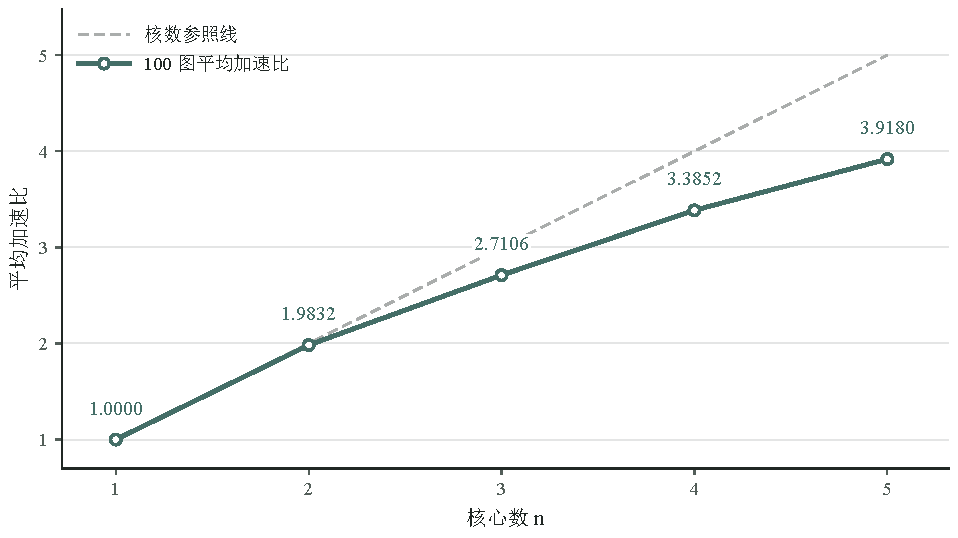
\includegraphics[width=.90\textwidth]{../求解/问题一/图片/q1_mean.pdf}
\caption{第一问各核数平均加速比}\label{fig:q1_mean}\end{figure}

\subsubsection{逐例分布及低收益图}
图~\ref{fig:q1_distribution} 展示二至五核加速比的经验分布。五核配置下，100 个图的加速比介于 $1.5157$ 与 $6.3928$，其中 6 个图低于 2，9 个图超过 5。均值低于中位数，说明少数低收益图对总体平均值有明显影响。
\begin{figure}[htbp]\centering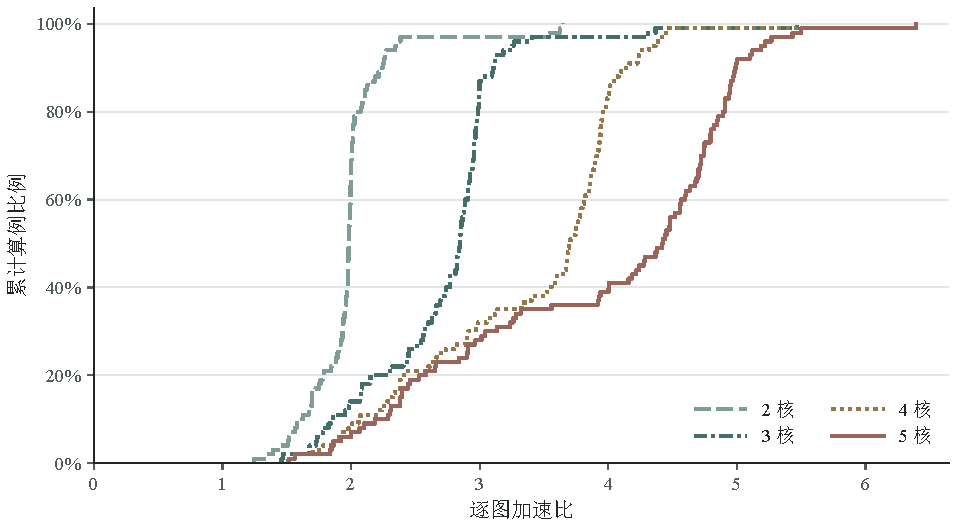
\includegraphics[width=.90\textwidth]{../求解/问题一/图片/q1_distribution.pdf}
\caption{第一问各核数加速比的逐例分布}\label{fig:q1_distribution}\end{figure}

与原始整图单核参考相比，多核方案还调整了分组和执行顺序，并可能改变自动换出与流水线重叠。该比较不只改变核心数，所以 $S=n$ 是参照线，加速比可以超过这一数值。低收益算例则需要结合计算依赖链、任务边界、负载分配和搬运争用分析。

本问五核额外 COPY 字节的均值为 $14585335.66$ B，中位数为 $1990466$ B，差异说明搬运规模具有明显长尾。88 个五核结果未产生自动换出的额外 COPY，其余12个结果呈现片上存储压力。

\subsubsection{任意时刻可用解与搜索过程}
搜索从同配置的已有可行方案或本次构造的初始候选出发。以下轨迹记录本次运行中完成评价和保存后可用的方案，不包含已有方案在此前运行中的生成用时；本次保存耗时计入可用时刻，跨过采点后才可用的解只进入后续采点。设 $\tau$ 为本次运行累计用时，$\mathcal A(\tau)$ 为在该时刻前已经完整评价并保存的可用候选集合。当该集合非空时，定义
\begin{equation}
 U(\tau)=\min_{x\in\mathcal A(\tau)}C_q(x).
 \label{eq:anytime}
\end{equation}
图~\ref{fig:q1_anytime} 以100个算例编号为纵轴、运行用时（秒）为横轴，每30秒采点。对算例 $i$，颜色表示当前可用周期相对最终周期的超额比例 $U_i(\tau)/C_{i,1,5}-1$，为无量纲量。30秒时93个算例取得可用解，其余位置留空。停止后若无新可用解，$U_i(\tau)$ 保持不变。
\begin{figure}[htbp]\centering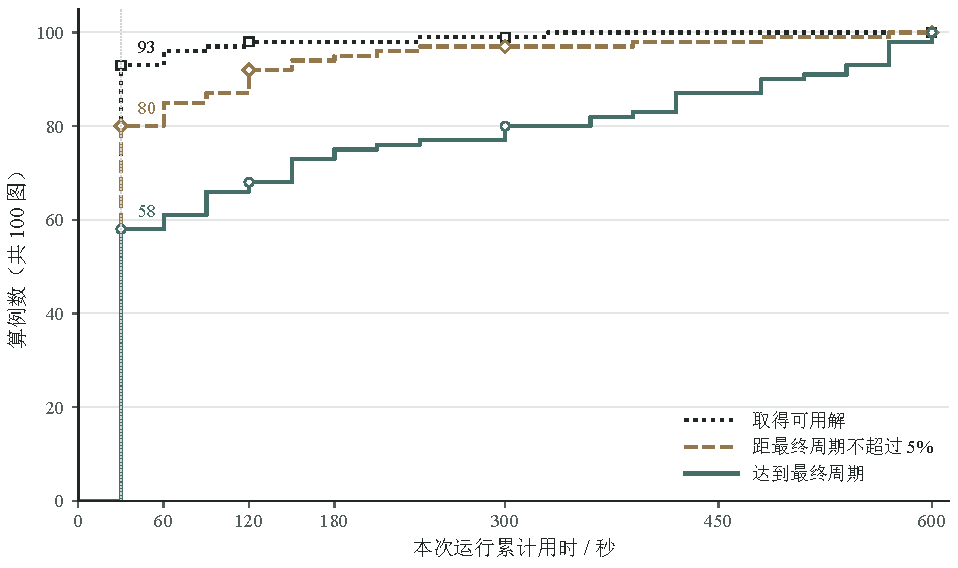
\includegraphics[width=\textwidth]{../求解/问题一/图片/q1_anytime.pdf}
\caption{第一问五核可用解的相对周期差距}\label{fig:q1_anytime}\end{figure}

\subsubsection{下界与结果解释}
图~\ref{fig:q1_bound} 对照五核结果周期及全局下界。下界接近结果时，继续搜索能够带来的相对周期减少受到式~\eqref{eq:gap} 约束；下界较松时，差距同时受方案质量和松弛程度影响，任务交接、容量与带宽竞争等未被充分刻画的约束也可能扩大该区间。
\begin{figure}[H]\centering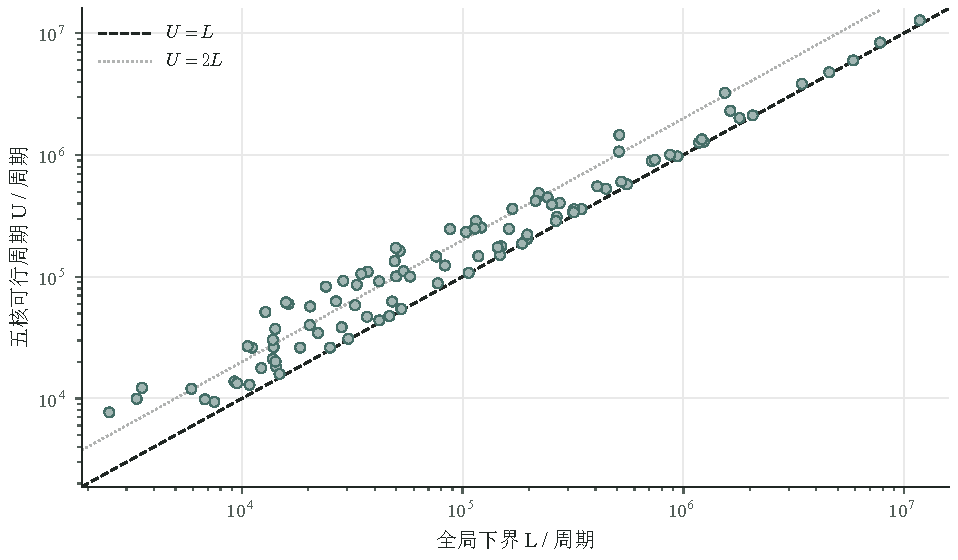
\includegraphics[width=.92\textwidth]{../求解/问题一/图片/q1_bound.pdf}
\caption{第一问五核可行周期与全局下界}\label{fig:q1_bound}\end{figure}

在这100个算例上，联合划分与调度取得了上述多核结果。第二问沿用决策和接受准则，将任务边界扩展到核心，考察同核片上驻留和跨核交接的变化。

\GMCMChapterEnd{4}
\section{问题二求解与分析}
\label{sec:q2}
\subsection{问题的描述与分析}
第二问延续第~\ref{sec:q1} 章的完整方案 $x=(\mathcal P,a,\boldsymbol\pi)$、总体任务执行时间 $C_q$ 和额外 COPY 字节 $D_q$，但重新界定执行任务：一个核心上的全部子图共同构成一个 Task。子图划分与核内顺序仍规定算子的归核、局部先后与跨核边界；改变的是同核子图之间的状态能否延续，以及跨核交接的就绪条件。同一张量若由本核的后续子图使用，可以继续占据 L1 或 UB，从而减少边界写回与重读。驻留时间延长也可能触发自动换出，形成搬运节省与容量压力之间的权衡。

图~\ref{fig:q2_overview} 给出本问的求解脉络。算法按核心级 Task 重建交接与内存生命周期，围绕跨核通信、驻留峰值和并行度提出候选，并沿用完整评价与字典序接受准则。结果分析同时观察五核加速比、与第一问的逐图周期比、额外 COPY 变化和候选来源记录。前两问各自独立寻优，逐图比较反映执行规则与方案选择共同作用后的表现。
\begin{figure}[htbp]
\centering
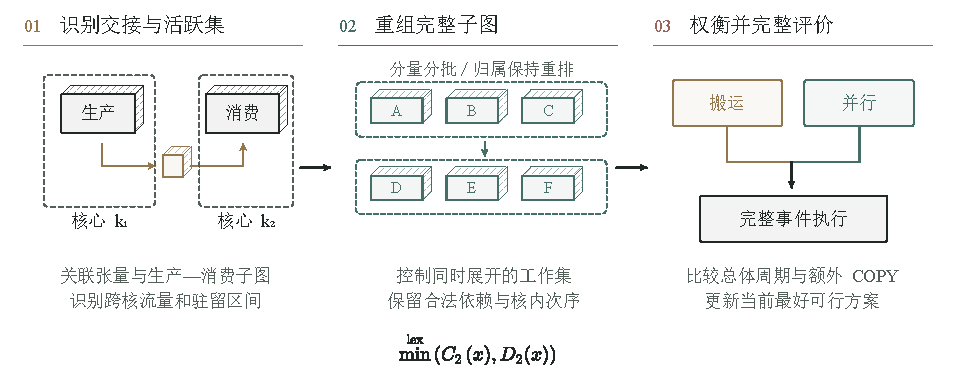
\includegraphics[width=\textwidth]{../求解/问题二/图片/q2_overview.pdf}
\caption{问题二的联合建模与迭代改进框架}\label{fig:q2_overview}
\end{figure}


\subsection{核心级任务的执行模型}
\subsubsection{同核驻留与跨核交接}
对核心 $k$，令 $\pi_k=(i_1,\ldots,i_{m_k})$，其全部子图属于同一 Task，任务标识为 $k$。同核相邻子图按方案顺序执行，但任务边界不在两者之间重复建立。若张量 $t$ 的生产者和后续消费者均位于 $k$，且执行过程未将相应缓冲换出，则消费者可读取本核驻留实例。图~\ref{fig:q2_task} 表示两类路径：同核复用沿着驻留状态传播，跨核依赖则先完成输出搬运，再进入目标核的读入队列。
\begin{figure}[htbp]\centering
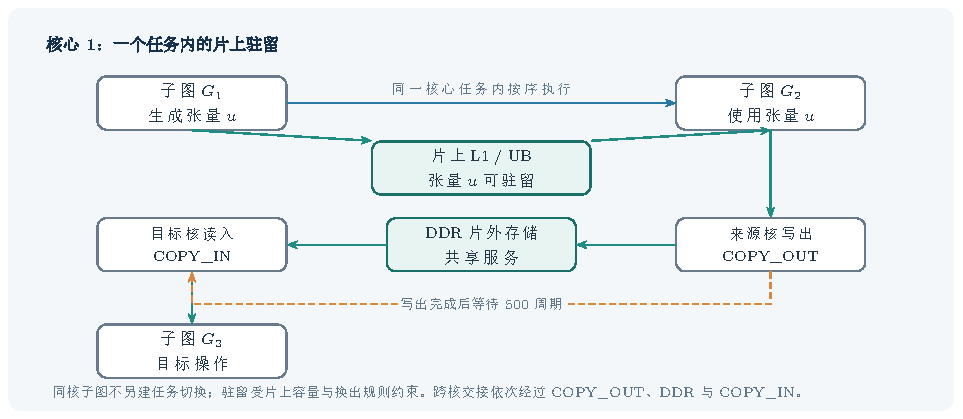
\includegraphics[width=\textwidth]{../求解/问题二/图片/q2_task.pdf}
\caption{核心级 Task 中的驻留与跨核交接}\label{fig:q2_task}
\end{figure}

对于跨核张量 $t$ 的一条交接，设相应 $\mathrm{COPY\_OUT}$ 完成于 $f_t^{\mathrm{out}}$，目标核的 $\mathrm{COPY\_IN}$ 开始于 $s_t^{\mathrm{in}}$。题设要求
\begin{equation}
 s_t^{\mathrm{in}}\ge f_t^{\mathrm{out}}+500.
 \label{eq:q2_handoff}
\end{equation}
若目标操作依赖多个跨核输入，则各输入分别满足式~\eqref{eq:q2_handoff}，其可启动时刻受最晚到达者约束。同核路径直接延续本核任务的存储状态。式~\eqref{eq:q2_handoff} 只是释放读入的必要条件：$\mathrm{COPY\_OUT}$ 和 $\mathrm{COPY\_IN}$ 本身占用共享 DDR，目标核读入流水线、缓冲容量及其他依赖还可能继续推迟完成时刻。

本问保持联合决策变量不变，采用核心级任务的执行映射 $\mathcal E_2$，优化问题为
\begin{equation}
 \min_{x\in\mathcal F_2}^{\mathrm{lex}}\bigl(C_2(x),D_2(x)\bigr).
 \label{eq:q2_problem}
\end{equation}
这里 $\mathcal F_2$ 仍由无环、容量和完整执行可行性共同确定。两问分别重建 COPY、缓冲生命周期和任务就绪时间，再由全局事件执行得到周期。

\subsubsection{活跃集、自动换出与共享带宽}
同核跨子图驻留扩大了复用机会，也延长了活跃区间。实际占用按式~\eqref{eq:capacity} 的缓冲实例集合 $\mathcal B_{k,r}(\tau)$ 检查。部分候选在来源内排序时采用换出前存储需求估计：将核心 $k$ 的子图按 $\pi_k$ 连接，组内按原图拓扑位置排列，得到算子序列。对序列中的张量，其估计生命期从首次生产位置开始；没有本核生产者时从首次使用位置开始，并延续至最后生产或使用位置。记位置 $h$ 上仍处于这一闭区间、归入存储区 $r$ 的张量集合为 $\widehat{\mathcal L}_{k,r}(h;x)$。原位置为DDR的张量在代理中按UB计，同一张量在各核分别计量。定义峰值估计
\begin{equation}
 \widehat M_r(x)=\max_{k,h}\sum_{t\in\widehat{\mathcal L}_{k,r}(h;x)}b_t,
 \qquad r\in\{\mathrm{L1},\mathrm{UB}\}.
 \label{eq:q2_livepeak}
\end{equation}
式~\eqref{eq:q2_livepeak} 估计了自动换出前的逻辑活跃需求，可用于定位候选的驻留压力。完整执行随后依据固定顺序、下一次使用位置和换出资格插入Spill/Retrieve，并按实际缓冲实例检查容量。联合调度与张量置换研究揭示了驻留状态与片外访问的耦合\cite{A16}；内存感知调度研究则讨论了拓扑顺序对活跃集合和峰值存储的影响\cite{A17}。本文将这些分析用于子图划分、归核和核内顺序的候选设计。

额外 COPY 字节 $D_2(x)$ 汇总重建边界搬运及自动换出等题设规定的计量项。搬运字节与执行时间之间还受到事件时序影响。若多个核心同时提交 DDR 请求，第~\ref{sec:q1} 章式~\eqref{eq:bandwidth} 的共享服务率取决于当时在途请求数。局部减少字节，可能因为请求从非关键段移至关键段而并未缩短总体任务执行时间；反过来，适度增加搬运，也可能提前释放依赖或让计算与通信重叠。因此，跨核 COPY 数、驻留峰值和计算负载在候选阶段用于解释与排序，最终保留仍由完整执行的 $(C_2,D_2)$ 判定。

\subsection{面向驻留与交接的候选改进}
\subsubsection{结构调整与关联子图迁移}
第二问的基础与结构候选沿用第一问的完整方案表达，包括不同粒度的初始划分，以及围绕当前可行方案的迁移、交换、拆分与联合迁移。由第~\ref{sec:q1} 章的全局下界 $L$ 可报告当前结果仍可能改进的范围；记当前可行周期为 $U$，当固定候选下界满足 $L(x)>U$ 时筛去该候选；等号情形保留，以比较额外COPY字节。核心级 Task 下，结构调整还有一项特殊价值：把生产者及消费它的子图放在同一核心，可能使跨核交接转为本核驻留读取。但共同归核会占用同一核心的计算 Pipe，并延长相应张量的生命期，其收益由完整执行评价确定。

对跨核使用频繁且字节数较大的张量，驻留来源先识别生产者和消费者涉及的完整子图集合，再取依赖与原有核序中需要一并移动的闭合子集，将这一组子图迁往某个已有归属核心。整体搬移保留原图依赖，并更新子图归核和相关核序。候选先检查无环性与核心顺序，再由完整评价检查容量并计算COPY和周期变化。多处理器调度中的局部迁移与多初值组织\cite{A42}为这种候选设计提供了一般思路。

另一个候选族保持原算子的核心归属，以依赖深度形成若干带，再按既有核心所有者划分子图。它试图把共享输入的使用收拢在较近的执行阶段，同时控制阶段内活跃集合；重新分组同时改变局部并行性与缓冲寿命。当图由相互独立的微小计算分量组成时，候选可把完整分量分配到核心，按容量估计限制每批同时展开的分量数，并将每批划成少量顺序阶段。分批宽度依据分量活跃峰值估计确定。两族候选分别面向连接较多和较分散的结构，实际容量按共同的完整评价流程检查。


\subsubsection{接受规则及质量解释}
所有来源都提交覆盖全部算子的完整 $x$，并在当前问题、核数及固定配置下接受执行检查。结构代理、活跃峰值和通信量只帮助产生候选，只有可行且 $(C_2,D_2)$ 字典序严格改善的结果才替换当前方案。第~\ref{sec:q1} 章命题3的归纳证明原样适用：已保留方案始终可行，目标序列单调不增。全局下界亦不因本问候选族改变而失效，因为其仅依赖保留的计算链、各类 Pipe 的总服务能力和已证明不可避的 DDR 流量。对五核结果，可计算 $1-L/C_2(x)$ 作为相对当前周期仍可能减少比例的上界。

\subsection{实验结果与机制分析}
\subsubsection{核数扩展与逐图周期}
按式~\eqref{eq:speedup} 对每图先求相对原始整图单核的加速比，再在 100 图上取算术平均。表~\ref{tab:q2_mean} 与图~\ref{fig:q2_mean} 给出第二问随核心数变化的结果。一至五核的平均加速比分别为 $1.0000$、$2.1168$、$3.0153$、$3.7868$ 和 $4.4538$；五核中位数为 $4.7143$。四核升至五核的平均增量仍为 $0.6670$，但低于二核升至三核的 $0.8985$。在核心级 Task 下，关键依赖链、各类计算 Pipe 的负载和共享 DDR 仍限制进一步并行。
% 由求解/规范化数据/combined/means.csv 生成；逐图加速比的算术平均。
\begin{table}[htbp]
\caption{问题二各核数逐图加速比统计}\label{tab:q2_mean}
\centering\normalsize
\setlength{\tabcolsep}{5pt}
\begin{tabular}{rrrrrr}
\toprule
核心数 & 样本数 & 平均加速比 & 中位加速比 & 最小加速比 & 最大加速比 \\
\midrule
1 & 100 & 1.0000 & 1.0000 & 1.0000 & 1.0000 \\
2 & 100 & 2.1168 & 2.0189 & 1.5706 & 3.6533 \\
3 & 100 & 3.0153 & 3.0064 & 1.7941 & 5.4726 \\
4 & 100 & 3.7868 & 3.9421 & 1.9552 & 7.0716 \\
5 & 100 & 4.4538 & 4.7143 & 1.9919 & 8.7768 \\
\bottomrule
\end{tabular}
\end{table}

\begin{figure}[htbp]\centering
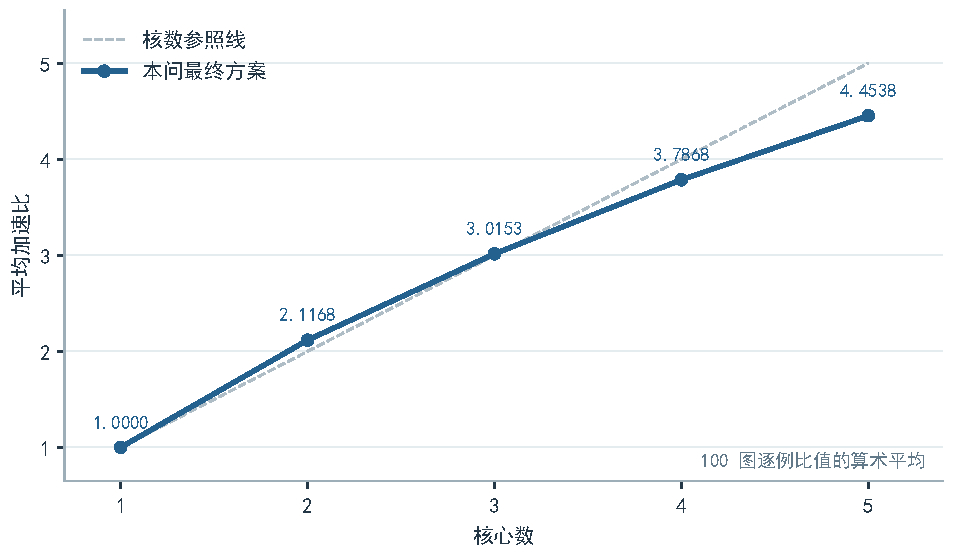
\includegraphics[width=.90\textwidth]{../求解/问题二/图片/q2_mean.pdf}
\caption{第二问各核数平均加速比}\label{fig:q2_mean}
\end{figure}

五核逐例加速比介于 $1.9919$ 和 $8.7768$，有 1 图低于 2，22 图高于 5。相对于原始整图单核参考，五核方案还调整了划分和核内顺序，搬运与自动换出也可能随之变化；因此这里的加速比可以超过五倍。五核周期的全局下界与当前结果所给相对差距上界，逐图平均为 $0.2462$；其中 6 图的界在 $1\%$ 以内。其余图的下界与可行周期之间仍有较宽区间。

图~\ref{fig:q2_distribution} 将同一批图的第一、二问五核加速比放在共同尺度上，并保留逐图点。第二问的分布整体向较高加速比移动，但仍有长尾与个别反例。为直接比较同一算例在两问中的执行周期，定义
\begin{equation}
 R_i=\frac{C_{i,1,5}}{C_{i,2,5}},\qquad i=1,\ldots,100.
 \label{eq:q2_pairratio}
\end{equation}
由于两问都以相同的 $T_{i,0}$ 定义加速比，$R_i$ 亦等于同图第二问加速比除以第一问加速比。100 图中 $R_i>1$ 有 89 图，$R_i=1$ 有 9 图，$R_i<1$ 有 2 图；比值均值 $1.1728$、中位数 $1.0913$。这组独立寻优结果表明，核心级 Task 下取得的最终方案在多数算例上更快。
\begin{figure}[htbp]\centering
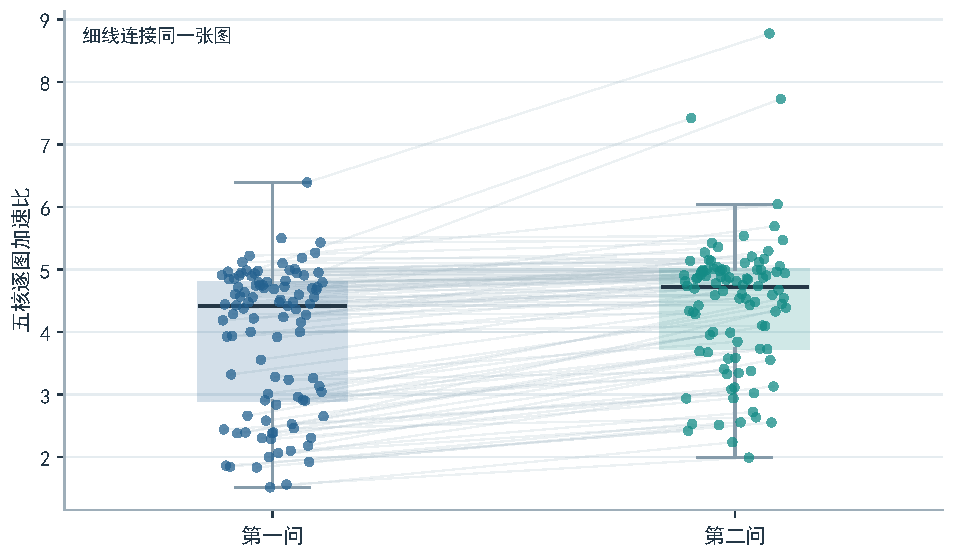
\includegraphics[width=.94\textwidth]{../求解/问题二/图片/q2_distribution.pdf}
\caption{五核逐图第一、二问加速比分布}\label{fig:q2_distribution}
\end{figure}

\subsubsection{COPY 量、驻留压力与反例}
第二问五核额外 COPY 字节的均值为 $8094619.10$ B，中位数为 $1310458$ B，均低于第一问的 $14585335.66$ B 和 $1990466$ B。逐图比较中，第二问有50个算例的额外COPY更少、12个相同、38个更多。图~\ref{fig:q2_copy} 按第二问减第一问的五核额外COPY字节差从小到大排列100个算例，依次分成四组，每组25个；纵轴为各问周期与本算例单核参考周期之比，每条线连接同一算例。COPY增加仍可能伴随周期缩短，因为方案可换取更早的跨核释放或更多计算重叠；COPY减少亦可能被更长的驻留区间和共享带宽争用抵消。
\begin{figure}[htbp]\centering
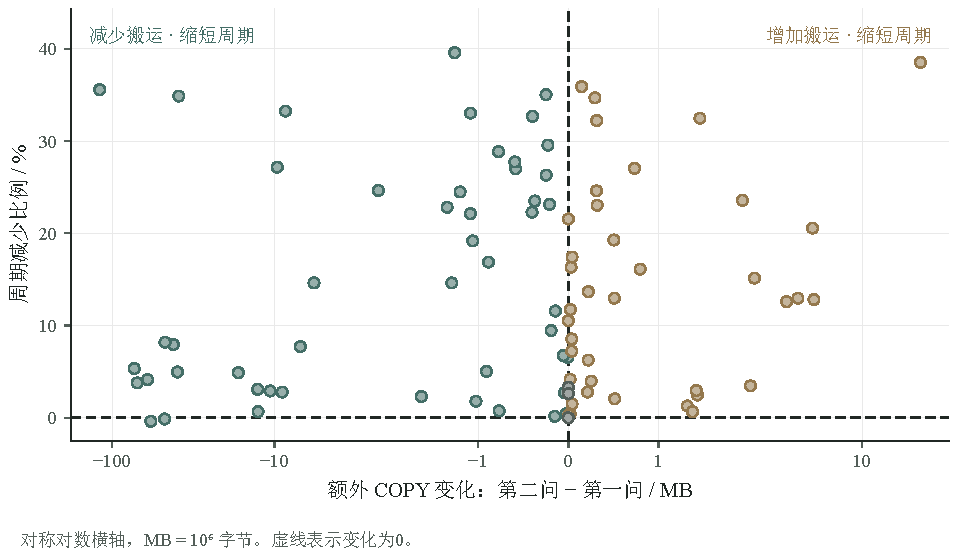
\includegraphics[width=.94\textwidth]{../求解/问题二/图片/q2_copy.pdf}
\caption{按COPY变化量分组的五核周期配对}\label{fig:q2_copy}
\end{figure}

边界搬运减少的同时，还需考察自动换出的变化。第一问五核有 88 图无自动换出，第二问为 74 图；第二问五核自动换出新增 COPY 字节的逐图均值为 $2645062.08$ B，高于第一问的 $206080.96$ B。同核驻留期延长可能增加容量压力，本组结果也记录到了更高的平均换出字节量。各算例的具体瓶颈仍需结合其执行轨迹定位。第二问周期略长的两个算例分别为算例072和算例079，其第一、二问五核周期为 $4775553/4781658$ 与 $5985137/6007992$；二者的第二问额外 COPY 字节反而都更少。这两个算例表明，额外COPY减少与周期缩短并不总是同步；关键路径、Pipe排队、活跃缓冲和DDR发射时机提供了进一步分析的方向。

\subsubsection{候选来源的调用与改善}
图~\ref{fig:q2_sources} 汇总第二问实际候选来源的调用和周期改善记录。结构来源完成评价 $15656$ 次，其中 $740$ 次带来周期改善；基础来源为 $8589$ 次及 $443$ 次，驻留来源为 $8819$ 次及 $353$ 次。三类来源均在联合搜索中取得过周期改善。它们相继更新同一个当前方案，调用机会随图结构、近期收益和剩余预算变化；这里统计的是联合运行表现，各来源的独立贡献有待控制来源的对照实验评估。
\begin{figure}[H]\centering
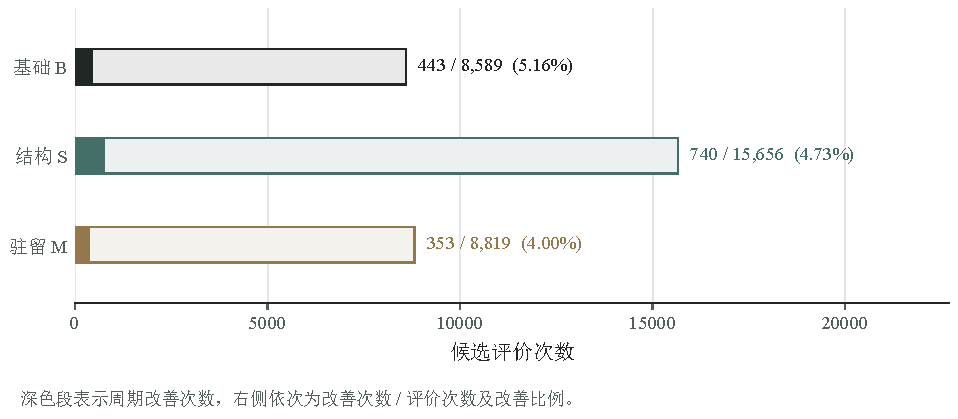
\includegraphics[width=.94\textwidth]{../求解/问题二/图片/q2_sources.pdf}
\caption{第二问候选来源的调用与周期改善记录}\label{fig:q2_sources}
\end{figure}

综合逐图周期、COPY 量和存储记录，第二问的主要机会来自同核跨子图复用与更细的跨核释放，但两者同时改变并行性和片上驻留压力。下一问在本问核心级 Task 基础上加入共享只读缓存，需进一步把逻辑 COPY 请求量与实际 DDR 服务量区分。

\GMCMChapterEnd{5}
\section{问题三求解与分析}
\label{sec:q3}
\subsection{问题的描述与分析}
第三问沿用第二问的核心级Task语义及划分、归核和核内顺序三个决策变量，并在各核的读入路径前加入容量为 $1048576$ B 的共享只读 L2。计算依赖与写出要求仍按原图执行，缓存为部分 $\mathrm{COPY\_IN}$ 提供新的服务路径。若读入命中，数据经 L2 带宽池服务；未命中时经DDR服务。每次读入完成时尝试填充，已驻留对象保持原队列位置。由此，哪一次请求能命中取决于全局读入发射、完成与淘汰的交错，并受张量复用关系影响。

图~\ref{fig:q3_overview} 展示本问的分析与求解流程：以第二问完整方案空间为基础，记录真实缓存事件，从观察到的重复未命中或淘汰窗口提出合法核内顺序候选，再用完整执行评价决定是否接受。实验分为三种口径：100 图的第三问主结果，同一第三问方案有无 L2 的配对结果，以及六张定向图在固定方案下的容量、带宽格点。三者分别刻画总体性能、固定方案缓存收益和定向参数响应。
\begin{figure}[htbp]
\centering
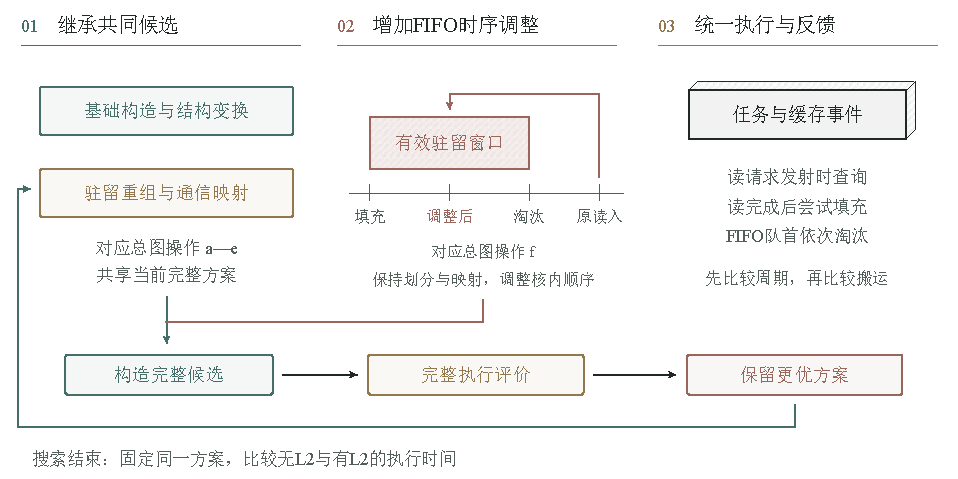
\includegraphics[width=\textwidth]{../求解/问题三/图片/q3_overview.pdf}
\caption{问题三的联合建模与迭代改进框架}\label{fig:q3_overview}
\end{figure}


\subsection{共享只读 L2 的事件模型}
\subsubsection{发射查询、完成填充与 FIFO 顺序}
记全局缓存状态 $\mathcal Q$ 为按成功填入先后排列的逻辑张量标识队列，$B_{\mathrm{L2}}$ 为缓存容量，队列占用按张量字节之和计。同周期事件按执行器次序逐项更新队列。对张量 $t$ 的一次读入请求 $r$，在实际发射时刻 $s_r$ 查询该发射事件之前的队列状态。若命中，则读入由 L2 池服务，并保持 $t$ 的队列位置；若未命中，则请求由 DDR 池服务。每次 $\mathrm{COPY\_IN}$ 在完成时刻 $f_r$ 触发填充尝试：若 $t$ 仍在队列中则保持原状态；若已不在队列且大小可容纳，则依次淘汰队首对象，为 $t$ 腾出空间后插入队尾。尺寸超过容量的张量跳过填充。因此，命中读若在服务期间经历淘汰，也会在完成时重新插入。图~\ref{fig:q3_fifo} 展示查询、路径选择与FIFO填充的处理流程。
\begin{figure}[htbp]\centering
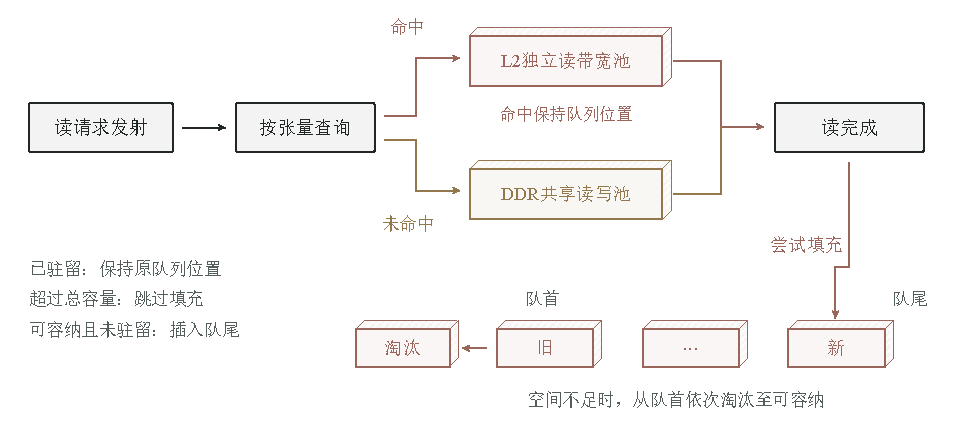
\includegraphics[width=.96\textwidth]{../求解/问题三/图片/q3_fifo.pdf}
\caption{FIFO 读入查询、完成填充与淘汰事件}\label{fig:q3_fifo}
\end{figure}

这一规则尤其影响并发读入。若两核在 $t$ 首次 DDR 读尚未完成时先后发射对 $t$ 的请求，二者查询时 $t\notin\mathcal Q$，因而可以同时未命中。另一方面，已命中的张量即使频繁被读取，也不会因命中刷新 FIFO 位置，后续插入仍可能将其淘汰。已有缓存感知DAG调度研究讨论了节点亲和性与延迟执行对复用的影响\cite{A40}。本题采用FIFO规则，命中由完成填充及后续淘汰形成的驻留区间决定。

第~\ref{subsec:q3_trace_analysis} 节以算例080的张量甲、乙对照这两类时序：甲的后续读取晚于淘汰，乙的一次读取位于驻留期内。缓存时序候选据此尝试调整完整子图的位置，使后续读取有机会落入有效驻留窗口。

\subsubsection{两个共享服务池与计量口径}
设时刻 $\tau$ 在途DDR读写请求集合为 $\mathcal A_D(\tau)$，包括未命中读与写出；在途L2命中读请求集合为 $\mathcal A_L(\tau)$。两池分别以 $60$ B/周期和 $250$ B/周期的总带宽服务，并按各自在途请求数共享；在事件集合不变的区间，某请求以独占服务周期表示的剩余量满足
\begin{equation}
 w_j(\tau+\Delta)=
 \max\!\left\{0,w_j(\tau)-\frac{\Delta}{|\mathcal A_h(\tau)|}\right\},
 \quad j\in\mathcal A_h(\tau),\quad h\in\{D,L\}.
 \label{eq:q3_two_pools}
\end{equation}
两种 $w_j$ 分别按请求所属服务池的带宽换算。DDR 写出和未命中读仍与其他 DDR 请求争用；命中读虽不经 DDR，仍占 L2 池及对应读入流水线，并可能受前驱、缓冲容量和核心内部顺序约束。命中降低该次读的DDR服务需求，其总体收益还取决于请求是否影响关键完成路径。

设 $B_i^{\rm hit}$ 与 $B_i^{\rm miss}$ 为某执行中 \texttt{COPY\_IN} 经 L2 命中和未命中的字节，定义按字节计的命中率
\begin{equation}
 H_i=\frac{B_i^{\rm hit}}{B_i^{\rm hit}+B_i^{\rm miss}}.
 \label{eq:q3_hit}
\end{equation}
当分母非零时，$H_i$ 描述命中字节占全部读入字节的比例。$D_3(x)$ 则按第~\ref{sec:q1} 章的额外COPY口径统计，包括相关的逻辑读入操作。两项指标分别反映服务路径与搬运规模。最终周期还由计算关键链、写出、两池并发以及填充造成的 FIFO 变化共同决定。

\subsection{缓存时序候选与统一接受规则}
\subsubsection{合法顺序邻域}
第三问沿用基础、结构和驻留候选，并增设由已评价缓存轨迹驱动的顺序候选。设当前方案为 $x=(\mathcal P,a,\boldsymbol\pi)$，此来源产生的 $x'=(\mathcal P,a,\boldsymbol\pi')$ 保持算子到子图的划分及子图到核心的归属，只在一个或两个核心的 $\pi_k$ 中移动完整子图。于是原始算子覆盖、每个算子的核心归属与跨核边集合保持不变；但局部先后、读入发射时刻、Spill、FIFO 队列和完成时刻都可能变化。候选随后检查核序与跨核依赖合图的无环性，再作完整执行评价。

从实际未命中记录中，可辨别读入发射时尚有相同张量的在途填充、或上一次缓存副本已被淘汰两类窗口。第一类候选试着将消费者子图后移，或把产生首次有效填充的读者子图前移，让后续发射有机会落在填充之后。第二类候选试着把消费者前移，或把引发实际淘汰的填入者后移，让复用落在淘汰之前。还可联合不同核心上的两次局部移动，并按相邻子图的计算工作量估计需要跨过的时间窗口。移动距离依据原轨迹估计；调整后重新生成所有请求的交错并计算实际命中。候选在来源内去重，经过结构检查、下界筛选和完整执行，才按 $(C_3,D_3)$ 的字典序与当前方案比较。

上述填充与淘汰机制说明，FIFO顺序由成功填入事件决定。静态相邻的消费者仍可能在不同的驻留区间发射请求。来源选择沿用第~\ref{sec:q1} 章的近期收益、运行成本和访问间隔规则，按测量反馈分配有限的搜索机会\cite{A12}。所有来源共享同一当前可行方案，结构或驻留候选被接受后，缓存事件候选会围绕新的执行轨迹重新提出。

\subsubsection{同方案配对的识别量}
令 $x_{i,3,n}$ 为图 $i$、$n$ 核下第三问选出的完整方案。将\emph{同一个方案}分别置于有 L2 和无 L2 的执行环境，定义
\begin{equation}
 R^{\rm L2}_{i,n}=
 \frac{C_2(x_{i,3,n})}{C_3(x_{i,3,n})}.
 \label{eq:q3_pair}
\end{equation}
两次执行保持 $\mathcal P,a,\boldsymbol\pi$ 一致，仅改变缓存规则。式~\eqref{eq:q3_pair} 衡量第三问所选方案的缓存影响；两问各自寻优后的比较则使用各自选出的方案，回答不同的性能问题。

\subsection{主实验与定向参数研究}
\subsubsection{核数扩展、独立优化与同方案对照}
第三问仍用式~\eqref{eq:speedup} 的逐图算术平均。表~\ref{tab:q3_mean} 与图~\ref{fig:q3_mean} 给出一至五核主结果，平均加速比分别为 $1.1008$、$2.1222$、$3.0320$、$3.8376$、$4.5978$，五核中位数为 $4.8565$。一核结果可以高于 1，因为原始单核参考没有按第三问的方案和缓存条件重新优化；多核结果也包含重新分组与顺序的影响。图中的无L2参考曲线也以 $T_{i,0}$ 为分子：对相同第三问方案，逐图计算 $T_{i,0}/C_2(x_{i,3,n})$，再取100图的算术平均。它与有L2曲线使用同一单核基准；固定方案的缓存周期比另由式~\eqref{eq:q3_pair} 给出。
% 由求解/规范化数据/combined/means.csv 生成；逐图加速比的算术平均。
\begin{table}[htbp]
\caption{问题三各核数逐图加速比统计}\label{tab:q3_mean}
\centering\normalsize
\setlength{\tabcolsep}{5pt}
\begin{tabular}{rrrrrr}
\toprule
核心数 & 样本数 & 平均加速比 & 中位加速比 & 最小加速比 & 最大加速比 \\
\midrule
1 & 100 & 1.1008 & 1.0427 & 0.9969 & 2.0540 \\
2 & 100 & 2.1222 & 2.0271 & 1.5225 & 3.6533 \\
3 & 100 & 3.0320 & 3.0182 & 1.7667 & 5.4726 \\
4 & 100 & 3.8376 & 3.9656 & 1.9853 & 7.0949 \\
5 & 100 & 4.5978 & 4.8565 & 2.0717 & 8.7768 \\
\bottomrule
\end{tabular}
\end{table}

\begin{figure}[htbp]\centering
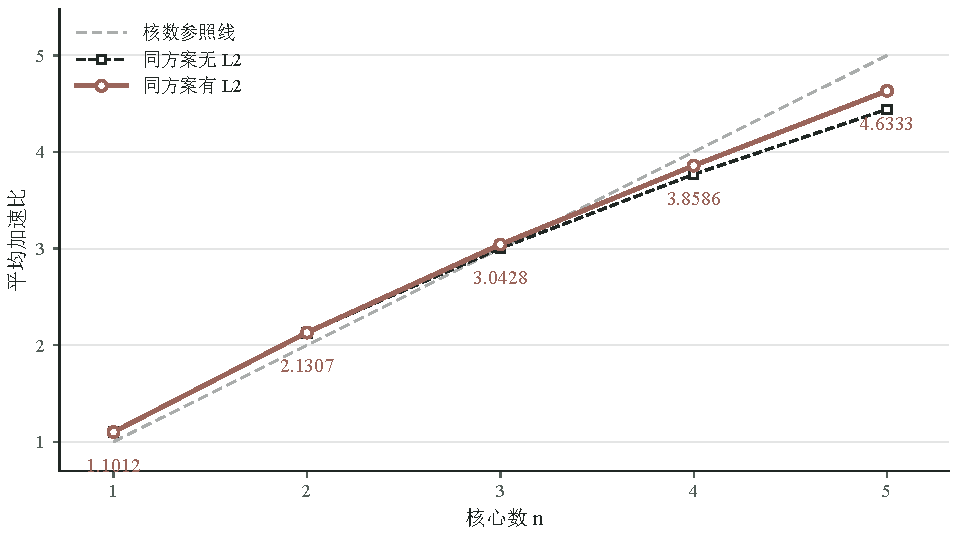
\includegraphics[width=.91\textwidth]{../求解/问题三/图片/q3_mean.pdf}
\caption{第三问各核数主结果及同方案无 L2 参考}\label{fig:q3_mean}
\end{figure}

若改用两问各自选出的五核方案相较，第三问在 100 图中有 66 图周期短于第二问、18 图相等、16 图更长。该对照同时包含两问的执行规则与方案选择差异。第三问五核额外 COPY 字节均值为 $8293721.4$ B，中位数为 $1484117$ B；它们与第二问使用相同的逻辑搬运统计口径。逻辑COPY和自动换出量可能随所选方案变化，读入请求的服务路径则随缓存命中情况变化。

同方案配对覆盖 100 图的全部五种核数，共 500 组。各核数样本量、平均和中位周期比列于表~\ref{tab:q3_pairs}，经验分布见图~\ref{fig:q3_pairs}。五核平均周期比为 $1.0558$，中位数为 $1.0077$；77 图的周期缩短，23 图相等。周期比集中在1附近，说明许多方案的总体完成周期变化较小；右侧尾部对应缓存收益较大的少数算例。
% PR60–62：90组新配对、410组同方案继承；均值是逐例比值的算术平均。
\begin{table}[htbp]
\caption{第三问同一方案有无 L2 的周期配对统计}\label{tab:q3_pairs}
\centering\normalsize
\setlength{\tabcolsep}{4pt}
\begin{tabular}{rrrrrrrr}
\toprule
核数 & 配对数 & \shortstack{平均\\周期比} & \shortstack{中位\\周期比} & 改善 & 相同 & 退化 & \shortstack{平均字节\\命中率} \\
\midrule
1 & 100 & 1.0003 & 1.0000 & 28 & 72 & 0 & 0.0586 \\
2 & 100 & 1.0013 & 1.0001 & 55 & 45 & 0 & 0.1494 \\
3 & 100 & 1.0145 & 1.0004 & 61 & 39 & 0 & 0.2245 \\
4 & 100 & 1.0290 & 1.0019 & 72 & 28 & 0 & 0.2449 \\
5 & 100 & 1.0560 & 1.0082 & 76 & 24 & 0 & 0.3004 \\
\bottomrule
\end{tabular}
\end{table}

\begin{figure}[htbp]\centering
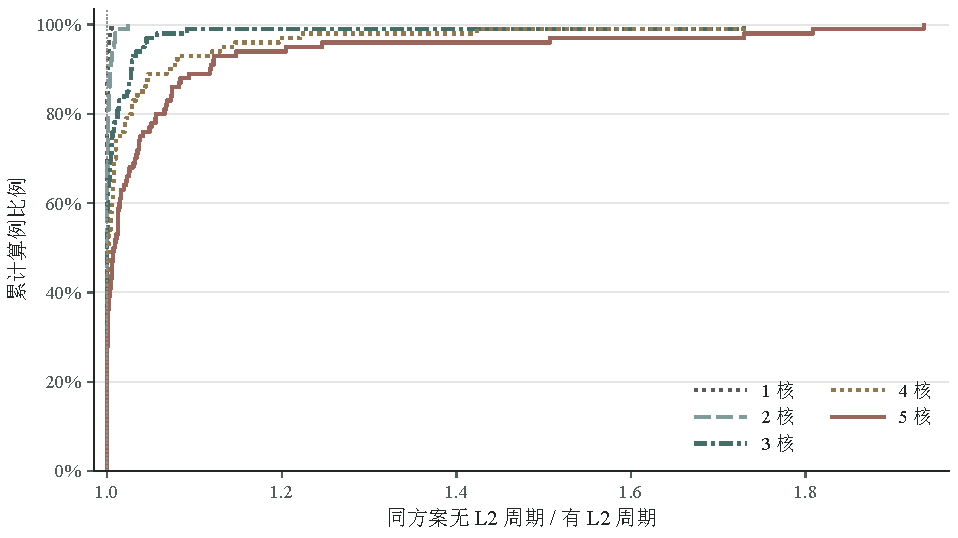
\includegraphics[width=.92\textwidth]{../求解/问题三/图片/q3_pairs.pdf}
\caption{各核数同方案缓存周期比的经验分布}\label{fig:q3_pairs}
\end{figure}

图~\ref{fig:q3_hit_gain} 对照逐例命中字节率与式~\eqref{eq:q3_pair}。解释逐例收益时，需要同时考虑命中位置与事件时序：命中若落在非关键请求上，可能不改变总体任务执行时间；低命中率也可能恰好覆盖关键链上的少量大请求。散点展示了命中率相近的方案仍可能具有不同周期收益的现象。第三问主结果的全局下界与当前五核周期给出的相对差距上界逐图平均为 $0.2248$；其中 6 图在 $1\%$ 以内。该界由计算路径、Pipe负载和对全部可行方案成立的必要流量松弛得到。
\begin{figure}[htbp]\centering
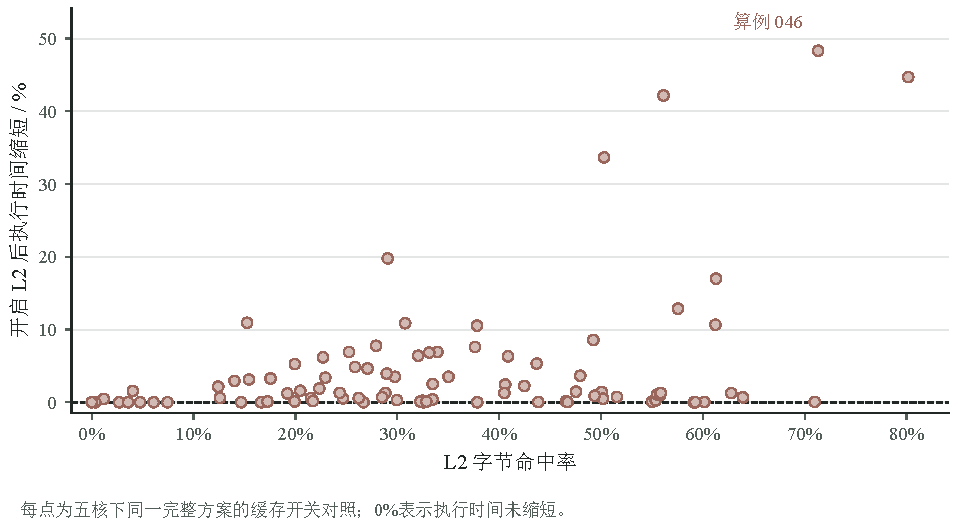
\includegraphics[width=.92\textwidth]{../求解/问题三/图片/q3_hit_gain.pdf}
\caption{字节命中率与同方案缓存周期比}\label{fig:q3_hit_gain}
\end{figure}

\subsubsection{固定方案的容量—带宽响应面}
为观察参数敏感性，从主实验中定向选取六张图，每图固定一份五核完整方案，分别在 L2 容量 $262144$、$1048576$、$4194304$ B，与 L2 带宽 $60$、$250$、$500$ B/周期的九个组合下执行。图~\ref{fig:q3_parameters} 展示共 54 个固定方案格点的真实周期；其中各图的默认配置格沿用对应主实验响应。由于一张图的九格使用同一划分、归核和顺序，格内差异反映该固定方案对参数变化的响应。六个定向算例用于展示不同的缓存机制与敏感性。
\begin{figure}[htbp]\centering
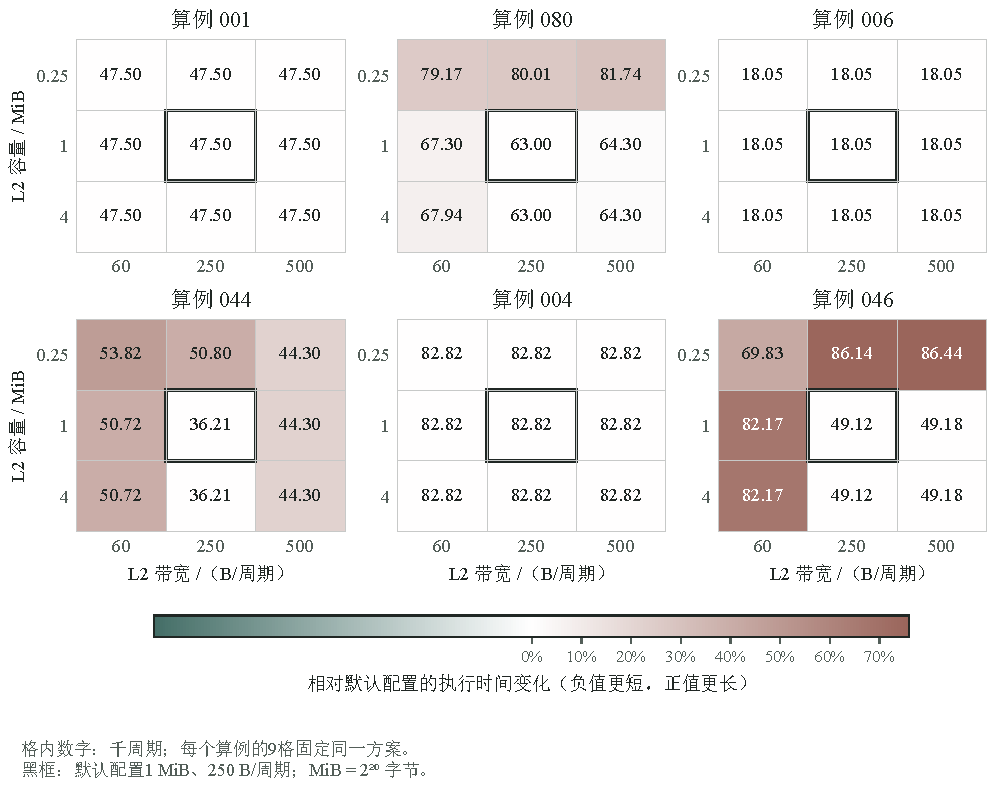
\includegraphics[width=.96\textwidth]{../求解/问题三/图片/q3_parameters.pdf}
\caption{六图固定方案的 L2 容量与带宽周期响应}\label{fig:q3_parameters}
\end{figure}

算例080在带宽固定为 $250$ B/周期时，容量从 $262144$ B 增至 $1048576$ B，周期从 $80014$ 降至 $63001$，字节命中率从 $0.1827$ 升至 $0.5031$。算例001的九个格点均为 $47502$ 周期且零命中，表明提高缓存容量或 L2 带宽只有在相应读入真正利用缓存并影响完成路径时才可能奏效。另在每图的两个边界参数配置下重新适配方案，共取得12个观察值，用于观察参数改变后的重新优化表现；其配置与结果列于支撑材料。

由事件、配对与参数格可见，缓存时序优化需要使关键请求落在有效FIFO驻留窗口内，同时协调L2池与读入Pipe的争用。下面结合具体张量的填充与淘汰事件，分析这些参数响应中的时序差异。

\subsection{缓存驻留窗口的推导与逐事件分析}
\subsubsection{先进先出驻留窗口}
缓存时序候选需要判断一次顺序移动试图跨过哪个事件。考察张量 $t$ 成功填入后、首次淘汰前的一段驻留期，设其大小为 $b_t\le B_{\mathrm{L2}}$。按评估程序的事件次序编号，$e_f$ 表示本次填充事件，$A_t(e)$ 表示从 $e_f$ 之后到事件 $e$ 新插入队尾的对象字节总和。已驻留对象的查询或再次填充不计入，超容量而未入队的对象也不计入。

\textbf{命题4：}若填入只在容量不足时按FIFO顺序淘汰、命中不刷新队列位置，且不发生其他删除，则 $t$ 的首次淘汰事件为：
\begin{equation}
 e_v=\min\{e>e_f:e\text{ 为新填入事件，且 }b_t+A_t(e)>B_{\mathrm{L2}}\}.
 \label{eq:q3_fifo_eviction}
\end{equation}

若集合为空，则本段驻留期内不发生淘汰。

\textbf{证明：}在首次淘汰前，原有对象排在 $t$ 前，新填入对象排在 $t$ 后。设新填入事件 $e$ 之前，$t$ 前方对象的总字节数为 $O_e$，后方为 $A_t(e^-)$，本次插入对象大小为 $b_e\le B_{\mathrm{L2}}$。由于FIFO不会先淘汰 $t$ 后方的对象，有 $A_t(e)=A_t(e^-)+b_e$。此次至少需释放的字节数为：
\[
 R_e=\max\{0,O_e+b_t+A_t(e)-B_{\mathrm{L2}}\}.
\]

前方对象能提供的空间为 $O_e$，故：
\[
 \begin{aligned}
 R_e\le O_e&\ \Longleftrightarrow\ b_t+A_t(e)\le B_{\mathrm{L2}},\\
 R_e>O_e&\ \Longleftrightarrow\ b_t+A_t(e)>B_{\mathrm{L2}}.
 \end{aligned}
\]

第一种情形在移除部分旧前缀后即可填入，$t$ 保留。第二种情形移除全部旧前缀仍不够，队首的 $t$ 随即被淘汰。取第二种情形首次成立的事件即得式~\eqref{eq:q3_fifo_eviction}。

令 $e_r$ 为向使用算子供给该张量的读入请求的发射事件，$\prec$ 表示评估程序中的先后次序。该次读入命中这段驻留期的条件为：
\begin{equation}
 e_f\prec e_r\prec e_v.
 \label{eq:cachewindow}
\end{equation}

若尚未淘汰，把右端点视为无穷远。三个事件的周期分别记为 $f_t,s_t,e_t$。仅在时刻互异时，式~\eqref{eq:cachewindow} 才可简写为 $f_t<s_t<e_t$。同周期的填充、淘汰与查询仍按实际事件次序判断。

式~\eqref{eq:cachewindow} 是固定事件序列的性质。移动子图会改变计算完成、请求发射与带宽共享，进而同时改变 $f_t$、$e_t$ 和 $s_t$。实际方法据原轨迹提出移动方向，再重建整个执行过程。新方案中的驻留窗口随新轨迹重新确定。

\subsubsection{算例080的填充、命中与淘汰}
\label{subsec:q3_trace_analysis}
取参数研究中算例080的五核固定方案，L2 容量为 $262144$ B，带宽为 $60$ B/周期。图~\ref{fig:q3_trace} 上部展示张量甲（4096 B）与张量乙（8192 B）的驻留区间及访问事件，下部放大前1400周期的五核读入轨迹。色带末端箭头表示驻留延续至观察窗以外。
\begin{figure}[htbp]\centering
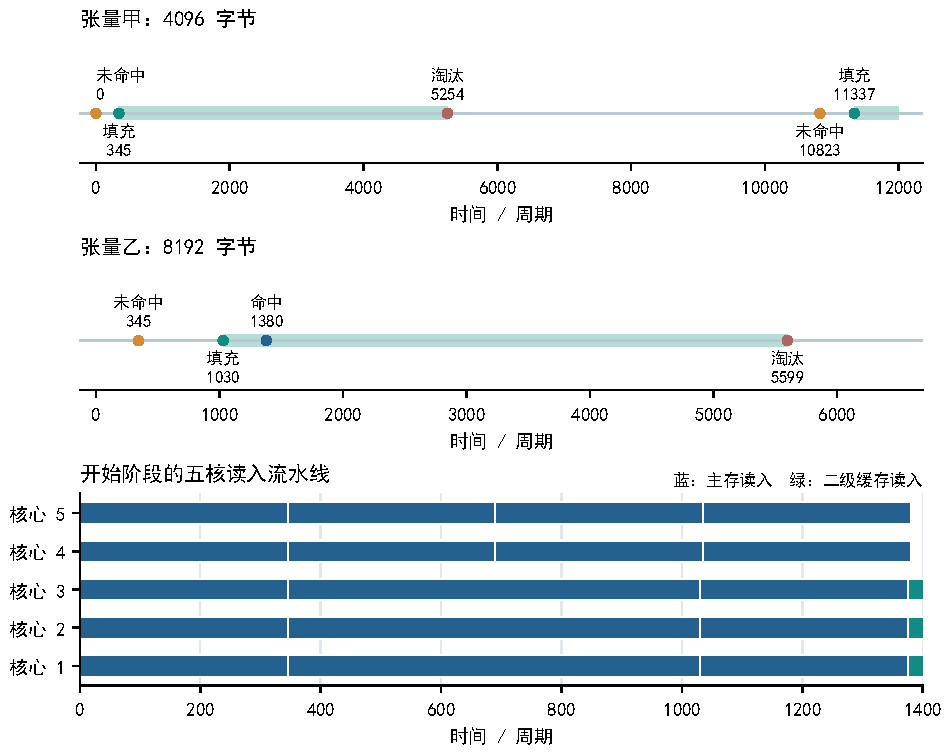
\includegraphics[width=\textwidth]{../求解/问题三/图片/q3_trace.pdf}
\caption{算例080的缓存驻留窗口与多核读入轨迹}\label{fig:q3_trace}
\end{figure}

张量甲在周期0的读取未命中，读入于周期345完成后进入缓存。周期5254的一次新填入将它淘汰。当另一核心在周期10823再次读入甲时，访问已落在这段驻留窗口之外，因此再次未命中。甲在周期11337重新填入，于周期15878再次被淘汰。周期21536的下一次读取仍未命中。

张量乙在周期345查询时未命中，于周期1030填充。周期1380的查询发生在其驻留期内，因而命中。此命中没有将乙移至队尾，周期5599它仍被后续填入淘汰。

图中最早的五个读请求均在周期0发射、周期345完成，显示共享 DDR 上的并发服务。对甲的 $4096$ B 请求，按每请求独占服务周期向上取整得到 $\lceil4096/60\rceil=69$ 周期。在这五个请求同时在途的区间，共享服务使其完成周期与 $5\times69=345$ 一致。

\subsubsection{固定方案的容量与带宽响应}
图~\ref{fig:q3_parameters} 的54个格点保持每张图的五核完整方案不变。算例080在容量 $262144$ B 下，L2 带宽依次为 $60$、$250$、$500$ B/周期时，总体任务执行时间依次为 $79170$、$80014$、$81744$ 周期。对应字节命中率为 $0.1960$、$0.1827$、$0.1680$。带宽提高后，命中率下降而总体任务执行时间上升，表明服务速度的改变伴随缓存访问状态变化。按照前述事件模型，服务完成时刻会影响后续请求发射、缓存填充与淘汰的相对次序。

容量响应也出现平台：算例080在带宽 $250$ B/周期下，容量从 $262144$ B 增至 $1048576$ B 时，周期由 $80014$ 降为 $63001$。继续增至 $4194304$ B，周期仍为 $63001$。算例044在容量 $1048576$ B 下，带宽从 $60$ 增至 $250$、$500$ B/周期，周期为 $50723$、$36208$、$44299$。这两组固定方案结果分别展示了容量增加后的平台和带宽增加后的周期回升，说明需要在完整事件执行中联合评价容量与带宽配置。

算例046五核同方案有L2和无L2的周期分别为 $49119$ 与 $95050$，周期比为 $1.9351$，字节命中率约为 $0.7132$。


\GMCMChapterEnd{6}
\section{模型评价与展望}
\subsection{模型优点}
\begin{enumerate}
\item 三问使用同一完整方案 $x=(\mathcal P,a,\boldsymbol\pi)$ 与字典序目标。子图划分、核心映射和核内顺序通过各问的执行映射共同作用于总体任务执行时间。第一问的子图级 Task、第二问的核心级 Task 以及第三问的 FIFO 缓存，都能在统一方案空间内比较。

\item 目标值由完整事件执行确定。片上 L1/UB 按缓冲实例检查瞬时容量，自动换出按固定规则插入。矩阵、向量及读写流水线各受占用约束，DDR 与 L2 带宽按在途请求共享。通信量和活跃峰值用于候选排序，下界用于筛选，完整事件执行确定最终周期。第三问的同方案配对固定子图划分、核心映射和核内顺序，使缓存对照具有明确的比较对象。

\item 多种候选来源共同改进一个已经验证的可行方案。结构移动提供并行度调整，驻留候选响应张量生命周期和跨核通信，缓存时序候选定位真实的未命中、填充与淘汰窗口。每次只接受完整评价可行且目标字典序改善的方案，保证已保留结果的可行性和单调性。全局下界给出相对当前周期仍可能降低的有效上界，可用于判定近界停止，并量化停止时的质量范围。
\end{enumerate}

\subsection{模型缺点}
\begin{enumerate}
\item 完整评价成本较高。通过结构预检、去重和下界筛选而进入完整评价的候选，需要重建任务、COPY、换入换出和全局事件序列。在共享带宽与 FIFO 状态耦合较强的图上，细小的顺序移动也可能引发大量事件变化。图规模、请求密度和评价成本因而限制可考察的候选数量。

\item 存储与带宽估计对事件时序的表达有限。按逻辑活跃集估计的峰值不能精确替代按缓冲实例计量的 L1/UB 占用。静态跨核字节也不包含读写请求的同时在途程度。第三问的读取可能发生在填充前或淘汰后，静态估计因而可能错排候选。

\item 来源调用记录中的改善次数受调用顺序和当前方案影响，难以单独量化各邻域的贡献。后续可固定初始方案与预算，逐项关闭邻域进行对照。六图容量与带宽研究也可扩展到全部算例，以考察参数响应的普遍性。
\end{enumerate}

\subsection{模型的推广与改进}
可进一步发展针对事件耦合的增量评价。候选只移动少量完整子图时，先确定受影响的依赖后继、同核 Pipe 队列和张量生命周期，再从最早变化事件向后更新。若能证明未波及部分的状态和就绪时刻不变，即可避免每次从头执行全图。增量结果仍应与完整事件语义等价，并在状态变化越过核心或带宽池时扩大重算范围。结合更紧的候选下界，可用节省的时间考察更多候选。

对缓存问题，可把轨迹中的读入发射、完成填充和淘汰构成显式窗口图，估计候选移动对关键请求所在窗口的影响。估计应同时考虑两带宽池、读入流水线和关键链。推广到允许选择缓存替换、预取或张量重算策略的场景时，可在现有 $x$ 之外增加相应决策变量，并重新证明可行性与下界。

\GMCMChapterEnd{7}
\clearpage
\nocite{ai_tool_disclosure}
\bibliographystyle{gmcm}
\bibliography{references}

\GMCMChapterEnd{8}
\clearpage
% Generated by tools/build_appendix.py; do not hand-edit.
% Styling is owned exclusively by 章节模板/附录模板.tex.
\AppendixStart
\AppendixPart{1}{附件文件及内容}
\AppendixAttachmentTableBegin
\AppendixAttachmentRow{1}{问题一}{完整方法源码、代码环境说明和 Task/调度逐例结果表。}
\AppendixAttachmentRow{2}{问题二}{完整方法源码、代码环境说明和跨核交接/DDR 逐例结果表。}
\AppendixAttachmentRow{3}{问题三}{完整方法源码、代码环境说明和 L2/FIFO 同方案配对逐例结果表。}
\AppendixAttachmentRow{4}{其他数据}{100 个原始计算图、官方配置、完整官方评价代码及来源说明。}
\AppendixAttachmentRow{5}{其他支撑材料}{1400 个已选主配置和 500 个同方案配对的计划/官方响应、各分片执行源码、数据表及整理复现程序。}
\AppendixAttachmentTableEnd
\AppendixPart{2}{问题一关键代码}
\AppendixCodeFile[firstline=58,lastline=121,firstnumber=58]{官方评价与字典序接受（片段 1）}{python}{../提交附件/支撑材料文件/问题一/源码/research_a_orion_trident/solve.py}
\AppendixCodeFile[firstline=43,lastline=49,firstnumber=43]{初始结构候选构造（片段 2）}{python}{../提交附件/支撑材料文件/问题一/源码/research_a_orion_trident/sources.py}
\AppendixPart{3}{问题二关键代码}
\AppendixCodeFile[firstline=350,lastline=376,firstnumber=350]{跨核交接与 DDR 搬运量（片段 1）}{python}{../提交附件/支撑材料文件/问题二/源码/research_a_orion_trident/vendor/orion/core.py}
\AppendixCodeFile[firstline=377,lastline=431,firstnumber=377]{全局及候选下界（片段 2）}{python}{../提交附件/支撑材料文件/问题二/源码/research_a_orion_trident/vendor/orion/core.py}
\AppendixPart{4}{问题三关键代码}
\AppendixCodeFile[firstline=19,lastline=63,firstnumber=19]{FIFO 事件驱动的候选定位与顺序移动（片段 1）}{python}{../提交附件/支撑材料文件/问题三/源码/research_a_orion_trident/fifo.py}
\AppendixCodeFile[firstline=258,lastline=275,firstnumber=258]{同一完整方案的无 L2 官方配对（片段 2）}{python}{../提交附件/支撑材料文件/问题三/源码/research_a_orion_trident/solve.py}
\AppendixPart{5}{逐例结果与同方案配对}
% 可选附录长表；每表最多两个核数，表宽不超过 160 mm。

% 问题一、二的 1 核行从规范化 appendix_q1/q2.csv 中题设单核约定读取，不由多核公式回填。

% 周期为总体任务执行时间；字节为额外 COPY。q1/q2 单核使用题设约定的原始整图响应。
\begingroup\normalsize
\setlength{\tabcolsep}{3pt}
\setlength{\LTleft}{\fill}\setlength{\LTright}{\fill}
\setlength{\LTcapwidth}{160mm}
\begin{longtable}{@{}p{15mm}>{\raggedleft\arraybackslash}p{28mm}>{\raggedleft\arraybackslash}p{39mm}>{\raggedleft\arraybackslash}p{28mm}>{\raggedleft\arraybackslash}p{39mm}@{}}
\caption{问题一逐例结果：1、2 核}\label{tab:appendix_q1_n12}\\
\toprule
算例 & \shortstack{1 核\\周期} & \shortstack{1 核额外\\COPY/B} & \shortstack{2 核\\周期} & \shortstack{2 核额外\\COPY/B}\\
\midrule
\endfirsthead
\caption[]{问题一逐例结果：1、2 核（续）}\\
\toprule
算例 & \shortstack{1 核\\周期} & \shortstack{1 核额外\\COPY/B} & \shortstack{2 核\\周期} & \shortstack{2 核额外\\COPY/B}\\
\midrule
\endhead
\bottomrule
\endfoot
001 & 233,110 & 0 & 116,868 & 1,152\\
002 & 261,945 & 0 & 130,549 & 1,585,152\\
003 & 602,212 & 0 & 356,773 & 5,569,332\\
004 & 392,357 & 0 & 199,074 & 110,592\\
005 & 95,618 & 0 & 62,870 & 1,034,798\\
006 & 82,837 & 16,400 & 44,908 & 24,448\\
007 & 1,012,562 & 0 & 507,494 & 27,648\\
008 & 487,605 & 0 & 137,478 & 3,981,312\\
009 & 153,261 & 0 & 91,786 & 214,756\\
010 & 86,969 & 0 & 41,864 & 1,151,576\\
011 & 184,697 & 0 & 92,646 & 180,224\\
012 & 59,088 & 0 & 29,814 & 250,046\\
013 & 263,949 & 0 & 132,198 & 8,192\\
014 & 17,698,626 & 71,010,720 & 9,159,748 & 165,905,592\\
015 & 177,362 & 180,256 & 91,347 & 240,920\\
016 & 7,715,523 & 0 & 4,550,194 & 119,554,128\\
017 & 162,810 & 22,528 & 80,376 & 1,581,434\\
018 & 1,004,367 & 1,970,176 & 507,027 & 2,082,560\\
019 & 81,144 & 0 & 41,573 & 757,344\\
020 & 532,746 & 0 & 266,580 & 0\\
021 & 6,567,937 & 4,501,504 & 3,150,849 & 18,173,952\\
022 & 56,780 & 0 & 28,304 & 6,912\\
023 & 122,614 & 0 & 53,954 & 1,660,704\\
024 & 2,555,343 & 0 & 1,506,718 & 39,327,048\\
025 & 4,863,026 & 0 & 2,431,840 & 27,648\\
026 & 99,203 & 0 & 51,136 & 19,488\\
027 & 2,363,952 & 1,400,832 & 1,120,962 & 1,744,896\\
028 & 43,836,040 & 277,412,256 & 20,164,856 & 122,671,488\\
029 & 37,555 & 0 & 19,740 & 0\\
030 & 2,808,034 & 5,519,360 & 1,418,463 & 3,617,492\\
031 & 1,414,369 & 3,491,328 & 711,541 & 6,832,674\\
032 & 41,443 & 0 & 21,170 & 6,216\\
033 & 1,774,196 & 4,592,640 & 893,967 & 6,776,976\\
034 & 842,996 & 1,079,832 & 423,014 & 2,613,828\\
035 & 169,571 & 0 & 95,406 & 0\\
036 & 931,510 & 0 & 466,068 & 1,152\\
037 & 210,001 & 0 & 105,374 & 204,800\\
038 & 1,364,555 & 5,627,904 & 677,057 & 6,666,248\\
039 & 1,435,262 & 7,929,856 & 711,843 & 28,516,352\\
040 & 253,454 & 0 & 144,951 & 12,288\\
041 & 6,003,957 & 30,898,176 & 3,036,273 & 19,746,124\\
042 & 1,686,740 & 6,629,376 & 853,276 & 16,912,800\\
043 & 677,656 & 49,160 & 342,474 & 1,951,562\\
044 & 154,407 & 4,438,112 & 68,478 & 1,410,176\\
045 & 125,614 & 0 & 63,059 & 0\\
046 & 276,455 & 3,176,288 & 124,461 & 2,152,480\\
047 & 326,508 & 0 & 206,942 & 2,585,394\\
048 & 222,220 & 0 & 165,474 & 876,312\\
049 & 196,276 & 0 & 129,592 & 1,105,746\\
050 & 149,690 & 0 & 94,785 & 948,954\\
051 & 607,628 & 0 & 357,955 & 9,045,258\\
052 & 180,301 & 0 & 89,547 & 811,806\\
053 & 1,472,686 & 5,405,536 & 755,778 & 13,628,414\\
054 & 815,051 & 0 & 456,207 & 3,233,186\\
055 & 118,835 & 69,632 & 59,573 & 57,856\\
056 & 277,285 & 0 & 199,146 & 2,101,798\\
057 & 59,726 & 94,216 & 31,741 & 80,512\\
058 & 4,539,717 & 28,696,576 & 2,240,589 & 96,509,952\\
059 & 829,473 & 1,691,648 & 369,318 & 360,448\\
060 & 888,789 & 2,068,520 & 449,088 & 3,955,756\\
061 & 77,191 & 0 & 38,453 & 34,560\\
062 & 2,854,809 & 0 & 1,477,150 & 24,446,976\\
063 & 1,070,397 & 0 & 545,710 & 23,526,912\\
064 & 19,116 & 0 & 15,360 & 47,664\\
065 & 53,068 & 0 & 24,248 & 269,548\\
066 & 359,070 & 0 & 203,737 & 1,179,430\\
067 & 63,834,834 & 264,449,408 & 30,245,653 & 75,973,504\\
068 & 362,095 & 0 & 249,014 & 3,617,792\\
069 & 25,144 & 0 & 14,586 & 166,124\\
070 & 117,300 & 0 & 58,199 & 448,662\\
071 & 18,919 & 0 & 12,103 & 137,002\\
072 & 23,897,828 & 108,613,680 & 11,770,887 & 175,833,776\\
073 & 10,081,626 & 141,570,432 & 4,265,708 & 13,606,400\\
074 & 1,682,239 & 6,070,280 & 847,649 & 7,897,104\\
075 & 1,441,809 & 0 & 779,051 & 5,484,858\\
076 & 6,185,113 & 28,280,832 & 3,220,217 & 74,277,888\\
077 & 495,320 & 0 & 250,014 & 928,058\\
078 & 2,296,143 & 12,644,568 & 1,080,972 & 15,039,360\\
079 & 31,052,251 & 32,448,512 & 14,843,277 & 91,557,888\\
080 & 292,138 & 548,864 & 145,926 & 2,191,360\\
081 & 151,795 & 0 & 76,860 & 0\\
082 & 721,041 & 0 & 379,264 & 3,054,660\\
083 & 1,057,993 & 13,934,688 & 467,992 & 5,000,000\\
084 & 2,507,412 & 0 & 687,332 & 9,925,632\\
085 & 3,187,899 & 0 & 1,683,359 & 14,352,330\\
086 & 118,403 & 0 & 78,444 & 1,471,960\\
087 & 3,974,071 & 7,902,720 & 1,991,892 & 10,987,328\\
088 & 243,623 & 0 & 149,950 & 1,449,994\\
089 & 693,092 & 0 & 346,832 & 238,720\\
090 & 1,178,363 & 21,233,592 & 494,203 & 3,534,720\\
091 & 9,186,769 & 53,947,008 & 4,641,137 & 111,883,264\\
092 & 4,815,554 & 66,000,096 & 2,054,026 & 9,710,496\\
093 & 74,205 & 0 & 37,827 & 8,192\\
094 & 94,892 & 0 & 47,990 & 106,272\\
095 & 2,084,853 & 0 & 575,022 & 17,031,168\\
096 & 84,194 & 0 & 43,430 & 67,392\\
097 & 11,491,509 & 10,584,064 & 5,192,028 & 29,818,880\\
098 & 177,430 & 0 & 89,756 & 0\\*
099 & 1,622,999 & 5,484,544 & 809,832 & 7,330,944\\*
100 & 151,223 & 0 & 76,840 & 55,296\\
\end{longtable}
\endgroup

% 周期为总体任务执行时间；字节为额外 COPY。q1/q2 单核使用题设约定的原始整图响应。
\begingroup\normalsize
\setlength{\tabcolsep}{3pt}
\setlength{\LTleft}{\fill}\setlength{\LTright}{\fill}
\setlength{\LTcapwidth}{160mm}
\begin{longtable}{@{}p{15mm}>{\raggedleft\arraybackslash}p{28mm}>{\raggedleft\arraybackslash}p{39mm}>{\raggedleft\arraybackslash}p{28mm}>{\raggedleft\arraybackslash}p{39mm}@{}}
\caption{问题一逐例结果：3、4 核}\label{tab:appendix_q1_n34}\\
\toprule
算例 & \shortstack{3 核\\周期} & \shortstack{3 核额外\\COPY/B} & \shortstack{4 核\\周期} & \shortstack{4 核额外\\COPY/B}\\
\midrule
\endfirsthead
\caption[]{问题一逐例结果：3、4 核（续）}\\
\toprule
算例 & \shortstack{3 核\\周期} & \shortstack{3 核额外\\COPY/B} & \shortstack{4 核\\周期} & \shortstack{4 核额外\\COPY/B}\\
\midrule
\endhead
\bottomrule
\endfoot
001 & 78,545 & 2,304 & 58,984 & 3,456\\
002 & 89,993 & 1,585,152 & 70,039 & 56,832\\
003 & 304,000 & 6,453,800 & 259,077 & 6,655,708\\
004 & 134,043 & 221,184 & 104,188 & 331,776\\
005 & 55,087 & 1,071,952 & 51,058 & 1,298,726\\
006 & 31,152 & 17,280 & 24,739 & 201,000\\
007 & 338,094 & 55,296 & 254,398 & 82,944\\
008 & 113,080 & 3,981,312 & 112,880 & 3,981,312\\
009 & 91,619 & 340,494 & 89,993 & 1,198,942\\
010 & 30,925 & 345,620 & 27,887 & 527,542\\
011 & 69,625 & 1,081,344 & 46,880 & 540,672\\
012 & 20,673 & 20,160 & 16,477 & 48,384\\
013 & 88,351 & 16,384 & 66,982 & 24,576\\
014 & 6,197,366 & 165,905,592 & 4,704,368 & 165,905,592\\
015 & 64,732 & 290,056 & 45,942 & 358,920\\
016 & 3,712,678 & 119,554,736 & 3,241,338 & 119,555,344\\
017 & 54,299 & 549,320 & 42,259 & 252,288\\
018 & 344,212 & 2,954,368 & 255,738 & 3,998,848\\
019 & 28,530 & 29,760 & 21,453 & 85,060\\
020 & 177,950 & 0 & 133,704 & 0\\
021 & 2,117,298 & 18,223,104 & 1,550,324 & 4,608,000\\
022 & 19,966 & 6,912 & 15,412 & 6,912\\
023 & 43,459 & 158,112 & 31,369 & 232,128\\
024 & 1,228,774 & 39,327,248 & 1,072,818 & 39,327,448\\
025 & 1,622,164 & 55,296 & 1,217,444 & 82,944\\
026 & 40,728 & 443,132 & 37,256 & 835,222\\
027 & 824,914 & 12,691,456 & 559,196 & 3,317,760\\
028 & 13,429,199 & 123,848,568 & 10,326,529 & 124,363,008\\
029 & 12,743 & 0 & 11,028 & 0\\
030 & 949,141 & 5,453,524 & 711,582 & 7,335,636\\
031 & 492,843 & 13,306,368 & 371,121 & 8,212,920\\
032 & 15,406 & 12,432 & 12,462 & 12,360\\
033 & 595,340 & 7,480,384 & 448,056 & 7,843,424\\
034 & 290,064 & 2,765,824 & 210,056 & 3,017,216\\
035 & 95,341 & 34,068 & 95,341 & 34,068\\
036 & 311,345 & 2,304 & 233,584 & 3,456\\
037 & 74,038 & 1,064,960 & 53,320 & 614,400\\
038 & 459,698 & 8,326,664 & 347,714 & 7,068,172\\
039 & 532,103 & 19,410,944 & 403,350 & 7,725,056\\
040 & 110,105 & 0 & 110,105 & 0\\
041 & 2,001,932 & 21,414,220 & 1,553,352 & 64,857,104\\
042 & 576,279 & 17,044,896 & 436,410 & 17,044,896\\
043 & 264,649 & 2,600,012 & 233,346 & 2,204,108\\
044 & 61,498 & 1,513,376 & 59,360 & 1,619,936\\
045 & 42,601 & 0 & 31,878 & 0\\
046 & 105,123 & 3,055,712 & 95,844 & 3,837,312\\
047 & 175,702 & 2,779,246 & 162,540 & 2,955,232\\
048 & 151,336 & 925,804 & 146,785 & 947,696\\
049 & 106,320 & 1,189,054 & 95,413 & 1,917,854\\
050 & 75,063 & 727,418 & 66,866 & 1,476,570\\
051 & 291,222 & 9,045,304 & 254,308 & 9,045,350\\
052 & 61,057 & 176,640 & 47,608 & 250,368\\
053 & 552,794 & 10,563,176 & 481,965 & 12,029,352\\
054 & 380,010 & 6,147,860 & 335,487 & 6,599,942\\
055 & 42,937 & 99,328 & 33,024 & 292,868\\
056 & 160,283 & 2,107,946 & 143,316 & 3,919,844\\
057 & 23,178 & 28,736 & 16,189 & 72,832\\
058 & 1,661,359 & 39,198,720 & 1,233,005 & 14,422,016\\
059 & 260,453 & 7,743,488 & 185,216 & 1,081,344\\
060 & 307,811 & 8,098,700 & 219,705 & 3,604,480\\
061 & 27,892 & 33,792 & 21,814 & 110,336\\
062 & 966,144 & 130,560 & 762,127 & 130,560\\
063 & 378,900 & 99,840 & 275,527 & 99,840\\
064 & 13,097 & 93,012 & 12,254 & 101,978\\
065 & 18,576 & 27,648 & 14,545 & 41,616\\
066 & 183,820 & 1,311,946 & 157,421 & 3,899,786\\
067 & 20,503,402 & 86,178,560 & 15,573,083 & 82,792,576\\
068 & 203,282 & 4,543,290 & 182,864 & 4,307,652\\
069 & 10,847 & 213,840 & 10,732 & 261,940\\
070 & 41,459 & 287,752 & 31,750 & 346,624\\
071 & 9,136 & 212,698 & 8,565 & 226,228\\
072 & 7,900,998 & 175,833,776 & 5,950,651 & 125,592,070\\
073 & 4,187,840 & 15,118,976 & 2,861,738 & 17,675,392\\
074 & 564,254 & 14,401,540 & 430,147 & 9,211,920\\
075 & 670,128 & 6,039,214 & 526,344 & 6,839,538\\
076 & 2,150,470 & 74,277,888 & 1,617,717 & 74,277,888\\
077 & 178,900 & 935,736 & 134,597 & 1,015,510\\
078 & 741,065 & 15,572,832 & 619,540 & 15,039,360\\
079 & 9,899,446 & 91,557,888 & 7,454,944 & 91,680,768\\
080 & 100,325 & 3,047,424 & 100,325 & 3,047,424\\
081 & 51,943 & 0 & 39,588 & 0\\
082 & 294,320 & 3,264,534 & 270,415 & 3,667,456\\
083 & 339,303 & 4,421,216 & 259,314 & 4,495,168\\
084 & 458,734 & 9,925,632 & 392,976 & 9,925,632\\
085 & 1,302,719 & 15,781,494 & 1,137,740 & 16,158,338\\
086 & 70,592 & 1,260,420 & 62,644 & 1,403,476\\
087 & 1,378,050 & 13,704,154 & 1,081,918 & 25,367,040\\
088 & 133,515 & 2,728,012 & 117,517 & 2,279,726\\
089 & 243,614 & 477,440 & 178,160 & 716,160\\
090 & 462,845 & 3,988,896 & 396,616 & 6,970,704\\
091 & 3,106,885 & 111,883,264 & 2,359,089 & 111,883,264\\
092 & 1,412,994 & 9,069,632 & 1,085,306 & 9,479,296\\
093 & 25,103 & 16,384 & 19,779 & 24,576\\
094 & 31,921 & 211,968 & 24,974 & 318,816\\
095 & 477,352 & 17,031,168 & 477,352 & 17,031,168\\
096 & 29,834 & 67,392 & 26,861 & 661,824\\
097 & 3,532,025 & 31,096,832 & 2,608,028 & 29,818,880\\
098 & 69,230 & 1,808,822 & 59,379 & 1,792,440\\*
099 & 543,319 & 8,883,328 & 405,202 & 9,845,888\\*
100 & 58,189 & 412,176 & 57,842 & 420,390\\
\end{longtable}
\endgroup

% 周期为总体任务执行时间；字节为额外 COPY。q1/q2 单核使用题设约定的原始整图响应。
\begingroup\normalsize
\setlength{\tabcolsep}{3pt}
\setlength{\LTleft}{\fill}\setlength{\LTright}{\fill}
\setlength{\LTcapwidth}{160mm}
\begin{longtable}{@{}p{15mm}>{\raggedleft\arraybackslash}p{28mm}>{\raggedleft\arraybackslash}p{39mm}@{}}
\caption{问题一逐例结果：5 核}\label{tab:appendix_q1_n5}\\
\toprule
算例 & \shortstack{5 核\\周期} & \shortstack{5 核额外\\COPY/B}\\
\midrule
\endfirsthead
\caption[]{问题一逐例结果：5 核（续）}\\
\toprule
算例 & \shortstack{5 核\\周期} & \shortstack{5 核额外\\COPY/B}\\
\midrule
\endhead
\bottomrule
\endfoot
001 & 47,502 & 4,608\\
002 & 62,576 & 615,936\\
003 & 246,590 & 7,109,294\\
004 & 88,341 & 442,368\\
005 & 51,298 & 1,246,498\\
006 & 21,084 & 306,882\\
007 & 203,834 & 110,592\\
008 & 100,603 & 0\\
009 & 82,966 & 1,646,012\\
010 & 26,184 & 539,064\\
011 & 46,880 & 540,672\\
012 & 13,786 & 50,112\\
013 & 54,363 & 32,768\\
014 & 3,842,702 & 165,905,592\\
015 & 40,072 & 432,640\\
016 & 3,241,338 & 119,555,344\\
017 & 34,502 & 339,840\\
018 & 204,766 & 5,320,704\\
019 & 17,766 & 63,076\\
020 & 107,650 & 0\\
021 & 1,283,116 & 18,124,800\\
022 & 12,969 & 6,912\\
023 & 26,451 & 355,008\\
024 & 1,067,515 & 39,327,648\\
025 & 975,282 & 110,592\\
026 & 37,256 & 835,222\\
027 & 528,056 & 14,319,616\\
028 & 8,396,783 & 126,483,456\\
029 & 9,383 & 0\\
030 & 573,711 & 9,119,444\\
031 & 310,507 & 8,674,748\\
032 & 9,824 & 49,248\\
033 & 359,312 & 8,437,888\\
034 & 177,773 & 3,653,632\\
035 & 92,432 & 267,396\\
036 & 187,182 & 4,608\\
037 & 43,800 & 1,925,120\\
038 & 287,328 & 8,299,532\\
039 & 403,350 & 7,725,056\\
040 & 110,105 & 0\\
041 & 1,265,256 & 64,937,016\\
042 & 358,717 & 17,044,896\\
043 & 233,089 & 2,561,516\\
044 & 59,761 & 1,619,936\\
045 & 26,164 & 0\\
046 & 91,730 & 3,669,568\\
047 & 163,084 & 3,174,566\\
048 & 146,613 & 949,296\\
049 & 85,864 & 2,340,210\\
050 & 62,858 & 1,655,236\\
051 & 253,856 & 9,045,396\\
052 & 38,475 & 324,096\\
053 & 448,513 & 13,267,504\\
054 & 287,129 & 5,823,028\\
055 & 30,332 & 173,568\\
056 & 134,248 & 3,953,408\\
057 & 13,327 & 70,208\\
058 & 1,004,819 & 32,104,448\\
059 & 150,782 & 4,325,376\\
060 & 174,268 & 3,726,592\\
061 & 18,205 & 117,248\\
062 & 604,334 & 130,560\\
063 & 222,074 & 99,840\\
064 & 12,234 & 102,368\\
065 & 12,008 & 55,584\\
066 & 110,920 & 2,537,770\\
067 & 12,783,794 & 86,499,840\\
068 & 172,293 & 4,575,888\\
069 & 9,942 & 282,872\\
070 & 26,164 & 420,864\\
071 & 7,688 & 219,958\\
072 & 4,775,553 & 175,833,776\\
073 & 2,308,531 & 21,542,272\\
074 & 340,227 & 8,335,360\\
075 & 486,087 & 7,475,894\\
076 & 1,344,727 & 74,277,888\\
077 & 123,732 & 172,032\\
078 & 552,292 & 15,998,784\\
079 & 5,985,137 & 91,607,040\\
080 & 100,325 & 3,047,424\\
081 & 30,943 & 0\\
082 & 248,572 & 4,981,462\\
083 & 247,424 & 5,232,384\\
084 & 392,222 & 9,925,632\\
085 & 1,459,916 & 14,813,080\\
086 & 61,537 & 1,503,424\\
087 & 892,425 & 25,367,040\\
088 & 105,579 & 2,279,342\\
089 & 147,432 & 954,880\\
090 & 361,216 & 11,053,152\\
091 & 2,015,449 & 111,883,264\\
092 & 913,798 & 10,318,208\\
093 & 15,876 & 32,768\\
094 & 20,125 & 387,360\\
095 & 420,852 & 0\\
096 & 26,861 & 661,824\\
097 & 2,115,185 & 30,457,856\\
098 & 58,309 & 1,800,648\\*
099 & 338,418 & 8,744,376\\*
100 & 57,009 & 2,055,812\\
\end{longtable}
\endgroup

% 周期为总体任务执行时间；字节为额外 COPY。q1/q2 单核使用题设约定的原始整图响应。
\begingroup\normalsize
\setlength{\tabcolsep}{3pt}
\setlength{\LTleft}{\fill}\setlength{\LTright}{\fill}
\setlength{\LTcapwidth}{160mm}
\begin{longtable}{@{}p{15mm}>{\raggedleft\arraybackslash}p{28mm}>{\raggedleft\arraybackslash}p{39mm}>{\raggedleft\arraybackslash}p{28mm}>{\raggedleft\arraybackslash}p{39mm}@{}}
\caption{问题二逐例结果：1、2 核}\label{tab:appendix_q2_n12}\\
\toprule
算例 & \shortstack{1 核\\周期} & \shortstack{1 核额外\\COPY/B} & \shortstack{2 核\\周期} & \shortstack{2 核额外\\COPY/B}\\
\midrule
\endfirsthead
\caption[]{问题二逐例结果：1、2 核（续）}\\
\toprule
算例 & \shortstack{1 核\\周期} & \shortstack{1 核额外\\COPY/B} & \shortstack{2 核\\周期} & \shortstack{2 核额外\\COPY/B}\\
\midrule
\endhead
\bottomrule
\endfoot
001 & 233,110 & 0 & 116,868 & 1,152\\
002 & 261,945 & 0 & 127,390 & 1,181,184\\
003 & 602,212 & 0 & 304,083 & 2,966,846\\
004 & 392,357 & 0 & 199,074 & 110,592\\
005 & 95,618 & 0 & 49,416 & 944,678\\
006 & 82,837 & 16,400 & 37,602 & 128,396\\
007 & 1,012,562 & 0 & 490,814 & 27,648\\
008 & 487,605 & 0 & 136,146 & 3,538,944\\
009 & 153,261 & 0 & 83,434 & 44,262\\
010 & 86,969 & 0 & 37,534 & 241,840\\
011 & 184,697 & 0 & 92,646 & 180,224\\
012 & 59,088 & 0 & 27,188 & 49,888\\
013 & 263,949 & 0 & 132,198 & 8,192\\
014 & 17,698,626 & 71,010,720 & 8,829,656 & 72,145,816\\
015 & 177,362 & 180,256 & 78,032 & 109,824\\
016 & 7,715,523 & 0 & 4,026,536 & 404,188\\
017 & 162,810 & 22,528 & 74,648 & 379,288\\
018 & 1,004,367 & 1,970,176 & 497,540 & 3,483,648\\
019 & 81,144 & 0 & 36,508 & 263,716\\
020 & 532,746 & 0 & 266,580 & 0\\
021 & 6,567,937 & 4,501,504 & 3,163,679 & 8,820,736\\
022 & 56,780 & 0 & 27,917 & 150,276\\
023 & 122,614 & 0 & 49,766 & 679,872\\
024 & 2,555,343 & 0 & 1,334,756 & 396,844\\
025 & 4,863,026 & 0 & 2,351,860 & 27,648\\
026 & 99,203 & 0 & 44,447 & 264,116\\
027 & 2,363,952 & 1,400,832 & 1,117,457 & 2,162,688\\
028 & 43,836,040 & 277,412,256 & 20,338,661 & 47,163,648\\
029 & 37,555 & 0 & 18,871 & 120,968\\
030 & 2,808,034 & 5,519,360 & 1,401,638 & 10,001,408\\
031 & 1,414,369 & 3,491,328 & 709,457 & 5,109,760\\
032 & 41,443 & 0 & 17,286 & 6,216\\
033 & 1,774,196 & 4,592,640 & 891,424 & 6,516,768\\
034 & 842,996 & 1,079,832 & 391,515 & 2,095,616\\
035 & 169,571 & 0 & 92,022 & 189,696\\
036 & 931,510 & 0 & 466,068 & 1,152\\
037 & 210,001 & 0 & 105,374 & 204,800\\
038 & 1,364,555 & 5,627,904 & 677,436 & 6,262,788\\
039 & 1,435,262 & 7,929,856 & 704,087 & 9,191,424\\
040 & 253,454 & 0 & 130,452 & 1,402,390\\
041 & 6,003,957 & 30,898,176 & 2,993,408 & 26,663,040\\
042 & 1,686,740 & 6,629,376 & 839,320 & 6,838,560\\
043 & 677,656 & 49,160 & 326,409 & 539,648\\
044 & 154,407 & 4,438,112 & 56,402 & 1,062,496\\
045 & 125,614 & 0 & 63,059 & 0\\
046 & 276,455 & 3,176,288 & 106,876 & 930,400\\
047 & 326,508 & 0 & 165,302 & 1,412,774\\
048 & 222,220 & 0 & 135,424 & 726,470\\
049 & 196,276 & 0 & 108,567 & 744,682\\
050 & 149,690 & 0 & 79,272 & 457,678\\
051 & 607,628 & 0 & 318,596 & 393,884\\
052 & 180,301 & 0 & 80,154 & 1,119,386\\
053 & 1,472,686 & 5,405,536 & 707,951 & 4,566,686\\
054 & 815,051 & 0 & 440,915 & 4,374,794\\
055 & 118,835 & 69,632 & 55,868 & 78,348\\
056 & 277,285 & 0 & 163,006 & 721,074\\
057 & 59,726 & 94,216 & 29,387 & 20,256\\
058 & 4,539,717 & 28,696,576 & 2,252,009 & 29,773,824\\
059 & 829,473 & 1,691,648 & 369,318 & 360,448\\
060 & 888,789 & 2,068,520 & 436,355 & 2,357,504\\
061 & 77,191 & 0 & 38,453 & 34,560\\
062 & 2,854,809 & 0 & 1,428,964 & 75,264\\
063 & 1,070,397 & 0 & 536,109 & 75,264\\
064 & 19,116 & 0 & 12,171 & 40,038\\
065 & 53,068 & 0 & 22,719 & 204,496\\
066 & 359,070 & 0 & 198,351 & 1,795,116\\
067 & 63,834,834 & 264,449,408 & 30,330,574 & 33,761,664\\
068 & 362,095 & 0 & 191,696 & 2,000,138\\
069 & 25,144 & 0 & 13,821 & 118,438\\
070 & 117,300 & 0 & 51,604 & 168,468\\
071 & 18,919 & 0 & 9,537 & 148,644\\
072 & 23,897,828 & 108,613,680 & 11,835,911 & 112,186,968\\
073 & 10,081,626 & 141,570,432 & 4,145,708 & 4,983,168\\
074 & 1,682,239 & 6,070,280 & 823,784 & 7,430,180\\
075 & 1,441,809 & 0 & 706,423 & 3,238,406\\
076 & 6,185,113 & 28,280,832 & 3,084,437 & 26,401,792\\
077 & 495,320 & 0 & 251,045 & 231,272\\
078 & 2,296,143 & 12,644,568 & 1,049,840 & 2,678,592\\
079 & 31,052,251 & 32,448,512 & 15,424,280 & 31,780,864\\
080 & 292,138 & 548,864 & 145,475 & 1,667,072\\
081 & 151,795 & 0 & 76,026 & 1,392,980\\
082 & 721,041 & 0 & 350,242 & 1,557,030\\
083 & 1,057,993 & 13,934,688 & 411,067 & 2,396,768\\
084 & 2,507,412 & 0 & 686,336 & 9,925,632\\
085 & 3,187,899 & 0 & 1,573,135 & 7,725,538\\
086 & 118,403 & 0 & 60,928 & 1,243,142\\
087 & 3,974,071 & 7,902,720 & 1,976,432 & 9,768,960\\
088 & 243,623 & 0 & 134,488 & 1,382,482\\
089 & 693,092 & 0 & 328,935 & 898,368\\
090 & 1,178,363 & 21,233,592 & 463,105 & 3,174,576\\
091 & 9,186,769 & 53,947,008 & 4,527,122 & 51,685,016\\
092 & 4,815,554 & 66,000,096 & 2,007,977 & 6,087,264\\
093 & 74,205 & 0 & 37,827 & 8,192\\
094 & 94,892 & 0 & 38,892 & 115,488\\
095 & 2,084,853 & 0 & 573,690 & 16,588,800\\
096 & 84,194 & 0 & 37,660 & 208,776\\
097 & 11,491,509 & 10,584,064 & 5,394,735 & 58,413,056\\
098 & 177,430 & 0 & 83,291 & 586,952\\*
099 & 1,622,999 & 5,484,544 & 809,724 & 7,327,872\\*
100 & 151,223 & 0 & 63,475 & 223,792\\
\end{longtable}
\endgroup

% 周期为总体任务执行时间；字节为额外 COPY。q1/q2 单核使用题设约定的原始整图响应。
\begingroup\normalsize
\setlength{\tabcolsep}{3pt}
\setlength{\LTleft}{\fill}\setlength{\LTright}{\fill}
\setlength{\LTcapwidth}{160mm}
\begin{longtable}{@{}p{15mm}>{\raggedleft\arraybackslash}p{28mm}>{\raggedleft\arraybackslash}p{39mm}>{\raggedleft\arraybackslash}p{28mm}>{\raggedleft\arraybackslash}p{39mm}@{}}
\caption{问题二逐例结果：3、4 核}\label{tab:appendix_q2_n34}\\
\toprule
算例 & \shortstack{3 核\\周期} & \shortstack{3 核额外\\COPY/B} & \shortstack{4 核\\周期} & \shortstack{4 核额外\\COPY/B}\\
\midrule
\endfirsthead
\caption[]{问题二逐例结果：3、4 核（续）}\\
\toprule
算例 & \shortstack{3 核\\周期} & \shortstack{3 核额外\\COPY/B} & \shortstack{4 核\\周期} & \shortstack{4 核额外\\COPY/B}\\
\midrule
\endhead
\bottomrule
\endfoot
001 & 78,545 & 2,304 & 58,984 & 3,456\\
002 & 84,144 & 1,039,872 & 65,286 & 1,168,896\\
003 & 228,313 & 4,483,988 & 215,373 & 5,490,634\\
004 & 130,725 & 1,686,528 & 102,206 & 737,280\\
005 & 44,387 & 1,352,268 & 40,448 & 1,592,914\\
006 & 25,659 & 145,808 & 20,640 & 148,372\\
007 & 326,994 & 55,296 & 246,058 & 82,944\\
008 & 102,151 & 774,144 & 80,014 & 294,912\\
009 & 74,506 & 660,488 & 64,326 & 903,228\\
010 & 25,290 & 283,684 & 20,361 & 308,680\\
011 & 63,119 & 1,703,936 & 46,880 & 540,672\\
012 & 18,806 & 182,000 & 14,517 & 206,140\\
013 & 88,351 & 16,384 & 66,982 & 24,576\\
014 & 5,904,875 & 75,233,800 & 4,494,357 & 86,669,544\\
015 & 57,667 & 869,388 & 43,367 & 317,952\\
016 & 2,876,680 & 12,192 & 2,241,788 & 14,628\\
017 & 52,488 & 382,696 & 40,703 & 492,236\\
018 & 336,888 & 3,838,976 & 252,609 & 5,701,376\\
019 & 22,970 & 261,668 & 19,110 & 412,992\\
020 & 177,950 & 0 & 133,704 & 0\\
021 & 2,095,770 & 5,382,144 & 1,550,324 & 4,608,000\\
022 & 18,320 & 40,736 & 14,482 & 38,412\\
023 & 32,247 & 700,818 & 30,377 & 402,148\\
024 & 953,368 & 4,032 & 743,601 & 4,836\\
025 & 1,568,824 & 55,296 & 1,177,424 & 82,944\\
026 & 32,969 & 210,116 & 25,934 & 554,080\\
027 & 765,403 & 11,333,632 & 559,196 & 3,133,440\\
028 & 13,535,451 & 37,262,592 & 10,105,660 & 58,525,056\\
029 & 12,743 & 0 & 11,028 & 0\\
030 & 936,531 & 6,208,512 & 699,628 & 6,326,272\\
031 & 468,502 & 7,098,112 & 368,570 & 7,291,652\\
032 & 11,657 & 12,288 & 9,787 & 12,288\\
033 & 592,692 & 6,934,080 & 444,141 & 8,334,436\\
034 & 262,877 & 2,415,616 & 196,495 & 2,861,568\\
035 & 81,904 & 1,751,176 & 73,468 & 873,206\\
036 & 311,345 & 2,304 & 233,584 & 3,456\\
037 & 71,271 & 1,390,592 & 53,320 & 614,400\\
038 & 451,915 & 5,531,140 & 340,110 & 7,149,056\\
039 & 466,665 & 11,837,440 & 353,105 & 12,718,080\\
040 & 101,669 & 1,605,656 & 82,154 & 1,453,066\\
041 & 1,993,803 & 34,537,500 & 1,493,500 & 36,428,800\\
042 & 557,972 & 7,477,824 & 421,578 & 11,356,748\\
043 & 246,592 & 674,748 & 225,545 & 868,500\\
044 & 43,186 & 1,027,264 & 43,186 & 1,027,264\\
045 & 42,228 & 20,480 & 31,871 & 0\\
046 & 82,603 & 2,382,016 & 78,720 & 2,791,200\\
047 & 126,353 & 2,029,640 & 108,703 & 2,350,384\\
048 & 104,892 & 996,810 & 104,892 & 996,810\\
049 & 86,812 & 879,504 & 73,759 & 1,974,234\\
050 & 59,076 & 1,170,688 & 53,567 & 822,838\\
051 & 227,412 & 952 & 178,025 & 1,140\\
052 & 57,247 & 728,914 & 44,538 & 731,480\\
053 & 492,593 & 7,132,556 & 402,409 & 9,421,454\\
054 & 331,824 & 6,345,140 & 282,842 & 7,253,370\\
055 & 38,319 & 555,816 & 31,809 & 540,160\\
056 & 133,607 & 1,819,948 & 123,271 & 2,357,378\\
057 & 19,648 & 392,978 & 15,405 & 168,288\\
058 & 1,498,789 & 30,691,328 & 1,133,379 & 31,375,360\\
059 & 250,622 & 1,363,968 & 185,216 & 1,081,344\\
060 & 271,919 & 2,816,256 & 205,168 & 3,186,816\\
061 & 27,905 & 33,792 & 20,940 & 91,136\\
062 & 960,383 & 101,376 & 754,470 & 5,114,880\\
063 & 358,847 & 124,416 & 274,542 & 64,512\\
064 & 10,655 & 59,852 & 9,777 & 94,446\\
065 & 14,688 & 70,720 & 13,069 & 204,636\\
066 & 144,282 & 1,941,498 & 124,938 & 2,489,548\\
067 & 20,138,559 & 37,729,024 & 15,086,030 & 33,770,624\\
068 & 150,239 & 3,168,382 & 133,223 & 2,730,366\\
069 & 10,068 & 253,194 & 10,068 & 253,194\\
070 & 39,532 & 336,944 & 30,029 & 346,636\\
071 & 8,094 & 190,666 & 7,183 & 215,148\\
072 & 7,896,352 & 112,434,990 & 5,961,028 & 121,780,956\\
073 & 2,806,421 & 7,274,752 & 2,693,970 & 8,199,168\\
074 & 545,017 & 8,351,772 & 413,032 & 6,656,004\\
075 & 581,132 & 11,875,084 & 464,939 & 10,942,354\\
076 & 2,059,050 & 30,170,112 & 1,540,465 & 25,039,844\\
077 & 177,317 & 144,708 & 129,294 & 231,108\\
078 & 711,668 & 5,756,160 & 534,951 & 7,071,552\\
079 & 10,173,157 & 31,387,648 & 7,618,976 & 30,461,952\\
080 & 100,325 & 2,158,592 & 78,504 & 1,843,200\\
081 & 51,943 & 0 & 39,588 & 0\\
082 & 265,681 & 2,148,552 & 225,543 & 3,007,506\\
083 & 291,262 & 6,096,064 & 219,143 & 4,024,096\\
084 & 458,172 & 9,179,136 & 354,575 & 580,608\\
085 & 1,193,752 & 10,444,556 & 996,489 & 29,437,680\\
086 & 53,981 & 1,748,364 & 47,629 & 1,766,354\\
087 & 1,329,369 & 10,941,338 & 1,037,126 & 12,121,998\\
088 & 102,645 & 1,853,900 & 86,930 & 2,009,106\\
089 & 203,941 & 1,806,592 & 151,364 & 716,160\\
090 & 330,909 & 5,011,200 & 295,510 & 7,748,832\\
091 & 3,039,758 & 60,819,456 & 2,292,842 & 60,119,080\\
092 & 1,336,558 & 23,663,808 & 999,812 & 17,053,472\\
093 & 25,103 & 16,384 & 19,779 & 24,576\\
094 & 27,085 & 257,024 & 21,777 & 318,816\\
095 & 426,487 & 2,654,208 & 333,285 & 589,824\\
096 & 25,771 & 220,640 & 20,369 & 585,424\\
097 & 3,580,858 & 14,168,064 & 2,610,789 & 14,884,864\\
098 & 57,671 & 707,856 & 45,000 & 538,828\\*
099 & 541,752 & 7,857,924 & 406,659 & 9,291,392\\*
100 & 46,049 & 437,264 & 37,807 & 901,972\\
\end{longtable}
\endgroup

% 周期为总体任务执行时间；字节为额外 COPY。q1/q2 单核使用题设约定的原始整图响应。
\begingroup\normalsize
\setlength{\tabcolsep}{3pt}
\setlength{\LTleft}{\fill}\setlength{\LTright}{\fill}
\setlength{\LTcapwidth}{160mm}
\begin{longtable}{@{}p{15mm}>{\raggedleft\arraybackslash}p{28mm}>{\raggedleft\arraybackslash}p{39mm}@{}}
\caption{问题二逐例结果：5 核}\label{tab:appendix_q2_n5}\\
\toprule
算例 & \shortstack{5 核\\周期} & \shortstack{5 核额外\\COPY/B}\\
\midrule
\endfirsthead
\caption[]{问题二逐例结果：5 核（续）}\\
\toprule
算例 & \shortstack{5 核\\周期} & \shortstack{5 核额外\\COPY/B}\\
\midrule
\endhead
\bottomrule
\endfoot
001 & 47,502 & 4,608\\
002 & 54,463 & 1,125,888\\
003 & 204,960 & 6,224,082\\
004 & 82,819 & 663,552\\
005 & 39,482 & 1,565,906\\
006 & 19,090 & 115,624\\
007 & 197,052 & 110,592\\
008 & 65,706 & 294,912\\
009 & 60,567 & 1,061,928\\
010 & 20,127 & 331,080\\
011 & 39,329 & 1,337,344\\
012 & 13,786 & 50,112\\
013 & 54,363 & 32,768\\
014 & 3,637,679 & 92,883,656\\
015 & 40,072 & 432,640\\
016 & 2,088,400 & 515,880\\
017 & 33,136 & 593,196\\
018 & 202,146 & 6,639,620\\
019 & 16,248 & 101,472\\
020 & 107,187 & 20,480\\
021 & 1,245,796 & 7,518,208\\
022 & 11,604 & 6,916\\
023 & 24,541 & 391,900\\
024 & 695,220 & 499,556\\
025 & 943,120 & 110,592\\
026 & 25,078 & 437,916\\
027 & 459,633 & 18,331,648\\
028 & 8,079,303 & 56,498,688\\
029 & 9,383 & 0\\
030 & 560,497 & 7,489,536\\
031 & 308,178 & 7,907,738\\
032 & 8,671 & 71,752\\
033 & 351,905 & 8,951,424\\
034 & 157,197 & 3,510,272\\
035 & 67,441 & 1,000,940\\
036 & 187,182 & 4,608\\
037 & 43,013 & 901,120\\
038 & 272,867 & 7,391,236\\
039 & 308,250 & 9,654,272\\
040 & 74,356 & 1,458,238\\
041 & 1,202,403 & 25,396,360\\
042 & 348,719 & 8,089,152\\
043 & 203,748 & 5,983,346\\
044 & 43,186 & 1,027,264\\
045 & 25,770 & 40,960\\
046 & 69,268 & 2,469,536\\
047 & 105,952 & 2,927,124\\
048 & 99,368 & 1,264,536\\
049 & 66,733 & 1,937,700\\
050 & 48,084 & 1,283,572\\
051 & 169,451 & 493,392\\
052 & 37,466 & 324,096\\
053 & 382,931 & 11,974,532\\
054 & 243,665 & 7,991,196\\
055 & 26,186 & 395,272\\
056 & 108,501 & 2,892,630\\
057 & 12,956 & 282,176\\
058 & 955,671 & 15,409,152\\
059 & 149,793 & 5,701,632\\
060 & 173,991 & 3,576,064\\
061 & 17,011 & 104,960\\
062 & 587,941 & 89,088\\
063 & 221,161 & 70,656\\
064 & 9,597 & 103,282\\
065 & 11,968 & 62,792\\
066 & 106,287 & 2,557,124\\
067 & 12,255,440 & 26,076,672\\
068 & 132,986 & 3,232,496\\
069 & 8,320 & 312,914\\
070 & 26,164 & 420,864\\
071 & 7,183 & 215,148\\
072 & 4,781,658 & 128,357,638\\
073 & 2,130,376 & 14,611,840\\
074 & 328,436 & 10,383,396\\
075 & 386,155 & 12,416,696\\
076 & 1,237,970 & 32,310,272\\
077 & 120,675 & 1,602,662\\
078 & 471,520 & 10,292,736\\
079 & 6,007,992 & 33,882,112\\
080 & 71,369 & 2,273,280\\
081 & 30,943 & 0\\
082 & 193,581 & 3,895,832\\
083 & 199,734 & 5,736,832\\
084 & 285,686 & 322,560\\
085 & 897,331 & 37,614,932\\
086 & 46,397 & 1,815,608\\
087 & 864,851 & 12,687,110\\
088 & 77,808 & 2,034,172\\
089 & 121,742 & 995,840\\
090 & 272,200 & 8,762,496\\
091 & 1,850,544 & 64,694,276\\
092 & 796,666 & 15,358,080\\
093 & 15,876 & 32,768\\
094 & 18,767 & 332,064\\
095 & 269,789 & 147,456\\
096 & 18,920 & 435,404\\
097 & 2,101,059 & 17,844,224\\
098 & 39,049 & 716,040\\*
099 & 328,434 & 10,162,180\\*
100 & 34,446 & 795,816\\
\end{longtable}
\endgroup

% 周期为总体任务执行时间；字节为额外 COPY。q1/q2 单核使用题设约定的原始整图响应。
\begingroup\normalsize
\setlength{\tabcolsep}{3pt}
\setlength{\LTleft}{\fill}\setlength{\LTright}{\fill}
\setlength{\LTcapwidth}{160mm}
\begin{longtable}{@{}p{15mm}>{\raggedleft\arraybackslash}p{28mm}>{\raggedleft\arraybackslash}p{39mm}>{\raggedleft\arraybackslash}p{28mm}>{\raggedleft\arraybackslash}p{39mm}@{}}
\caption{问题三逐例结果：1、2 核}\label{tab:appendix_q3_n12}\\
\toprule
算例 & \shortstack{1 核\\周期} & \shortstack{1 核额外\\COPY/B} & \shortstack{2 核\\周期} & \shortstack{2 核额外\\COPY/B}\\
\midrule
\endfirsthead
\caption[]{问题三逐例结果：1、2 核（续）}\\
\toprule
算例 & \shortstack{1 核\\周期} & \shortstack{1 核额外\\COPY/B} & \shortstack{2 核\\周期} & \shortstack{2 核额外\\COPY/B}\\
\midrule
\endhead
\bottomrule
\endfoot
001 & 233,110 & 0 & 116,868 & 1,152\\
002 & 254,968 & 3,551,232 & 126,611 & 1,368,576\\
003 & 575,978 & 0 & 304,077 & 2,966,846\\
004 & 392,357 & 0 & 199,074 & 110,592\\
005 & 86,533 & 0 & 49,708 & 946,886\\
006 & 73,271 & 44,076 & 37,602 & 128,396\\
007 & 979,262 & 0 & 490,814 & 27,648\\
008 & 269,325 & 3,760,128 & 136,146 & 3,538,944\\
009 & 142,603 & 330,948 & 83,434 & 44,262\\
010 & 74,628 & 0 & 36,535 & 178,024\\
011 & 184,697 & 0 & 92,646 & 180,224\\
012 & 53,481 & 0 & 27,065 & 97,006\\
013 & 263,949 & 0 & 132,198 & 8,192\\
014 & 17,554,044 & 52,618,752 & 8,759,990 & 72,145,816\\
015 & 166,732 & 0 & 85,242 & 760,240\\
016 & 7,715,523 & 0 & 4,025,704 & 404,188\\
017 & 144,939 & 409,620 & 72,519 & 87,552\\
018 & 1,003,110 & 1,970,176 & 494,389 & 3,317,504\\
019 & 64,662 & 124,416 & 36,497 & 282,660\\
020 & 532,746 & 0 & 266,580 & 0\\
021 & 6,509,573 & 4,552,704 & 3,176,969 & 3,579,904\\
022 & 54,592 & 403,716 & 27,917 & 150,276\\
023 & 98,689 & 201,752 & 49,728 & 679,860\\
024 & 2,555,343 & 0 & 1,333,924 & 396,844\\
025 & 4,703,066 & 0 & 2,351,860 & 27,648\\
026 & 81,009 & 0 & 44,445 & 264,116\\
027 & 2,289,407 & 10,100,736 & 1,117,560 & 2,162,688\\
028 & 40,765,509 & 31,733,760 & 20,238,719 & 94,315,920\\
029 & 37,555 & 0 & 18,871 & 149,664\\
030 & 2,807,891 & 5,519,360 & 1,400,031 & 2,354,176\\
031 & 1,403,039 & 3,281,920 & 707,774 & 5,152,768\\
032 & 34,065 & 0 & 17,286 & 6,216\\
033 & 1,769,212 & 4,737,024 & 883,778 & 5,077,536\\
034 & 823,980 & 427,008 & 391,580 & 2,076,168\\
035 & 165,528 & 0 & 92,022 & 189,696\\
036 & 931,510 & 0 & 466,068 & 1,152\\
037 & 210,001 & 0 & 105,374 & 204,800\\
038 & 1,352,555 & 3,683,328 & 674,382 & 6,790,656\\
039 & 1,424,699 & 8,220,672 & 698,189 & 9,957,376\\
040 & 244,619 & 244,408 & 130,452 & 1,402,390\\
041 & 5,984,182 & 22,643,712 & 2,984,306 & 31,470,608\\
042 & 1,651,239 & 6,491,136 & 831,867 & 7,068,960\\
043 & 656,850 & 2,483,184 & 328,008 & 506,880\\
044 & 75,173 & 0 & 43,882 & 930,400\\
045 & 125,614 & 0 & 63,059 & 0\\
046 & 211,358 & 0 & 106,042 & 930,400\\
047 & 303,591 & 0 & 165,489 & 1,410,854\\
048 & 201,196 & 0 & 135,478 & 757,062\\
049 & 181,926 & 278,036 & 108,567 & 744,682\\
050 & 143,136 & 665,104 & 78,745 & 485,524\\
051 & 607,628 & 0 & 318,295 & 393,884\\
052 & 169,942 & 91,648 & 80,005 & 1,119,386\\
053 & 1,367,418 & 65,098 & 707,762 & 4,566,686\\
054 & 790,910 & 939,546 & 441,987 & 4,365,002\\
055 & 102,631 & 1,429,632 & 55,868 & 78,348\\
056 & 259,765 & 9,218 & 163,006 & 721,074\\
057 & 58,573 & 73,728 & 29,387 & 20,256\\
058 & 4,525,946 & 28,942,336 & 2,247,911 & 33,566,720\\
059 & 738,041 & 0 & 369,318 & 360,448\\
060 & 860,185 & 1,757,312 & 436,329 & 2,357,504\\
061 & 77,191 & 0 & 38,453 & 34,560\\
062 & 2,854,809 & 0 & 1,428,964 & 75,264\\
063 & 1,070,397 & 0 & 536,080 & 75,264\\
064 & 16,886 & 0 & 12,556 & 46,214\\
065 & 45,516 & 0 & 22,028 & 143,036\\
066 & 326,438 & 6,144 & 193,440 & 1,350,136\\
067 & 61,063,003 & 34,926,592 & 30,117,593 & 50,086,272\\
068 & 339,156 & 323,896 & 191,254 & 2,000,138\\
069 & 21,899 & 0 & 13,816 & 118,438\\
070 & 109,766 & 0 & 51,503 & 168,468\\
071 & 16,084 & 0 & 9,783 & 244,966\\
072 & 23,669,887 & 89,090,992 & 11,807,422 & 104,426,272\\
073 & 8,221,623 & 188,416 & 4,184,375 & 8,734,592\\
074 & 1,644,373 & 6,479,872 & 813,107 & 5,988,360\\
075 & 1,358,701 & 0 & 706,423 & 3,238,406\\
076 & 6,153,011 & 15,784,960 & 3,082,459 & 26,401,792\\
077 & 488,026 & 0 & 248,734 & 57,344\\
078 & 2,067,989 & 0 & 1,024,634 & 2,148,480\\
079 & 30,856,884 & 32,772,096 & 15,388,269 & 31,875,072\\
080 & 290,734 & 1,040,384 & 145,338 & 1,785,856\\
081 & 151,795 & 0 & 76,026 & 1,392,980\\
082 & 678,162 & 538,506 & 348,070 & 1,623,014\\
083 & 841,782 & 131,072 & 410,764 & 5,288,544\\
084 & 1,371,156 & 9,676,800 & 686,336 & 9,925,632\\
085 & 3,097,342 & 3,983,714 & 1,573,135 & 7,725,538\\
086 & 108,508 & 72,390 & 61,165 & 1,253,446\\
087 & 3,948,565 & 8,317,770 & 1,979,975 & 9,768,960\\
088 & 231,497 & 391,168 & 131,063 & 1,343,442\\
089 & 593,264 & 0 & 295,856 & 238,720\\
090 & 843,811 & 0 & 451,406 & 3,341,952\\
091 & 9,112,016 & 36,733,952 & 4,527,598 & 49,288,192\\
092 & 4,010,076 & 5,476,352 & 2,009,860 & 6,070,880\\
093 & 74,205 & 0 & 37,827 & 8,192\\
094 & 86,556 & 0 & 38,992 & 115,200\\
095 & 1,144,413 & 16,809,984 & 573,690 & 16,588,800\\
096 & 73,473 & 22,584 & 36,346 & 196,484\\
097 & 10,934,396 & 58,613,760 & 5,398,228 & 58,441,728\\
\noalign{\penalty-10000}
098 & 166,777 & 372,804 & 83,520 & 550,092\\*
099 & 1,609,527 & 4,550,656 & 806,783 & 7,327,872\\*
100 & 122,765 & 278,128 & 64,209 & 624,972\\
\end{longtable}
\endgroup

% 周期为总体任务执行时间；字节为额外 COPY。q1/q2 单核使用题设约定的原始整图响应。
\begingroup\normalsize
\setlength{\tabcolsep}{3pt}
\setlength{\LTleft}{\fill}\setlength{\LTright}{\fill}
\setlength{\LTcapwidth}{160mm}
\begin{longtable}{@{}p{15mm}>{\raggedleft\arraybackslash}p{28mm}>{\raggedleft\arraybackslash}p{39mm}>{\raggedleft\arraybackslash}p{28mm}>{\raggedleft\arraybackslash}p{39mm}@{}}
\caption{问题三逐例结果：3、4 核}\label{tab:appendix_q3_n34}\\
\toprule
算例 & \shortstack{3 核\\周期} & \shortstack{3 核额外\\COPY/B} & \shortstack{4 核\\周期} & \shortstack{4 核额外\\COPY/B}\\
\midrule
\endfirsthead
\caption[]{问题三逐例结果：3、4 核（续）}\\
\toprule
算例 & \shortstack{3 核\\周期} & \shortstack{3 核额外\\COPY/B} & \shortstack{4 核\\周期} & \shortstack{4 核额外\\COPY/B}\\
\midrule
\endhead
\bottomrule
\endfoot
001 & 78,545 & 2,304 & 58,984 & 3,456\\
002 & 84,144 & 1,039,872 & 65,286 & 1,168,896\\
003 & 200,752 & 1,957,280 & 177,413 & 3,522,458\\
004 & 131,412 & 1,723,392 & 102,206 & 724,992\\
005 & 42,683 & 1,392,620 & 37,678 & 1,574,162\\
006 & 25,659 & 145,808 & 21,977 & 144,788\\
007 & 326,994 & 55,296 & 246,058 & 82,944\\
008 & 102,151 & 774,144 & 80,014 & 294,912\\
009 & 70,133 & 785,740 & 63,026 & 850,506\\
010 & 24,221 & 219,688 & 21,442 & 954,200\\
011 & 62,193 & 3,414,016 & 46,808 & 704,512\\
012 & 18,828 & 173,808 & 14,371 & 159,024\\
013 & 88,351 & 16,384 & 66,946 & 24,576\\
014 & 5,845,375 & 80,144,392 & 4,399,727 & 60,560,280\\
015 & 59,525 & 914,160 & 45,687 & 317,952\\
016 & 2,876,680 & 12,192 & 2,241,788 & 14,628\\
017 & 49,218 & 175,104 & 38,361 & 253,440\\
018 & 332,384 & 3,741,696 & 251,720 & 3,791,872\\
019 & 22,970 & 287,524 & 18,443 & 380,228\\
020 & 177,950 & 0 & 133,704 & 0\\
021 & 2,109,297 & 5,410,816 & 1,550,324 & 4,608,000\\
022 & 18,743 & 23,328 & 14,388 & 38,412\\
023 & 32,743 & 622,102 & 29,297 & 1,306,496\\
024 & 953,368 & 4,032 & 743,601 & 4,836\\
025 & 1,568,824 & 55,296 & 1,177,424 & 82,944\\
026 & 32,360 & 654,940 & 26,181 & 511,592\\
027 & 758,033 & 11,167,744 & 559,196 & 3,133,440\\
028 & 13,541,489 & 37,996,800 & 10,063,752 & 94,118,784\\
029 & 12,743 & 0 & 10,424 & 280,968\\
030 & 931,803 & 4,257,792 & 696,606 & 5,032,960\\
031 & 471,340 & 3,615,744 & 355,023 & 5,144,064\\
032 & 11,775 & 12,288 & 9,481 & 12,300\\
033 & 587,082 & 7,426,184 & 442,630 & 7,214,688\\
034 & 265,966 & 2,320,384 & 196,515 & 2,861,568\\
035 & 79,468 & 584,908 & 68,430 & 1,097,894\\
036 & 311,345 & 2,304 & 233,584 & 3,456\\
037 & 71,193 & 1,390,592 & 53,320 & 614,400\\
038 & 451,791 & 5,426,692 & 338,219 & 5,772,288\\
039 & 468,365 & 11,755,520 & 349,027 & 12,656,640\\
040 & 101,669 & 1,605,656 & 85,446 & 1,720,946\\
041 & 1,988,631 & 35,111,940 & 1,490,581 & 36,428,816\\
042 & 552,280 & 7,577,152 & 420,768 & 11,353,676\\
043 & 246,359 & 674,748 & 221,351 & 868,500\\
044 & 36,208 & 2,194,368 & 36,208 & 2,194,368\\
045 & 42,228 & 20,480 & 31,871 & 0\\
046 & 77,417 & 2,220,224 & 62,397 & 2,905,888\\
047 & 126,167 & 2,029,640 & 108,029 & 2,337,904\\
048 & 104,892 & 996,810 & 104,892 & 996,810\\
049 & 83,117 & 1,008,040 & 71,220 & 1,837,534\\
050 & 59,063 & 1,204,662 & 51,949 & 1,540,648\\
051 & 227,412 & 952 & 178,025 & 1,140\\
052 & 57,447 & 1,282,654 & 44,460 & 632,750\\
053 & 485,409 & 7,234,968 & 384,510 & 9,301,518\\
054 & 332,438 & 6,193,716 & 286,390 & 7,240,730\\
055 & 37,611 & 115,712 & 30,914 & 580,372\\
056 & 132,899 & 1,819,948 & 121,253 & 2,402,690\\
057 & 19,648 & 392,978 & 15,544 & 447,792\\
058 & 1,495,460 & 31,043,584 & 1,118,279 & 31,543,296\\
059 & 250,289 & 1,363,968 & 185,216 & 1,081,344\\
060 & 268,559 & 2,908,416 & 207,019 & 3,093,632\\
061 & 27,905 & 33,792 & 20,940 & 91,136\\
062 & 963,935 & 73,728 & 750,199 & 22,798,848\\
063 & 358,787 & 55,296 & 274,542 & 64,512\\
064 & 10,820 & 59,916 & 9,629 & 94,446\\
065 & 14,513 & 85,056 & 11,713 & 119,360\\
066 & 138,440 & 2,665,988 & 117,281 & 2,438,828\\
067 & 19,951,926 & 58,923,776 & 14,997,101 & 56,276,096\\
068 & 147,114 & 3,326,302 & 127,752 & 2,789,758\\
069 & 10,008 & 253,194 & 10,008 & 253,194\\
070 & 39,077 & 345,136 & 29,793 & 346,636\\
071 & 8,430 & 227,976 & 7,102 & 227,436\\
072 & 7,866,605 & 112,434,990 & 5,924,972 & 122,580,790\\
073 & 2,759,896 & 7,844,608 & 2,125,171 & 11,164,800\\
074 & 544,852 & 8,351,772 & 405,974 & 7,229,452\\
075 & 579,216 & 11,876,108 & 460,158 & 10,952,338\\
076 & 2,047,158 & 18,502,656 & 1,529,141 & 20,473,856\\
077 & 169,489 & 114,688 & 126,806 & 114,688\\
078 & 701,842 & 7,239,360 & 517,424 & 6,973,824\\
079 & 10,113,306 & 38,875,136 & 7,550,155 & 42,356,736\\
080 & 100,325 & 2,285,568 & 76,782 & 1,708,032\\
081 & 51,943 & 0 & 39,588 & 0\\
082 & 265,681 & 2,148,552 & 226,842 & 3,139,858\\
083 & 281,995 & 3,277,760 & 211,087 & 2,791,200\\
084 & 458,172 & 9,179,136 & 353,412 & 737,280\\
085 & 1,193,708 & 10,444,556 & 986,045 & 29,437,680\\
086 & 51,974 & 1,759,116 & 44,949 & 2,088,146\\
087 & 1,345,661 & 10,874,522 & 1,045,358 & 9,695,232\\
088 & 99,048 & 1,895,308 & 85,617 & 1,807,122\\
089 & 203,894 & 1,806,592 & 148,856 & 716,160\\
090 & 318,468 & 5,760,384 & 255,234 & 6,606,720\\
091 & 3,032,804 & 60,819,456 & 2,280,824 & 65,764,500\\
092 & 1,339,219 & 7,521,472 & 996,428 & 6,264,608\\
093 & 25,103 & 16,384 & 19,743 & 24,576\\
094 & 27,531 & 211,968 & 21,738 & 318,816\\
095 & 433,227 & 2,433,024 & 335,913 & 147,840\\
096 & 26,191 & 290,508 & 19,873 & 649,432\\
097 & 3,551,104 & 14,641,152 & 2,596,536 & 17,580,032\\
098 & 57,758 & 707,860 & 46,309 & 784,600\\*
099 & 540,097 & 8,877,696 & 403,923 & 9,291,392\\*
100 & 46,369 & 570,616 & 38,002 & 1,283,016\\
\end{longtable}
\endgroup

% 周期为总体任务执行时间；字节为额外 COPY。q1/q2 单核使用题设约定的原始整图响应。
\begingroup\normalsize
\setlength{\tabcolsep}{3pt}
\setlength{\LTleft}{\fill}\setlength{\LTright}{\fill}
\setlength{\LTcapwidth}{160mm}
\begin{longtable}{@{}p{15mm}>{\raggedleft\arraybackslash}p{28mm}>{\raggedleft\arraybackslash}p{39mm}@{}}
\caption{问题三逐例结果：5 核}\label{tab:appendix_q3_n5}\\
\toprule
算例 & \shortstack{5 核\\周期} & \shortstack{5 核额外\\COPY/B}\\
\midrule
\endfirsthead
\caption[]{问题三逐例结果：5 核（续）}\\
\toprule
算例 & \shortstack{5 核\\周期} & \shortstack{5 核额外\\COPY/B}\\
\midrule
\endhead
\bottomrule
\endfoot
001 & 47,502 & 4,608\\
002 & 53,957 & 1,230,336\\
003 & 142,684 & 3,900,208\\
004 & 82,819 & 651,264\\
005 & 37,678 & 1,574,162\\
006 & 18,052 & 210,348\\
007 & 197,052 & 110,592\\
008 & 65,706 & 294,912\\
009 & 54,001 & 988,306\\
010 & 17,155 & 292,560\\
011 & 39,393 & 1,447,936\\
012 & 12,615 & 251,716\\
013 & 54,117 & 32,768\\
014 & 3,535,676 & 89,325,084\\
015 & 38,817 & 432,640\\
016 & 2,086,586 & 515,880\\
017 & 31,159 & 336,384\\
018 & 200,960 & 3,120,000\\
019 & 16,415 & 98,400\\
020 & 107,187 & 20,480\\
021 & 1,247,880 & 9,588,736\\
022 & 11,474 & 13,824\\
023 & 24,350 & 398,044\\
024 & 693,470 & 499,552\\
025 & 943,120 & 110,592\\
026 & 23,047 & 453,240\\
027 & 452,503 & 17,725,440\\
028 & 8,041,278 & 34,406,400\\
029 & 9,383 & 0\\
030 & 558,512 & 6,318,080\\
031 & 284,116 & 5,666,304\\
032 & 8,396 & 59,520\\
033 & 350,553 & 8,951,424\\
034 & 157,798 & 3,510,272\\
035 & 65,383 & 718,326\\
036 & 187,182 & 4,608\\
037 & 43,013 & 901,120\\
038 & 272,000 & 7,279,108\\
039 & 279,449 & 14,704,640\\
040 & 75,955 & 1,592,310\\
041 & 1,194,456 & 40,669,188\\
042 & 339,457 & 10,187,328\\
043 & 206,007 & 6,002,246\\
044 & 36,208 & 2,194,368\\
045 & 25,770 & 40,960\\
046 & 49,119 & 3,527,040\\
047 & 102,266 & 2,927,124\\
048 & 98,766 & 1,264,536\\
049 & 67,575 & 2,011,460\\
050 & 47,546 & 1,520,298\\
051 & 167,637 & 493,392\\
052 & 37,287 & 950,052\\
053 & 361,811 & 12,007,080\\
054 & 242,741 & 7,988,828\\
055 & 23,160 & 173,568\\
056 & 107,262 & 2,832,584\\
057 & 12,956 & 216,640\\
058 & 911,574 & 42,000,384\\
059 & 150,246 & 5,713,920\\
060 & 173,733 & 3,576,064\\
061 & 16,981 & 104,960\\
062 & 587,941 & 82,944\\
063 & 221,161 & 67,584\\
064 & 9,227 & 95,122\\
065 & 10,267 & 74,160\\
066 & 104,620 & 2,622,404\\
067 & 12,061,334 & 71,656,960\\
068 & 121,498 & 3,022,320\\
069 & 7,886 & 320,114\\
070 & 24,137 & 435,200\\
071 & 5,619 & 272,274\\
072 & 4,759,988 & 131,848,768\\
073 & 1,738,206 & 20,287,488\\
074 & 330,165 & 12,501,052\\
075 & 369,043 & 12,400,568\\
076 & 1,224,141 & 23,614,464\\
077 & 115,617 & 172,032\\
078 & 433,782 & 12,005,376\\
079 & 6,062,064 & 33,882,112\\
080 & 63,001 & 3,616,768\\
081 & 30,943 & 0\\
082 & 184,003 & 3,820,568\\
083 & 177,330 & 5,802,368\\
084 & 285,686 & 322,560\\
085 & 862,197 & 37,590,868\\
086 & 44,818 & 2,088,146\\
087 & 829,663 & 12,487,680\\
088 & 74,720 & 2,089,020\\
089 & 120,170 & 954,880\\
090 & 196,502 & 13,899,264\\
091 & 1,828,683 & 43,944,448\\
092 & 773,666 & 6,433,152\\
093 & 15,595 & 36,864\\
094 & 18,035 & 332,064\\
095 & 269,789 & 147,456\\
096 & 18,630 & 442,444\\
097 & 2,100,021 & 18,178,048\\
098 & 39,669 & 830,752\\*
099 & 324,499 & 10,166,276\\*
100 & 32,716 & 777,764\\
\end{longtable}
\endgroup

% 由正式500组同方案完整评价记录生成；仅显示命中率保留六位小数。
\Needspace{8\baselineskip}
\begingroup\normalsize
\setlength{\tabcolsep}{1.5pt}
\setlength{\LTleft}{\fill}\setlength{\LTright}{\fill}
\setlength{\LTcapwidth}{160mm}
\begin{longtable}{@{}p{12mm}>{\raggedleft\arraybackslash}p{9mm}>{\raggedleft\arraybackslash}p{24mm}>{\raggedleft\arraybackslash}p{24mm}>{\raggedleft\arraybackslash}p{30mm}>{\raggedleft\arraybackslash}p{30mm}>{\raggedleft\arraybackslash}p{23mm}@{}}
\caption{问题三逐图逐核同方案有无 L2 的官方评价结果}\label{tab:appendix_q3_all_pairs}\\
\toprule
算例 & 核数 & \shortstack{无L2\\周期} & \shortstack{有L2\\周期} & \shortstack{无L2额外\\COPY/B} & \shortstack{有L2额外\\COPY/B} & \shortstack{字节\\命中率}\\
\midrule
\endfirsthead
\caption[]{问题三逐图逐核同方案有无L2的官方评价结果（续）}\\
\toprule
算例 & 核数 & \shortstack{无L2\\周期} & \shortstack{有L2\\周期} & \shortstack{无L2额外\\COPY/B} & \shortstack{有L2额外\\COPY/B} & \shortstack{字节\\命中率}\\
\midrule
\endhead
\bottomrule
\endfoot
001 & 1 & 233,110 & 233,110 & 0 & 0 & 0.000000\\
001 & 2 & 116,868 & 116,868 & 1,152 & 1,152 & 0.000000\\
001 & 3 & 78,545 & 78,545 & 2,304 & 2,304 & 0.000000\\
001 & 4 & 58,984 & 58,984 & 3,456 & 3,456 & 0.000000\\
001 & 5 & 47,502 & 47,502 & 4,608 & 4,608 & 0.000000\\
002 & 1 & 255,084 & 254,968 & 3,551,232 & 3,551,232 & 0.345979\\
002 & 2 & 126,699 & 126,611 & 1,368,576 & 1,368,576 & 0.298149\\
002 & 3 & 84,144 & 84,144 & 1,039,872 & 1,039,872 & 0.295267\\
002 & 4 & 65,286 & 65,286 & 1,168,896 & 1,168,896 & 0.253400\\
002 & 5 & 53,957 & 53,957 & 1,230,336 & 1,230,336 & 0.325402\\
003 & 1 & 575,978 & 575,978 & 0 & 0 & 0.000000\\
003 & 2 & 304,083 & 304,077 & 2,966,846 & 2,966,846 & 0.134344\\
003 & 3 & 200,759 & 200,752 & 1,957,280 & 1,957,280 & 0.308343\\
003 & 4 & 180,000 & 177,413 & 3,522,458 & 3,522,458 & 0.408295\\
003 & 5 & 144,728 & 142,684 & 3,900,208 & 3,900,208 & 0.500822\\
004 & 1 & 392,357 & 392,357 & 0 & 0 & 0.000000\\
004 & 2 & 199,074 & 199,074 & 110,592 & 110,592 & 0.000000\\
004 & 3 & 131,412 & 131,412 & 1,723,392 & 1,723,392 & 0.160714\\
004 & 4 & 102,206 & 102,206 & 724,992 & 724,992 & 0.012461\\
004 & 5 & 82,819 & 82,819 & 651,264 & 651,264 & 0.060790\\
005 & 1 & 86,533 & 86,533 & 0 & 0 & 0.000000\\
005 & 2 & 49,833 & 49,708 & 946,886 & 946,886 & 0.083254\\
005 & 3 & 43,953 & 42,683 & 1,392,620 & 1,392,620 & 0.300078\\
005 & 4 & 40,257 & 37,678 & 1,574,162 & 1,574,162 & 0.320578\\
005 & 5 & 40,257 & 37,678 & 1,574,162 & 1,574,162 & 0.320578\\
006 & 1 & 73,271 & 73,271 & 44,076 & 44,076 & 0.000000\\
006 & 2 & 37,602 & 37,602 & 128,396 & 128,396 & 0.191146\\
006 & 3 & 25,659 & 25,659 & 145,808 & 145,808 & 0.211580\\
006 & 4 & 21,979 & 21,977 & 144,788 & 144,788 & 0.197011\\
006 & 5 & 18,052 & 18,052 & 210,348 & 210,348 & 0.266843\\
007 & 1 & 979,262 & 979,262 & 0 & 0 & 0.000000\\
007 & 2 & 490,814 & 490,814 & 27,648 & 27,648 & 0.000000\\
007 & 3 & 326,994 & 326,994 & 55,296 & 55,296 & 0.000000\\
007 & 4 & 246,058 & 246,058 & 82,944 & 82,944 & 0.000000\\
007 & 5 & 197,052 & 197,052 & 110,592 & 110,592 & 0.000000\\
008 & 1 & 269,325 & 269,325 & 3,760,128 & 3,760,128 & 0.000000\\
008 & 2 & 136,146 & 136,146 & 3,538,944 & 3,538,944 & 0.000000\\
008 & 3 & 102,151 & 102,151 & 774,144 & 774,144 & 0.000000\\
008 & 4 & 80,014 & 80,014 & 294,912 & 294,912 & 0.000000\\
008 & 5 & 65,706 & 65,706 & 294,912 & 294,912 & 0.000000\\
009 & 1 & 142,869 & 142,603 & 330,948 & 330,948 & 0.157107\\
009 & 2 & 83,434 & 83,434 & 44,262 & 44,262 & 0.013833\\
009 & 3 & 70,134 & 70,133 & 785,740 & 785,740 & 0.149949\\
009 & 4 & 63,131 & 63,026 & 850,506 & 850,506 & 0.209327\\
009 & 5 & 55,040 & 54,001 & 988,306 & 988,306 & 0.223435\\
010 & 1 & 74,628 & 74,628 & 0 & 0 & 0.000000\\
010 & 2 & 36,535 & 36,535 & 178,024 & 178,024 & 0.208651\\
010 & 3 & 25,262 & 24,221 & 219,688 & 219,688 & 0.285099\\
010 & 4 & 26,178 & 21,442 & 954,200 & 954,200 & 0.334449\\
010 & 5 & 18,311 & 17,155 & 292,560 & 292,560 & 0.408809\\
011 & 1 & 184,697 & 184,697 & 0 & 0 & 0.000000\\
011 & 2 & 92,646 & 92,646 & 180,224 & 180,224 & 0.000000\\
011 & 3 & 67,891 & 62,193 & 3,414,016 & 3,414,016 & 0.271923\\
011 & 4 & 46,880 & 46,808 & 704,512 & 704,512 & 0.135714\\
011 & 5 & 39,906 & 39,393 & 1,447,936 & 1,447,936 & 0.288344\\
012 & 1 & 53,481 & 53,481 & 0 & 0 & 0.000000\\
012 & 2 & 27,168 & 27,065 & 97,006 & 97,006 & 0.140652\\
012 & 3 & 18,828 & 18,828 & 173,808 & 173,808 & 0.109356\\
012 & 4 & 14,377 & 14,371 & 159,024 & 159,024 & 0.141160\\
012 & 5 & 14,162 & 12,615 & 251,716 & 251,716 & 0.152586\\
013 & 1 & 263,949 & 263,949 & 0 & 0 & 0.000000\\
013 & 2 & 132,198 & 132,198 & 8,192 & 8,192 & 0.000000\\
013 & 3 & 88,351 & 88,351 & 16,384 & 16,384 & 0.000000\\
013 & 4 & 66,982 & 66,946 & 24,576 & 24,576 & 0.009000\\
013 & 5 & 54,363 & 54,117 & 32,768 & 32,768 & 0.011952\\
014 & 1 & 17,620,903 & 17,554,044 & 52,618,752 & 52,618,752 & 0.228455\\
014 & 2 & 8,829,656 & 8,759,990 & 72,145,816 & 72,145,816 & 0.301520\\
014 & 3 & 5,915,638 & 5,845,375 & 80,144,392 & 80,144,392 & 0.361812\\
014 & 4 & 4,401,505 & 4,399,727 & 60,560,280 & 60,560,280 & 0.068330\\
014 & 5 & 3,617,022 & 3,535,676 & 89,325,084 & 89,325,084 & 0.424704\\
015 & 1 & 166,732 & 166,732 & 0 & 0 & 0.000000\\
015 & 2 & 85,544 & 85,242 & 760,240 & 760,240 & 0.325333\\
015 & 3 & 61,214 & 59,525 & 914,160 & 914,160 & 0.333368\\
015 & 4 & 46,139 & 45,687 & 317,952 & 317,952 & 0.209921\\
015 & 5 & 40,072 & 38,817 & 432,640 & 432,640 & 0.154324\\
016 & 1 & 7,715,523 & 7,715,523 & 0 & 0 & 0.000000\\
016 & 2 & 4,026,536 & 4,025,704 & 404,188 & 404,188 & 0.496536\\
016 & 3 & 2,876,680 & 2,876,680 & 12,192 & 12,192 & 0.001523\\
016 & 4 & 2,241,788 & 2,241,788 & 14,628 & 14,628 & 0.003036\\
016 & 5 & 2,088,400 & 2,086,586 & 515,880 & 515,880 & 0.550045\\
017 & 1 & 145,165 & 144,939 & 409,620 & 409,620 & 0.192600\\
017 & 2 & 72,529 & 72,519 & 87,552 & 87,552 & 0.022201\\
017 & 3 & 49,218 & 49,218 & 175,104 & 175,104 & 0.246548\\
017 & 4 & 38,367 & 38,361 & 253,440 & 253,440 & 0.312631\\
017 & 5 & 31,159 & 31,159 & 336,384 & 336,384 & 0.047587\\
018 & 1 & 1,004,367 & 1,003,110 & 1,970,176 & 1,970,176 & 0.343750\\
018 & 2 & 495,014 & 494,389 & 3,317,504 & 3,317,504 & 0.443038\\
018 & 3 & 332,384 & 332,384 & 3,741,696 & 3,741,696 & 0.499302\\
018 & 4 & 252,966 & 251,720 & 3,791,872 & 3,791,872 & 0.653494\\
018 & 5 & 200,960 & 200,960 & 3,120,000 & 3,120,000 & 0.591076\\
019 & 1 & 64,662 & 64,662 & 124,416 & 124,416 & 0.081367\\
019 & 2 & 36,497 & 36,497 & 282,660 & 282,660 & 0.171645\\
019 & 3 & 22,970 & 22,970 & 287,524 & 287,524 & 0.226396\\
019 & 4 & 18,443 & 18,443 & 380,228 & 380,228 & 0.213263\\
019 & 5 & 16,415 & 16,415 & 98,400 & 98,400 & 0.166301\\
020 & 1 & 532,746 & 532,746 & 0 & 0 & 0.000000\\
020 & 2 & 266,580 & 266,580 & 0 & 0 & 0.000000\\
020 & 3 & 177,950 & 177,950 & 0 & 0 & 0.000000\\
020 & 4 & 133,704 & 133,704 & 0 & 0 & 0.000000\\
020 & 5 & 107,187 & 107,187 & 20,480 & 20,480 & 0.003436\\
021 & 1 & 6,517,945 & 6,509,573 & 4,552,704 & 4,552,704 & 0.486511\\
021 & 2 & 3,177,619 & 3,176,969 & 3,579,904 & 3,579,904 & 0.489303\\
021 & 3 & 2,111,226 & 2,109,297 & 5,410,816 & 5,410,816 & 0.558761\\
021 & 4 & 1,550,324 & 1,550,324 & 4,608,000 & 4,608,000 & 0.000000\\
021 & 5 & 1,248,347 & 1,247,880 & 9,588,736 & 9,588,736 & 0.601509\\
022 & 1 & 54,592 & 54,592 & 403,716 & 403,716 & 0.019528\\
022 & 2 & 27,917 & 27,917 & 150,276 & 150,276 & 0.023660\\
022 & 3 & 18,743 & 18,743 & 23,328 & 23,328 & 0.090133\\
022 & 4 & 14,388 & 14,388 & 38,412 & 38,412 & 0.109613\\
022 & 5 & 11,474 & 11,474 & 13,824 & 13,824 & 0.060801\\
023 & 1 & 98,689 & 98,689 & 201,752 & 201,752 & 0.003821\\
023 & 2 & 49,728 & 49,728 & 679,860 & 679,860 & 0.076508\\
023 & 3 & 33,014 & 32,743 & 622,102 & 622,102 & 0.148585\\
023 & 4 & 33,600 & 29,297 & 1,306,496 & 1,306,496 & 0.244014\\
023 & 5 & 24,649 & 24,350 & 398,044 & 398,044 & 0.192048\\
024 & 1 & 2,555,343 & 2,555,343 & 0 & 0 & 0.000000\\
024 & 2 & 1,334,756 & 1,333,924 & 396,844 & 396,844 & 0.498849\\
024 & 3 & 953,368 & 953,368 & 4,032 & 4,032 & 0.000506\\
024 & 4 & 743,601 & 743,601 & 4,836 & 4,836 & 0.001011\\
024 & 5 & 695,284 & 693,470 & 499,552 & 499,552 & 0.553720\\
025 & 1 & 4,703,066 & 4,703,066 & 0 & 0 & 0.000000\\
025 & 2 & 2,351,860 & 2,351,860 & 27,648 & 27,648 & 0.000000\\
025 & 3 & 1,568,824 & 1,568,824 & 55,296 & 55,296 & 0.000000\\
025 & 4 & 1,177,424 & 1,177,424 & 82,944 & 82,944 & 0.000000\\
025 & 5 & 943,120 & 943,120 & 110,592 & 110,592 & 0.000000\\
026 & 1 & 81,009 & 81,009 & 0 & 0 & 0.000000\\
026 & 2 & 44,447 & 44,445 & 264,116 & 264,116 & 0.346196\\
026 & 3 & 33,706 & 32,360 & 654,940 & 654,940 & 0.298733\\
026 & 4 & 26,970 & 26,181 & 511,592 & 511,592 & 0.388758\\
026 & 5 & 25,762 & 23,047 & 453,240 & 453,240 & 0.378393\\
027 & 1 & 2,289,407 & 2,289,407 & 10,100,736 & 10,100,736 & 0.000000\\
027 & 2 & 1,117,560 & 1,117,560 & 2,162,688 & 2,162,688 & 0.171779\\
027 & 3 & 761,877 & 758,033 & 11,167,744 & 11,167,744 & 0.294904\\
027 & 4 & 559,196 & 559,196 & 3,133,440 & 3,133,440 & 0.210700\\
027 & 5 & 455,659 & 452,503 & 17,725,440 & 17,725,440 & 0.285102\\
028 & 1 & 40,765,509 & 40,765,509 & 31,733,760 & 31,733,760 & 0.000000\\
028 & 2 & 20,243,537 & 20,238,719 & 94,315,920 & 94,315,920 & 0.038358\\
028 & 3 & 13,554,271 & 13,541,489 & 37,996,800 & 37,996,800 & 0.138807\\
028 & 4 & 10,087,972 & 10,063,752 & 94,118,784 & 94,118,784 & 0.107932\\
028 & 5 & 8,071,642 & 8,041,278 & 34,406,400 & 34,406,400 & 0.334632\\
029 & 1 & 37,555 & 37,555 & 0 & 0 & 0.000000\\
029 & 2 & 18,871 & 18,871 & 149,664 & 149,664 & 0.343296\\
029 & 3 & 12,743 & 12,743 & 0 & 0 & 0.000000\\
029 & 4 & 12,480 & 10,424 & 280,968 & 280,968 & 0.379216\\
029 & 5 & 9,383 & 9,383 & 0 & 0 & 0.000000\\
030 & 1 & 2,808,034 & 2,807,891 & 5,519,360 & 5,519,360 & 0.259868\\
030 & 2 & 1,400,031 & 1,400,031 & 2,354,176 & 2,354,176 & 0.073986\\
030 & 3 & 931,803 & 931,803 & 4,257,792 & 4,257,792 & 0.098845\\
030 & 4 & 696,636 & 696,606 & 5,032,960 & 5,032,960 & 0.649545\\
030 & 5 & 558,845 & 558,512 & 6,318,080 & 6,318,080 & 0.709768\\
031 & 1 & 1,403,390 & 1,403,039 & 3,281,920 & 3,281,920 & 0.183790\\
031 & 2 & 708,525 & 707,774 & 5,152,768 & 5,152,768 & 0.386861\\
031 & 3 & 471,415 & 471,340 & 3,615,744 & 3,615,744 & 0.531457\\
031 & 4 & 355,075 & 355,023 & 5,144,064 & 5,144,064 & 0.582847\\
031 & 5 & 287,749 & 284,116 & 5,666,304 & 5,666,304 & 0.627811\\
032 & 1 & 34,065 & 34,065 & 0 & 0 & 0.000000\\
032 & 2 & 17,286 & 17,286 & 6,216 & 6,216 & 0.021782\\
032 & 3 & 11,775 & 11,775 & 12,288 & 12,288 & 0.042162\\
032 & 4 & 9,481 & 9,481 & 12,300 & 12,300 & 0.028108\\
032 & 5 & 8,679 & 8,396 & 59,520 & 59,520 & 0.175604\\
033 & 1 & 1,769,406 & 1,769,212 & 4,737,024 & 4,737,024 & 0.198374\\
033 & 2 & 884,553 & 883,778 & 5,077,536 & 5,077,536 & 0.408071\\
033 & 3 & 587,457 & 587,082 & 7,426,184 & 7,426,184 & 0.315553\\
033 & 4 & 443,314 & 442,630 & 7,214,688 & 7,214,688 & 0.432788\\
033 & 5 & 350,567 & 350,553 & 8,951,424 & 8,951,424 & 0.592653\\
034 & 1 & 824,227 & 823,980 & 427,008 & 427,008 & 0.096840\\
034 & 2 & 391,716 & 391,580 & 2,076,168 & 2,076,168 & 0.278494\\
034 & 3 & 266,018 & 265,966 & 2,320,384 & 2,320,384 & 0.445850\\
034 & 4 & 196,606 & 196,515 & 2,861,568 & 2,861,568 & 0.454985\\
034 & 5 & 158,585 & 157,798 & 3,510,272 & 3,510,272 & 0.501897\\
035 & 1 & 165,528 & 165,528 & 0 & 0 & 0.000000\\
035 & 2 & 92,022 & 92,022 & 189,696 & 189,696 & 0.000000\\
035 & 3 & 79,468 & 79,468 & 584,908 & 584,908 & 0.154835\\
035 & 4 & 68,907 & 68,430 & 1,097,894 & 1,097,894 & 0.272892\\
035 & 5 & 65,452 & 65,383 & 718,326 & 718,326 & 0.172523\\
036 & 1 & 931,510 & 931,510 & 0 & 0 & 0.000000\\
036 & 2 & 466,068 & 466,068 & 1,152 & 1,152 & 0.000000\\
036 & 3 & 311,345 & 311,345 & 2,304 & 2,304 & 0.000000\\
036 & 4 & 233,584 & 233,584 & 3,456 & 3,456 & 0.000000\\
036 & 5 & 187,182 & 187,182 & 4,608 & 4,608 & 0.000000\\
037 & 1 & 210,001 & 210,001 & 0 & 0 & 0.000000\\
037 & 2 & 105,374 & 105,374 & 204,800 & 204,800 & 0.000000\\
037 & 3 & 71,271 & 71,193 & 1,390,592 & 1,390,592 & 0.525215\\
037 & 4 & 53,320 & 53,320 & 614,400 & 614,400 & 0.000000\\
037 & 5 & 43,013 & 43,013 & 901,120 & 901,120 & 0.378571\\
038 & 1 & 1,353,382 & 1,352,555 & 3,683,328 & 3,683,328 & 0.451944\\
038 & 2 & 674,500 & 674,382 & 6,790,656 & 6,790,656 & 0.278831\\
038 & 3 & 452,323 & 451,791 & 5,426,692 & 5,426,692 & 0.450613\\
038 & 4 & 338,878 & 338,219 & 5,772,288 & 5,772,288 & 0.625507\\
038 & 5 & 273,839 & 272,000 & 7,279,108 & 7,279,108 & 0.639257\\
039 & 1 & 1,425,165 & 1,424,699 & 8,220,672 & 8,220,672 & 0.022090\\
039 & 2 & 701,268 & 698,189 & 9,957,376 & 9,957,376 & 0.414641\\
039 & 3 & 474,891 & 468,365 & 11,755,520 & 11,755,520 & 0.533522\\
039 & 4 & 352,557 & 349,027 & 12,656,640 & 12,656,640 & 0.602975\\
039 & 5 & 336,649 & 279,449 & 14,704,640 & 14,704,640 & 0.612853\\
040 & 1 & 244,619 & 244,619 & 244,408 & 244,408 & 0.000000\\
040 & 2 & 130,452 & 130,452 & 1,402,390 & 1,402,390 & 0.030110\\
040 & 3 & 101,669 & 101,669 & 1,605,656 & 1,605,656 & 0.125432\\
040 & 4 & 86,134 & 85,446 & 1,720,946 & 1,720,946 & 0.320978\\
040 & 5 & 78,715 & 75,955 & 1,592,310 & 1,592,310 & 0.350297\\
041 & 1 & 5,986,657 & 5,984,182 & 22,643,712 & 22,643,712 & 0.138945\\
041 & 2 & 2,985,413 & 2,984,306 & 31,470,608 & 31,470,608 & 0.159201\\
041 & 3 & 1,991,784 & 1,988,631 & 35,111,940 & 35,111,940 & 0.270615\\
041 & 4 & 1,494,537 & 1,490,581 & 36,428,816 & 36,428,816 & 0.306092\\
041 & 5 & 1,196,918 & 1,194,456 & 40,669,188 & 40,669,188 & 0.324990\\
042 & 1 & 1,654,414 & 1,651,239 & 6,491,136 & 6,491,136 & 0.300077\\
042 & 2 & 833,960 & 831,867 & 7,068,960 & 7,068,960 & 0.359559\\
042 & 3 & 555,088 & 552,280 & 7,577,152 & 7,577,152 & 0.396720\\
042 & 4 & 423,126 & 420,768 & 11,353,676 & 11,353,676 & 0.475553\\
042 & 5 & 342,520 & 339,457 & 10,187,328 & 10,187,328 & 0.493709\\
043 & 1 & 656,875 & 656,850 & 2,483,184 & 2,483,184 & 0.032215\\
043 & 2 & 328,008 & 328,008 & 506,880 & 506,880 & 0.166450\\
043 & 3 & 246,360 & 246,359 & 674,748 & 674,748 & 0.257460\\
043 & 4 & 221,356 & 221,351 & 868,500 & 868,500 & 0.281457\\
043 & 5 & 217,586 & 206,007 & 6,002,246 & 6,002,246 & 0.436832\\
044 & 1 & 75,173 & 75,173 & 0 & 0 & 0.000000\\
044 & 2 & 43,931 & 43,882 & 930,400 & 930,400 & 0.001512\\
044 & 3 & 62,619 & 36,208 & 2,194,368 & 2,194,368 & 0.561360\\
044 & 4 & 62,619 & 36,208 & 2,194,368 & 2,194,368 & 0.561360\\
044 & 5 & 62,619 & 36,208 & 2,194,368 & 2,194,368 & 0.561360\\
045 & 1 & 125,614 & 125,614 & 0 & 0 & 0.000000\\
045 & 2 & 63,059 & 63,059 & 0 & 0 & 0.000000\\
045 & 3 & 42,228 & 42,228 & 20,480 & 20,480 & 0.014085\\
045 & 4 & 31,871 & 31,871 & 0 & 0 & 0.000000\\
045 & 5 & 25,770 & 25,770 & 40,960 & 40,960 & 0.027027\\
046 & 1 & 211,358 & 211,358 & 0 & 0 & 0.000000\\
046 & 2 & 106,042 & 106,042 & 930,400 & 930,400 & 0.000000\\
046 & 3 & 81,870 & 77,417 & 2,220,224 & 2,220,224 & 0.557003\\
046 & 4 & 88,823 & 62,397 & 2,905,888 & 2,905,888 & 0.501665\\
046 & 5 & 95,050 & 49,119 & 3,527,040 & 3,527,040 & 0.713206\\
047 & 1 & 303,591 & 303,591 & 0 & 0 & 0.000000\\
047 & 2 & 165,489 & 165,489 & 1,410,854 & 1,410,854 & 0.092853\\
047 & 3 & 126,353 & 126,167 & 2,029,640 & 2,029,640 & 0.104635\\
047 & 4 & 108,869 & 108,029 & 2,337,904 & 2,337,904 & 0.238281\\
047 & 5 & 105,845 & 102,266 & 2,927,124 & 2,927,124 & 0.229404\\
048 & 1 & 201,196 & 201,196 & 0 & 0 & 0.000000\\
048 & 2 & 135,478 & 135,478 & 757,062 & 757,062 & 0.107813\\
048 & 3 & 104,892 & 104,892 & 996,810 & 996,810 & 0.065659\\
048 & 4 & 104,892 & 104,892 & 996,810 & 996,810 & 0.065659\\
048 & 5 & 99,339 & 98,766 & 1,264,536 & 1,264,536 & 0.215307\\
049 & 1 & 181,926 & 181,926 & 278,036 & 278,036 & 0.106484\\
049 & 2 & 108,567 & 108,567 & 744,682 & 744,682 & 0.037405\\
049 & 3 & 83,467 & 83,117 & 1,008,040 & 1,008,040 & 0.146797\\
049 & 4 & 71,766 & 71,220 & 1,837,534 & 1,837,534 & 0.178255\\
049 & 5 & 68,665 & 67,575 & 2,011,460 & 2,011,460 & 0.204835\\
050 & 1 & 143,651 & 143,136 & 665,104 & 665,104 & 0.151713\\
050 & 2 & 78,745 & 78,745 & 485,524 & 485,524 & 0.073976\\
050 & 3 & 59,247 & 59,063 & 1,204,662 & 1,204,662 & 0.277186\\
050 & 4 & 53,438 & 51,949 & 1,540,648 & 1,540,648 & 0.273828\\
050 & 5 & 49,272 & 47,546 & 1,520,298 & 1,520,298 & 0.297621\\
051 & 1 & 607,628 & 607,628 & 0 & 0 & 0.000000\\
051 & 2 & 318,596 & 318,295 & 393,884 & 393,884 & 0.499788\\
051 & 3 & 227,412 & 227,412 & 952 & 952 & 0.000117\\
051 & 4 & 178,025 & 178,025 & 1,140 & 1,140 & 0.000234\\
051 & 5 & 169,451 & 167,637 & 493,392 & 493,392 & 0.555124\\
052 & 1 & 169,942 & 169,942 & 91,648 & 91,648 & 0.000000\\
052 & 2 & 80,154 & 80,005 & 1,119,386 & 1,119,386 & 0.174361\\
052 & 3 & 58,856 & 57,447 & 1,282,654 & 1,282,654 & 0.217224\\
052 & 4 & 44,668 & 44,460 & 632,750 & 632,750 & 0.269670\\
052 & 5 & 40,426 & 37,287 & 950,052 & 950,052 & 0.279195\\
053 & 1 & 1,367,418 & 1,367,418 & 65,098 & 65,098 & 0.000002\\
053 & 2 & 707,951 & 707,762 & 4,566,686 & 4,566,686 & 0.071320\\
053 & 3 & 497,588 & 485,409 & 7,234,968 & 7,234,968 & 0.292969\\
053 & 4 & 401,531 & 384,510 & 9,301,518 & 9,301,518 & 0.337458\\
053 & 5 & 388,730 & 361,811 & 12,007,080 & 12,007,080 & 0.339482\\
054 & 1 & 790,910 & 790,910 & 939,546 & 939,546 & 0.000010\\
054 & 2 & 441,988 & 441,987 & 4,365,002 & 4,365,002 & 0.029034\\
054 & 3 & 332,497 & 332,438 & 6,193,716 & 6,193,716 & 0.083756\\
054 & 4 & 286,675 & 286,390 & 7,240,730 & 7,240,730 & 0.092055\\
054 & 5 & 244,212 & 242,741 & 7,988,828 & 7,988,828 & 0.125910\\
055 & 1 & 103,144 & 102,631 & 1,429,632 & 1,429,632 & 0.120595\\
055 & 2 & 55,868 & 55,868 & 78,348 & 78,348 & 0.083391\\
055 & 3 & 37,611 & 37,611 & 115,712 & 115,712 & 0.156071\\
055 & 4 & 34,622 & 30,914 & 580,372 & 580,372 & 0.200066\\
055 & 5 & 23,198 & 23,160 & 173,568 & 173,568 & 0.217161\\
056 & 1 & 259,765 & 259,765 & 9,218 & 9,218 & 0.000009\\
056 & 2 & 163,006 & 163,006 & 721,074 & 721,074 & 0.074458\\
056 & 3 & 133,200 & 132,899 & 1,819,948 & 1,819,948 & 0.168137\\
056 & 4 & 121,296 & 121,253 & 2,402,690 & 2,402,690 & 0.184659\\
056 & 5 & 107,843 & 107,262 & 2,832,584 & 2,832,584 & 0.246831\\
057 & 1 & 58,573 & 58,573 & 73,728 & 73,728 & 0.063711\\
057 & 2 & 29,387 & 29,387 & 20,256 & 20,256 & 0.045547\\
057 & 3 & 19,648 & 19,648 & 392,978 & 392,978 & 0.466117\\
057 & 4 & 16,054 & 15,544 & 447,792 & 447,792 & 0.516481\\
057 & 5 & 12,956 & 12,956 & 216,640 & 216,640 & 0.035753\\
058 & 1 & 4,525,946 & 4,525,946 & 28,942,336 & 28,942,336 & 0.000000\\
058 & 2 & 2,260,738 & 2,247,911 & 33,566,720 & 33,566,720 & 0.285569\\
058 & 3 & 1,504,784 & 1,495,460 & 31,043,584 & 31,043,584 & 0.247171\\
058 & 4 & 1,138,267 & 1,118,279 & 31,543,296 & 31,543,296 & 0.487229\\
058 & 5 & 986,488 & 911,574 & 42,000,384 & 42,000,384 & 0.376295\\
059 & 1 & 738,041 & 738,041 & 0 & 0 & 0.000000\\
059 & 2 & 369,318 & 369,318 & 360,448 & 360,448 & 0.000000\\
059 & 3 & 250,622 & 250,289 & 1,363,968 & 1,363,968 & 0.523156\\
059 & 4 & 185,216 & 185,216 & 1,081,344 & 1,081,344 & 0.000000\\
059 & 5 & 150,386 & 150,246 & 5,713,920 & 5,713,920 & 0.322672\\
060 & 1 & 860,316 & 860,185 & 1,757,312 & 1,757,312 & 0.391465\\
060 & 2 & 436,355 & 436,329 & 2,357,504 & 2,357,504 & 0.423533\\
060 & 3 & 268,681 & 268,559 & 2,908,416 & 2,908,416 & 0.345030\\
060 & 4 & 208,430 & 207,019 & 3,093,632 & 3,093,632 & 0.412397\\
060 & 5 & 173,991 & 173,733 & 3,576,064 & 3,576,064 & 0.465576\\
061 & 1 & 77,191 & 77,191 & 0 & 0 & 0.000000\\
061 & 2 & 38,453 & 38,453 & 34,560 & 34,560 & 0.059731\\
061 & 3 & 27,905 & 27,905 & 33,792 & 33,792 & 0.058481\\
061 & 4 & 20,940 & 20,940 & 91,136 & 91,136 & 0.121291\\
061 & 5 & 17,354 & 16,981 & 104,960 & 104,960 & 0.124246\\
062 & 1 & 2,854,809 & 2,854,809 & 0 & 0 & 0.000000\\
062 & 2 & 1,428,964 & 1,428,964 & 75,264 & 75,264 & 0.000000\\
062 & 3 & 963,935 & 963,935 & 73,728 & 73,728 & 0.000000\\
062 & 4 & 750,419 & 750,199 & 22,798,848 & 22,798,848 & 0.000309\\
062 & 5 & 587,941 & 587,941 & 82,944 & 82,944 & 0.000000\\
063 & 1 & 1,070,397 & 1,070,397 & 0 & 0 & 0.000000\\
063 & 2 & 536,109 & 536,080 & 75,264 & 75,264 & 0.002730\\
063 & 3 & 358,787 & 358,787 & 55,296 & 55,296 & 0.000000\\
063 & 4 & 274,542 & 274,542 & 64,512 & 64,512 & 0.000000\\
063 & 5 & 221,161 & 221,161 & 67,584 & 67,584 & 0.000000\\
064 & 1 & 16,886 & 16,886 & 0 & 0 & 0.000000\\
064 & 2 & 12,557 & 12,556 & 46,214 & 46,214 & 0.157201\\
064 & 3 & 10,820 & 10,820 & 59,916 & 59,916 & 0.217036\\
064 & 4 & 9,630 & 9,629 & 94,446 & 94,446 & 0.282726\\
064 & 5 & 9,235 & 9,227 & 95,122 & 95,122 & 0.328570\\
065 & 1 & 45,516 & 45,516 & 0 & 0 & 0.000000\\
065 & 2 & 22,028 & 22,028 & 143,036 & 143,036 & 0.013824\\
065 & 3 & 14,713 & 14,513 & 85,056 & 85,056 & 0.037559\\
065 & 4 & 12,027 & 11,713 & 119,360 & 119,360 & 0.119939\\
065 & 5 & 10,578 & 10,267 & 74,160 & 74,160 & 0.140184\\
066 & 1 & 326,438 & 326,438 & 6,144 & 6,144 & 0.000000\\
066 & 2 & 193,524 & 193,440 & 1,350,136 & 1,350,136 & 0.117908\\
066 & 3 & 139,520 & 138,440 & 2,665,988 & 2,665,988 & 0.234074\\
066 & 4 & 119,686 & 117,281 & 2,438,828 & 2,438,828 & 0.316284\\
066 & 5 & 107,318 & 104,620 & 2,622,404 & 2,622,404 & 0.334707\\
067 & 1 & 61,063,003 & 61,063,003 & 34,926,592 & 34,926,592 & 0.008717\\
067 & 2 & 30,129,171 & 30,117,593 & 50,086,272 & 50,086,272 & 0.081504\\
067 & 3 & 19,982,761 & 19,951,926 & 58,923,776 & 58,923,776 & 0.156628\\
067 & 4 & 15,047,096 & 14,997,101 & 56,276,096 & 56,276,096 & 0.231720\\
067 & 5 & 12,074,623 & 12,061,334 & 71,656,960 & 71,656,960 & 0.199305\\
068 & 1 & 339,156 & 339,156 & 323,896 & 323,896 & 0.002819\\
068 & 2 & 191,661 & 191,254 & 2,000,138 & 2,000,138 & 0.068798\\
068 & 3 & 151,377 & 147,114 & 3,326,302 & 3,326,302 & 0.116865\\
068 & 4 & 133,321 & 127,752 & 2,789,758 & 2,789,758 & 0.203040\\
068 & 5 & 129,496 & 121,498 & 3,022,320 & 3,022,320 & 0.227078\\
069 & 1 & 21,899 & 21,899 & 0 & 0 & 0.000000\\
069 & 2 & 13,821 & 13,816 & 118,438 & 118,438 & 0.262749\\
069 & 3 & 10,068 & 10,008 & 253,194 & 253,194 & 0.312694\\
069 & 4 & 10,068 & 10,008 & 253,194 & 253,194 & 0.312694\\
069 & 5 & 8,472 & 7,886 & 320,114 & 320,114 & 0.252631\\
070 & 1 & 109,766 & 109,766 & 0 & 0 & 0.000000\\
070 & 2 & 51,604 & 51,503 & 168,468 & 168,468 & 0.232241\\
070 & 3 & 39,226 & 39,077 & 345,136 & 345,136 & 0.165974\\
070 & 4 & 30,029 & 29,793 & 346,636 & 346,636 & 0.344011\\
070 & 5 & 27,080 & 24,137 & 435,200 & 435,200 & 0.307778\\
071 & 1 & 16,084 & 16,084 & 0 & 0 & 0.000000\\
071 & 2 & 9,892 & 9,783 & 244,966 & 244,966 & 0.209102\\
071 & 3 & 8,660 & 8,430 & 227,976 & 227,976 & 0.299120\\
071 & 4 & 7,671 & 7,102 & 227,436 & 227,436 & 0.265096\\
071 & 5 & 7,004 & 5,619 & 272,274 & 272,274 & 0.290587\\
072 & 1 & 23,692,244 & 23,669,887 & 89,090,992 & 89,090,992 & 0.053645\\
072 & 2 & 11,821,325 & 11,807,422 & 104,426,272 & 104,426,272 & 0.219197\\
072 & 3 & 7,896,352 & 7,866,605 & 112,434,990 & 112,434,990 & 0.305969\\
072 & 4 & 5,969,952 & 5,924,972 & 122,580,790 & 122,580,790 & 0.372438\\
072 & 5 & 4,822,104 & 4,759,988 & 131,848,768 & 131,848,768 & 0.243522\\
073 & 1 & 8,221,623 & 8,221,623 & 188,416 & 188,416 & 0.000000\\
073 & 2 & 4,191,018 & 4,184,375 & 8,734,592 & 8,734,592 & 0.186503\\
073 & 3 & 2,793,228 & 2,759,896 & 7,844,608 & 7,844,608 & 0.621095\\
073 & 4 & 2,225,808 & 2,125,171 & 11,164,800 & 11,164,800 & 0.741808\\
073 & 5 & 1,804,127 & 1,738,206 & 20,287,488 & 20,287,488 & 0.479642\\
074 & 1 & 1,645,640 & 1,644,373 & 6,479,872 & 6,479,872 & 0.112620\\
074 & 2 & 813,707 & 813,107 & 5,988,360 & 5,988,360 & 0.326870\\
074 & 3 & 545,017 & 544,852 & 8,351,772 & 8,351,772 & 0.289935\\
074 & 4 & 407,804 & 405,974 & 7,229,452 & 7,229,452 & 0.315381\\
074 & 5 & 338,446 & 330,165 & 12,501,052 & 12,501,052 & 0.405933\\
075 & 1 & 1,358,701 & 1,358,701 & 0 & 0 & 0.000000\\
075 & 2 & 706,423 & 706,423 & 3,238,406 & 3,238,406 & 0.124760\\
075 & 3 & 581,136 & 579,216 & 11,876,108 & 11,876,108 & 0.235288\\
075 & 4 & 464,904 & 460,158 & 10,952,338 & 10,952,338 & 0.221981\\
075 & 5 & 387,016 & 369,043 & 12,400,568 & 12,400,568 & 0.270773\\
076 & 1 & 6,156,105 & 6,153,011 & 15,784,960 & 15,784,960 & 0.391238\\
076 & 2 & 3,085,509 & 3,082,459 & 26,401,792 & 26,401,792 & 0.391927\\
076 & 3 & 2,047,800 & 2,047,158 & 18,502,656 & 18,502,656 & 0.174656\\
076 & 4 & 1,529,160 & 1,529,141 & 20,473,856 & 20,473,856 & 0.146174\\
076 & 5 & 1,224,176 & 1,224,141 & 23,614,464 & 23,614,464 & 0.146676\\
077 & 1 & 488,026 & 488,026 & 0 & 0 & 0.000000\\
077 & 2 & 248,734 & 248,734 & 57,344 & 57,344 & 0.026082\\
077 & 3 & 169,489 & 169,489 & 114,688 & 114,688 & 0.025419\\
077 & 4 & 129,590 & 126,806 & 114,688 & 114,688 & 0.050838\\
077 & 5 & 115,617 & 115,617 & 172,032 & 172,032 & 0.074367\\
078 & 1 & 2,067,989 & 2,067,989 & 0 & 0 & 0.000000\\
078 & 2 & 1,024,634 & 1,024,634 & 2,148,480 & 2,148,480 & 0.000000\\
078 & 3 & 718,188 & 701,842 & 7,239,360 & 7,239,360 & 0.409308\\
078 & 4 & 521,160 & 517,424 & 6,973,824 & 6,973,824 & 0.498840\\
078 & 5 & 485,538 & 433,782 & 12,005,376 & 12,005,376 & 0.612358\\
079 & 1 & 30,856,884 & 30,856,884 & 32,772,096 & 32,772,096 & 0.000796\\
079 & 2 & 15,389,092 & 15,388,269 & 31,875,072 & 31,875,072 & 0.064450\\
079 & 3 & 10,117,508 & 10,113,306 & 38,875,136 & 38,875,136 & 0.144913\\
079 & 4 & 7,551,474 & 7,550,155 & 42,356,736 & 42,356,736 & 0.153231\\
079 & 5 & 6,063,040 & 6,062,064 & 33,882,112 & 33,882,112 & 0.467134\\
080 & 1 & 290,833 & 290,734 & 1,040,384 & 1,040,384 & 0.310153\\
080 & 2 & 145,406 & 145,338 & 1,785,856 & 1,785,856 & 0.378468\\
080 & 3 & 100,325 & 100,325 & 2,285,568 & 2,285,568 & 0.424242\\
080 & 4 & 80,344 & 76,782 & 1,708,032 & 1,708,032 & 0.289141\\
080 & 5 & 94,963 & 63,001 & 3,616,768 & 3,616,768 & 0.503110\\
081 & 1 & 151,795 & 151,795 & 0 & 0 & 0.000000\\
081 & 2 & 76,026 & 76,026 & 1,392,980 & 1,392,980 & 0.000000\\
081 & 3 & 51,943 & 51,943 & 0 & 0 & 0.000000\\
081 & 4 & 39,588 & 39,588 & 0 & 0 & 0.000000\\
081 & 5 & 30,943 & 30,943 & 0 & 0 & 0.000000\\
082 & 1 & 678,294 & 678,162 & 538,506 & 538,506 & 0.030927\\
082 & 2 & 348,139 & 348,070 & 1,623,014 & 1,623,014 & 0.099013\\
082 & 3 & 265,681 & 265,681 & 2,148,552 & 2,148,552 & 0.145167\\
082 & 4 & 227,802 & 226,842 & 3,139,858 & 3,139,858 & 0.349022\\
082 & 5 & 186,393 & 184,003 & 3,820,568 & 3,820,568 & 0.405185\\
083 & 1 & 841,782 & 841,782 & 131,072 & 131,072 & 0.000000\\
083 & 2 & 411,142 & 410,764 & 5,288,544 & 5,288,544 & 0.078177\\
083 & 3 & 282,133 & 281,995 & 3,277,760 & 3,277,760 & 0.227133\\
083 & 4 & 211,087 & 211,087 & 2,791,200 & 2,791,200 & 0.701874\\
083 & 5 & 203,523 & 177,330 & 5,802,368 & 5,802,368 & 0.575494\\
084 & 1 & 1,371,156 & 1,371,156 & 9,676,800 & 9,676,800 & 0.000000\\
084 & 2 & 686,336 & 686,336 & 9,925,632 & 9,925,632 & 0.000000\\
084 & 3 & 458,172 & 458,172 & 9,179,136 & 9,179,136 & 0.000000\\
084 & 4 & 353,412 & 353,412 & 737,280 & 737,280 & 0.000000\\
084 & 5 & 285,686 & 285,686 & 322,560 & 322,560 & 0.000000\\
085 & 1 & 3,097,342 & 3,097,342 & 3,983,714 & 3,983,714 & 0.000007\\
085 & 2 & 1,573,135 & 1,573,135 & 7,725,538 & 7,725,538 & 0.083973\\
085 & 3 & 1,193,752 & 1,193,708 & 10,444,556 & 10,444,556 & 0.140153\\
085 & 4 & 996,579 & 986,045 & 29,437,680 & 29,437,680 & 0.202026\\
085 & 5 & 897,610 & 862,197 & 37,590,868 & 37,590,868 & 0.289567\\
086 & 1 & 108,508 & 108,508 & 72,390 & 72,390 & 0.000017\\
086 & 2 & 61,340 & 61,165 & 1,253,446 & 1,253,446 & 0.094194\\
086 & 3 & 53,702 & 51,974 & 1,759,116 & 1,759,116 & 0.188586\\
086 & 4 & 48,576 & 44,949 & 2,088,146 & 2,088,146 & 0.331584\\
086 & 5 & 48,104 & 44,818 & 2,088,146 & 2,088,146 & 0.331333\\
087 & 1 & 3,952,857 & 3,948,565 & 8,317,770 & 8,317,770 & 0.180391\\
087 & 2 & 1,982,575 & 1,979,975 & 9,768,960 & 9,768,960 & 0.248793\\
087 & 3 & 1,346,667 & 1,345,661 & 10,874,522 & 10,874,522 & 0.244516\\
087 & 4 & 1,045,358 & 1,045,358 & 9,695,232 & 9,695,232 & 0.174712\\
087 & 5 & 832,158 & 829,663 & 12,487,680 & 12,487,680 & 0.299667\\
088 & 1 & 231,549 & 231,497 & 391,168 & 391,168 & 0.006049\\
088 & 2 & 132,283 & 131,063 & 1,343,442 & 1,343,442 & 0.081882\\
088 & 3 & 101,562 & 99,048 & 1,895,308 & 1,895,308 & 0.347745\\
088 & 4 & 88,613 & 85,617 & 1,807,122 & 1,807,122 & 0.125486\\
088 & 5 & 78,860 & 74,720 & 2,089,020 & 2,089,020 & 0.199440\\
089 & 1 & 593,264 & 593,264 & 0 & 0 & 0.000000\\
089 & 2 & 295,856 & 295,856 & 238,720 & 238,720 & 0.000000\\
089 & 3 & 203,941 & 203,894 & 1,806,592 & 1,806,592 & 0.165208\\
089 & 4 & 148,856 & 148,856 & 716,160 & 716,160 & 0.000000\\
089 & 5 & 120,170 & 120,170 & 954,880 & 954,880 & 0.000000\\
090 & 1 & 843,811 & 843,811 & 0 & 0 & 0.000000\\
090 & 2 & 453,180 & 451,406 & 3,341,952 & 3,341,952 & 0.125258\\
090 & 3 & 332,880 & 318,468 & 5,760,384 & 5,760,384 & 0.223952\\
090 & 4 & 288,180 & 255,234 & 6,606,720 & 6,606,720 & 0.537441\\
090 & 5 & 355,314 & 196,502 & 13,899,264 & 13,899,264 & 0.801573\\
091 & 1 & 9,113,927 & 9,112,016 & 36,733,952 & 36,733,952 & 0.096910\\
091 & 2 & 4,529,778 & 4,527,598 & 49,288,192 & 49,288,192 & 0.337376\\
091 & 3 & 3,039,758 & 3,032,804 & 60,819,456 & 60,819,456 & 0.459209\\
091 & 4 & 2,297,361 & 2,280,824 & 65,764,500 & 65,764,500 & 0.306464\\
091 & 5 & 1,846,514 & 1,828,683 & 43,944,448 & 43,944,448 & 0.558036\\
092 & 1 & 4,010,076 & 4,010,076 & 5,476,352 & 5,476,352 & 0.000000\\
092 & 2 & 2,009,876 & 2,009,860 & 6,070,880 & 6,070,880 & 0.044091\\
092 & 3 & 1,347,278 & 1,339,219 & 7,521,472 & 7,521,472 & 0.270440\\
092 & 4 & 1,017,001 & 996,428 & 6,264,608 & 6,264,608 & 0.280934\\
092 & 5 & 779,445 & 773,666 & 6,433,152 & 6,433,152 & 0.515603\\
093 & 1 & 74,205 & 74,205 & 0 & 0 & 0.000000\\
093 & 2 & 37,827 & 37,827 & 8,192 & 8,192 & 0.000000\\
093 & 3 & 25,103 & 25,103 & 16,384 & 16,384 & 0.000000\\
093 & 4 & 19,779 & 19,743 & 24,576 & 24,576 & 0.030822\\
093 & 5 & 15,841 & 15,595 & 36,864 & 36,864 & 0.040404\\
094 & 1 & 86,556 & 86,556 & 0 & 0 & 0.000000\\
094 & 2 & 39,937 & 38,992 & 115,200 & 115,200 & 0.087105\\
094 & 3 & 27,651 & 27,531 & 211,968 & 211,968 & 0.161851\\
094 & 4 & 21,777 & 21,738 & 318,816 & 318,816 & 0.123562\\
094 & 5 & 18,953 & 18,035 & 332,064 & 332,064 & 0.258464\\
095 & 1 & 1,144,413 & 1,144,413 & 16,809,984 & 16,809,984 & 0.000000\\
095 & 2 & 573,690 & 573,690 & 16,588,800 & 16,588,800 & 0.000000\\
095 & 3 & 433,227 & 433,227 & 2,433,024 & 2,433,024 & 0.000000\\
095 & 4 & 335,913 & 335,913 & 147,840 & 147,840 & 0.000000\\
095 & 5 & 269,789 & 269,789 & 147,456 & 147,456 & 0.000000\\
096 & 1 & 73,473 & 73,473 & 22,584 & 22,584 & 0.000000\\
096 & 2 & 36,559 & 36,346 & 196,484 & 196,484 & 0.340914\\
096 & 3 & 26,694 & 26,191 & 290,508 & 290,508 & 0.460380\\
096 & 4 & 20,448 & 19,873 & 649,432 & 649,432 & 0.439262\\
096 & 5 & 18,907 & 18,630 & 442,444 & 442,444 & 0.475327\\
097 & 1 & 10,934,656 & 10,934,396 & 58,613,760 & 58,613,760 & 0.003654\\
097 & 2 & 5,400,820 & 5,398,228 & 58,441,728 & 58,441,728 & 0.074868\\
097 & 3 & 3,551,649 & 3,551,104 & 14,641,152 & 14,641,152 & 0.305868\\
097 & 4 & 2,597,292 & 2,596,536 & 17,580,032 & 17,580,032 & 0.301013\\
097 & 5 & 2,100,763 & 2,100,021 & 18,178,048 & 18,178,048 & 0.438414\\
098 & 1 & 166,777 & 166,777 & 372,804 & 372,804 & 0.013800\\
098 & 2 & 84,269 & 83,520 & 550,092 & 550,092 & 0.180050\\
098 & 3 & 57,758 & 57,758 & 707,860 & 707,860 & 0.196636\\
098 & 4 & 46,315 & 46,309 & 784,600 & 784,600 & 0.308274\\
098 & 5 & 39,900 & 39,669 & 830,752 & 830,752 & 0.262160\\
099 & 1 & 1,611,560 & 1,609,527 & 4,550,656 & 4,550,656 & 0.252665\\
099 & 2 & 809,724 & 806,783 & 7,327,872 & 7,327,872 & 0.420402\\
099 & 3 & 545,191 & 540,097 & 8,877,696 & 8,877,696 & 0.524879\\
099 & 4 & 406,980 & 403,923 & 9,291,392 & 9,291,392 & 0.566102\\
099 & 5 & 328,699 & 324,499 & 10,166,276 & 10,166,276 & 0.558698\\
100 & 1 & 122,765 & 122,765 & 278,128 & 278,128 & 0.014144\\
100 & 2 & 64,605 & 64,209 & 624,972 & 624,972 & 0.327489\\
100 & 3 & 47,629 & 46,369 & 570,616 & 570,616 & 0.490784\\
100 & 4 & 40,957 & 38,002 & 1,283,016 & 1,283,016 & 0.450185\\
100 & 5 & 35,783 & 32,716 & 777,764 & 777,764 & 0.492463\\
\end{longtable}
\endgroup

\AppendixPart{6}{算法参数的实验取值}\label{app:parameters}
以下取值对应正文所述的实际方法。时间参数以主机秒计，服务时间和交接阈值以模拟周期计。计数和权重均为无量纲量。题给硬件参数仍按正文执行模型设置。

\Needspace{8\baselineskip}
\begingroup\small
\setlength{\tabcolsep}{4pt}
\setlength{\LTleft}{0pt}\setlength{\LTright}{0pt}
\begin{longtable}{@{}p{36mm}p{57mm}p{59mm}@{}}
\caption{初始构造与搜索控制}\label{tab:parameters_search}\\
\toprule
参数 & 含义 & 实验取值\\
\midrule
\endfirsthead
\caption[]{初始构造与搜索控制（续）}\\
\toprule
参数 & 含义 & 实验取值\\
\midrule
\endhead
\bottomrule
\endfoot
$t_0,b_0$ & 最小服务周期、比例分母的最小字节量 & 1周期，1 B\\
$h_{\rm cut},\rho_{\rm cut}$ & 短序列阈值、切分比例下限 & 6，0.15\\
$\gamma_1,\gamma_2,\gamma_3$ & 三问的边界通信权重 & 2，1，1\\
$\mathcal G,\kappa_{\rm cut}$ & 构造粒度、切分次数系数 & $\{2,4,8\}$，2\\
$\lambda_{\rm in}$ & 初始核心映射的输入通信权重 & 0.25\\
$N_{\rm init},K_{\rm init}$ & 初始评价上限、每次补入候选上限 & 3，12\\
$\tau_{\rm init},\alpha_{\rm init}$ & 初始时间下限、预算比例 & 2 s，0.25\\
$\mathcal R_{\rm split}$ & 前缀切分比例集合 & $\{1/4,1/2,3/4\}$\\
$\delta_{\rm rel},K_{\rm rel}$ & 输出提前量阈值、候选上限 & 100周期，4\\
$\eta_{\rm exp},\nu_0,\nu_1$ & 探索强度、调用计数平滑量 & 0.012，2，1\\
$c_{\min},\lambda_{\rm fail}$ & 调用成本下限、失败惩罚权重 & 0.005 s，1\\
$w_{\rm hist},H_{\rm gap}$ & 近期统计窗口、优先再访间隔 & 8，8\\
$N_{\rm cover},K_{\rm cover}$ & 初次覆盖的调用数、候选数阈值 & 2，12\\
$N_{\rm warm}$ & FIFO来源启用前的成功调用阈值 & 4\\
$\tau_{\rm warm},\alpha_{\rm warm}$ & FIFO来源暂缓时限、预算比例 & 20 s，0.18\\
$\kappa_{\rm cost},\tau_{\rm margin}$ & 准入成本放大系数、时间余量 & 1.2，0.05 s\\
$\tau_{\max},N_{\max}$ & 自适应迭代总时间、评价次数上限 & 600 s，2048\\
$\epsilon_{\rm gap}$ & 相对当前周期的近界容差 & 0.0025\\
$\tau_{\rm stall},N_{\rm stall}$ & 连续无改善时间、评价次数 & 30 s，32\\
$N_{\rm stall}^{\rm src}$ & 各可用来源连续无改善次数 & 8\\
\end{longtable}\endgroup

\Needspace{8\baselineskip}
\begingroup\small
\setlength{\tabcolsep}{4pt}
\setlength{\LTleft}{0pt}\setlength{\LTright}{0pt}
\begin{longtable}{@{}p{36mm}p{57mm}p{59mm}@{}}
\caption{驻留重组与缓存候选}\label{tab:parameters_residency}\\
\toprule
参数 & 含义 & 实验取值\\
\midrule
\endfirsthead
\toprule
参数 & 含义 & 实验取值\\
\midrule
\endhead
\bottomrule
\endfoot
$c_{\rm comp},h_{\rm small}$ & 分量数下限、小分量大小上限 & 8，32\\
$\rho_{\rm small},\rho_{\rm share}$ & 小分量算子占比、共享输入比阈值 & 0.75，0.10\\
$K_{\rm tensor},K_{\rm hull},K_{\rm move}$ & 张量、闭包子图、迁移候选上限 & 20，10，20\\
$\mathcal B_{\rm owner}$ & 保持核心映射的带数尝试顺序 & $(16,32,64,8)$\\
$\mathcal A_{\rm batch}$ & 容量放大系数与阶段数尝试顺序 & $(1,2),(1.5,2),(2,2),(1,3),$\newline$(2.5,2),(1.5,3),(2,3),(2.5,3)$\\
$(\alpha_0,\alpha_1,\alpha_2)$ & FIFO请求排序的三项权重 & $(0.25,0.5,0.25)$\\
$K_{\rm req},K_{\rm look}$ & 优先请求数、相邻子图考察上限 & 12，32\\
$\mathcal D_{\rm use}$ & 使用算子所在子图的移动距离 & $\{1,2,4,8\}$\\
$\mathcal D_{\rm fill},\mathcal D_{\rm evict}$ & 填充、淘汰相关子图的移动距离 & $\{1,2,4\}$，$\{1,2\}$\\
$d_{\rm joint}$ & 联合移动的子图位移 & 1\\
$(K^{\rm F}_1,\ldots,K^{\rm F}_5)$ & 五步生成过程的累计候选上限 & $(12,18,22,24,32)$\\
\end{longtable}\endgroup

\Needspace{8\baselineskip}
\begingroup\small
\setlength{\tabcolsep}{4pt}
\setlength{\LTleft}{0pt}\setlength{\LTright}{0pt}
\begin{longtable}{@{}p{36mm}p{57mm}p{59mm}@{}}
\caption{第三问多粒度候选优选}\label{tab:parameters_portfolio}\\
\toprule
参数 & 含义 & 实验取值\\
\midrule
\endfirsthead
\toprule
参数 & 含义 & 实验取值\\
\midrule
\endhead
\bottomrule
\endfoot
$\alpha_{\rm band}$ & 当前深度层带负载权重 & 0.7\\
$\eta_{\rm cache}$ & 通信排序中的驻留收益权重 & 0.5\\
$\mathcal B_{\rm plain}$ & 普通负载映射的目标带数 & $\{2,4,16,32,64\}$\\
$\mathcal A_{\rm comm}$ & 通信感知映射的带数、权重组合 & $\{4,8,16,32,64\}\times\{0.25\}$\newline$\cup\{(8,0.75)\}$\\
$\mu_{\rm bal}$ & 完整分量映射的总负载权重 & 0.15\\
$\varepsilon$ & 候选优选的相对周期改善门槛 & $10^{-3}$\\
\end{longtable}\endgroup


\AppendixEnd

\end{document}
